\documentclass[final,3p,times]{elsarticle}

\journal{Physics Reports}

%\pdfoutput=1

%added packages
\usepackage{amsmath,amsthm,amssymb}
\usepackage{bbold}
\usepackage{mathtools}
\usepackage{slashed}
\usepackage{multicol}
\usepackage{blkarray}
\usepackage{enumerate}
%\usepackage{caption}
\usepackage{graphicx}
\usepackage{pdfpages}
\usepackage{comment}
\usepackage{booktabs}
\usepackage{subfig}
\usepackage{nccmath} 
\usepackage{etoolbox}
\usepackage{hyperref} % For hyperlinks in the PDF
\usepackage{array}
\usepackage{url} 
\usepackage{array}
\usepackage{epsfig,multicol,bbm}
\usepackage{colortbl}
\usepackage{color}
\usepackage{tcolorbox}
\usepackage{xcolor}
\usepackage{empheq}
\newcommand*\widefbox[1]{\fbox{\hspace{2em}#1\hspace{2em}}}
\usepackage{placeins}

\newcommand{\comments}[1]{}
\newcommand{\ba}{\begin{align}}
\newcommand{\ea}{\end{align}}
\newcommand{\V}{\mathcal{V}}
\newcommand{\vo}{\mathcal{V}}
\newcommand{\noi}{\noindent}
\newcommand{\Kahler}{\ensuremath{\text{K}\ddot{\text{a}}\text{hler}\,}}
\def\flux{{\scriptscriptstyle {\rm flux}}}
\newcommand{\mc}{\mathcal}
\def\KK{{\scriptscriptstyle \rm KK}}

\def\be{\begin{equation}}
\def\ee{\end{equation}}
\def\bea{\begin{eqnarray}}
\def\eea{\end{eqnarray}}
\def\nn{\nonumber}
\def\ni{\noindent}
\def\bi{\begin{itemize}}
\def\ei{\end{itemize}}
\def\ben{\begin{enumerate}}
\def\een{\end{enumerate}}
\def\eg{{\it e.g.~}}
\def\etal{{\it et al.~}}
\def\ie{{\it i.e.~}}
\def\Mp{M_{\rm Pl}}
\def\half{\frac{1}{2}}
\def\lp{\left(}
\def\rp{\right)}
\def\lb{\left[}
\def\rb{\right]}
\def\la{\langle}
\def\ra{\rangle}
\def\cN{\mathcal{N}}
\def\cR{\mathcal{R}}
\def\cC{\mathcal{C}}
\def\cP{\mathcal{P}}
\def\red{\textcolor{red}}
\usepackage{colortbl}
\definecolor{green2}{cmyk}{0, 1, 0.5, 0}
\definecolor{lightgreen}{cmyk}{0.2, 0, 0.2, 0.2}
\definecolor{lightgray}{cmyk}{0.1,0.2,0,0.1}
\definecolor{lightgray2}{cmyk}{0.4,0.4,0,0.8}
\definecolor{black}{cmyk}{1.0,1.0,1.0,1.0}
\usepackage[makeroom]{cancel}
\usepackage{booktabs} % Horizontal rules in tables
\usepackage{float} % Required for tables and figures in the multi-column environment - they need to 
                   % be placed in specific locations with the [H] (e.g. \begin{table}[H])
\usepackage{graphicx} 
\usepackage{epstopdf} 
\usepackage{paralist} % Used for the compactitem environment which makes bullet points with less 
                      %space between them
\usepackage[framemethod=TikZ]{mdframed}


\makeatletter
\patchcmd{\upbracefill}{\m@th}{\scriptstyle\m@th}{}{}
\patchcmd{\upbracefill}{$\braceld$}{$\scriptstyle\braceld$}{}{}
\patchcmd{\upbracefill}{\bracelu}{\bracelu\mkern-1mu}{}{}
\patchcmd{\upbracefill}{\hfill\braceru}{\hfill\mkern-1mu\braceru}{}{}
\makeatother

\newenvironment{subfigure}[2][c]{\begin{minipage}[#1]{#2}}{\end{minipage}}
\newcommand{\subcaption}[2]{\\[1ex]{\small (#1) #2}}
\newcommand{\Vcenter}[1]{\ensuremath{\vcenter{\hbox{#1}}}\xspace}


\bibliographystyle{elsarticle-num} 


\begin{document}


\begin{frontmatter}


\title{{\bf String Cosmology: from the Early Universe to Today}}

\author[bol,infn]{\small Michele Cicoli}
\ead{michele.cicoli@unibo.it}

\author[ox]{\small Joseph P. Conlon }
\ead{joseph.conlon@physics.ox.ac.uk}

\author[alla]{\small Anshuman Maharana}
\ead{anshumanmaharana@hri.res.in}

\author[liv]{\small Susha Parameswaran}
\ead{Susha.Parameswaran@liverpool.ac.uk}

\author[cam]{\small Fernando Quevedo}
\ead{F.Quevedo@damtp.cam.ac.uk}


\author[swan]{\small Ivonne Zavala\corref{corriz}}
\cortext[corriz]{Corresponding author}
\ead{e.i.zavalacarrasco@swansea.ac.uk}


\address[bol]{%
        Dipartimento di Fisica e Astronomia, Universit\`a di Bologna, via Irnerio 46, 40126 Bologna, Italy.%
}

\address[infn]{INFN, Sezione di Bologna, viale Berti Pichat 6/2, 40127 Bologna, Italy.}


\address[ox]{%y
        Rudolf Peierls Centre for Theoretical Physics, Beecroft Building, Clarendon Laboratory, University of Oxford, Parks Road, OX1 3PU, UK
        }

\address[alla]{%y
        Harish Chandra Research Institute, A CI of Homi Bhabha National Institute, Chattnag Road, Jhunsi, Allahabad - 211019, India
}


\address[liv]{%y
        Department of Mathematical Sciences, University of Liverpool, Liverpool L69 7ZL
}


\address[cam]{%y
        DAMTP, University of Cambridge, Wilberforce Road, Cambridge, CB3 0WA, UK
}


\address[swan]{%y
        Department of Physics, Swansea University, Swansea, SA2 8PP, UK
}

    



\begin{abstract}
We review applications of string theory to cosmology, from primordial times to the present-day accelerated expansion. Starting with a brief overview of cosmology and string compactifications, we discuss in detail moduli stabilisation, inflation in string theory, the impact of string theory on post-inflationary dynamics (reheating, moduli domination, kination), dark energy (the cosmological constant from a string landscape and models of quintessence) and various alternative scenarios (string/brane gases, the pre big-bang scenario, rolling tachyons, ekpyrotic/cyclic cosmologies, bubbles of nothing, S-brane and holographic cosmologies). The state of the art in string constructions is described in each topic and, where relevant, connections to swampland conjectures are made. The possibilities for novel particles and excitations (axions, moduli, cosmic strings, branes, solitons, oscillons and boson stars) are emphasised. Implications for the physics of the CMB,  gravitational waves, dark matter and dark radiation  are discussed along with potential observational signatures.
\end{abstract}

\begin{keyword}
%% keywords here, in the form: keyword \sep keyword
%% at most six, american spelling
Early universe cosmology
\sep
String Theory
\sep
Inflation
\sep 
Dark Energy
%% PACS codes here, in the form: \PACS code \sep code
%\PACS
%     % 
%% MSC codes here, in the form: \MSC code \sep code
%% or \MSC[2008] code \sep code (2000 is the default)

\end{keyword}

\end{frontmatter}


\tableofcontents


\clearpage



%\input{Sections/Conventions}

\input{Sections/IntroductionV2}

\startdocument

\section{Cosmology}
\label{SecCO}

The dynamics of our universe is described by Einstein equations in the presence of matter. The Friedmann-Lemaitre-Robertson-Walker (FLRW) metric describing the evolution of the Universe  is based upon the assumption of homogeneity and isotropy, which is approximately true on large scales. These assumptions  determine the metric up to an arbitrary function of time, $a(t)$, the scale factor, which measures the time evolution of the Universe, and a discrete parameter $k = -1,0,1$, which determines the 3-dimensional curvature of the Universe, namely whether it is respectively open, flat or closed.

Small deviations from homogeneity at early epochs played a very important role in the dynamical history of our universe. Small initial density perturbations grew via gravitational instability into the structures that we observe today in the universe. The temperature anisotropies observed in the Cosmic Microwave Background (CMB) are believed to have originated from quantum fluctuations generated during an inflationary stage in the early universe, which we review in Sec. \ref{sec:infla}. In this section we review the main features of the homogeneous and isotropic cosmology necessary for the subsequent sections. For dedicated accounts of the standard $\Lambda$CDM cosmology and the growth of cosmic structure, we also refer the reader to e.g. \cite{Dodelson:2003ft, Weinberg:2008zzc, Mukhanov:2005sc, Baumann:2022mni}. More technical summaries of recent progress and challenges can be found in  \cite{Chou:2022luk, Green:2022hhj, Flauger:2022hie}.
\bigskip

The FLRW metric can be written as:
\be\label{eq:FLRW}
\setlength\fboxsep{0.25cm}
\setlength\fboxrule{0.4pt}
\boxed{
ds^2 = -dt^2 + a(t) \left[dr^2 + f^2_k(r) \left(d\theta^2 +\sin^2{\theta}\,d\phi^2\right) \right] \,,
}
\ee
where
\begin{equation*}
f_k(r) =  \left\{
\begin{array}{rl}
\sin r  & \text{if }\,\, k = +1 ,\\
r & \text{if }\,\, k = 0,\\
\sinh r & \text{if } \,\, k =-1.
\end{array} \right.
\end{equation*}
The dynamics associated with the scale factor $a(t)$ is determined by Einstein's equations:
\be\label{eq:Einstein4D}
\setlength\fboxsep{0.25cm}
\setlength\fboxrule{0.4pt}
\boxed{
G_{\mu\nu} \equiv R_{\mu\nu} -\frac{1}{2} g_{\mu\nu} R = 8\pi\, G_4 \, T_{\mu\nu}\,,
}
\ee
 provided the matter content encoded in the energy-momentum tensor $T_{\mu\nu}$  is specified. Let us consider an ideal perfect fluid as the source of
the energy momentum tensor. In this case we have:
\be\label{eq:EMT4D}
 T^\mu_{\,\,\nu} = {\rm diag}\left(-\rho, p, p, p\right)\,,
 \ee
 where  $\rho$ and  $p$ are the {\em energy density} and {\em pressure} of the fluid, respectively.

Einstein's equations for the metric \eqref{eq:FLRW} and energy-momentum tensor \eqref{eq:EMT4D} give the two independent equations:
\bea
H^2 &=& \frac{8\pi G_4}{3} \rho - \frac{k}{a^2} \,, \label{eq:Fried4DH} \\
\frac{\ddot a}{a} &=& -\frac{4\pi G_4}{3} \left(\rho + 3 \,p\right) \label{eq:Fried4Da}\,,
\eea
 where $H$ is the Hubble parameter (function), defined as
 \be\label{eq:Hdef}
 \setlength\fboxsep{0.25cm}
\setlength\fboxrule{0.4pt}
\boxed{
 H \equiv \frac{\dot a}{a}\,.
 }
 \ee
 The energy momentum tensor is conserved by virtue of the Bianchi identities, $\nabla_\mu T^{\mu\nu} =0$, leading to the continuity equation
 \be\label{eq:EMconsFLRW}
 \setlength\fboxsep{0.25cm}
\setlength\fboxrule{0.4pt}
\boxed{
 \dot\rho + 3H (\rho+p) =0 \,,
 }
 \ee
 which can be derived also from  Einstein's equations above, \eqref{eq:Fried4DH}, \eqref{eq:Fried4Da}. Notice already that eq. \eqref{eq:Fried4Da} implies that in order to have {\em accelerated expansion}, that is $\ddot a>0$, the energy density and pressure must be such that
 \be
 \setlength\fboxsep{0.25cm}
\setlength\fboxrule{0.4pt}
\boxed{
\label{eq:rho3p}
 (\rho+3p) <0\,.
}
\ee

 One can write eq.~\eqref{eq:Fried4DH} in the form
 \be
\label{eq:Omega4D}
 \Omega(t) -1 = \frac{k}{(aH)^2}\,,
 \ee
where we defined the dimensionless density parameter
\be
\setlength\fboxsep{0.25cm}
\setlength\fboxrule{0.4pt}
\boxed{
\label{eq:Omegadef}
\Omega(t) \equiv \frac{\rho(t)}{\rho_c(t)} \,, \qquad \rho_c(t) \equiv \frac{3H^2(t)}{8\pi G_4}\,,}
\ee
with $\rho_c$ the critical density. From here we can see that the matter distribution determines the spatial geometry of our universe:  
  \begin{subequations}\label{eq:OmegaGeo}
\begin{empheq}[box=\widefbox]{align}
 &\Omega >1 \quad {\rm or } \quad  \rho>\rho_c \quad  \Rightarrow \,\,\, k = +1\,, \nonumber \\
 &\Omega =1 \quad {\rm or } \quad \rho=\rho_c \quad   \Rightarrow \,\,\, k = 0\,, \nonumber \\
 & \Omega <1 \quad {\rm or } \quad \rho<\rho_c \quad  \Rightarrow \,\,\, k = -1\,.
 \end{empheq}
\end{subequations}



Observations indicate that the current universe is very close to a spatially flat geometry \cite{Planck:2018vyg}. This is actually a natural result from inflation in the early universe (see below). Hence, in this section we consider a flat universe ($k =0$, $\Omega \simeq 1$). But we will keep an open mind regarding the spatial curvature when we discuss string constructions.

\subsection{Evolution of the Universe Filled with a Perfect Fluid}

Let us now consider the evolution of the universe filled with a barotropic perfect fluid with an equation of state of the form
 \be
	\label{eq:eos}
 p = \omega\, \rho\,,
 \ee
 where $\omega$ is  a constant when the perfect fluid corresponds to  matter, radiation, and vacuum domination (see Tab. \ref{tab:scalef_evolution}).

Using the equation of state we can solve Einstein's equations to obtain (for $\omega\ne-1$)
\bea\label{eq:FLRWsols}
&& H = \frac{2}{3(1+\omega)(t-t_0)} \,, \\
&& a(t) \propto (t-t_0)^{\frac{2}{3(1+\omega)}} \,, \\
&& \rho \propto a^{-3(1+\omega)} \,.
\eea
For $\omega =-1$, we see from eq.~\eqref{eq:EMconsFLRW} that the energy density is constant. In this case, the Hubble rate \eqref{eq:Fried4DH} is also constant and so the evolution for the scale factor is:
\be
\label{eq:dSa}
a \propto e^{Ht} \,,
\ee
which is a de Sitter universe. We show in Tab. \ref{tab:scalef_evolution} the behaviour of $\rho$ and $a(t)$ for typical equations of state.
Using the equation of state in eq. \eqref{eq:Fried4Da}, we see that an accelerated expansion occurs  whenever
\be
\label{eq:omega_acc}
\omega <-1/3 \,.
\ee
 In order to explain the current acceleration of the universe, we require an energy density, `dark energy', with equation of state satisfying eq.~\eqref{eq:omega_acc}.

\begin{table}[htbp!]
\begin{center}
\centering
\begin{tabular}{| l | c  | c | c | c | }
\hline
\cellcolor[gray]{0.9}  {\bf Stress Energy} &  \cellcolor[gray]{0.9} {\bf $\omega$ } &  \cellcolor[gray]{0.9} {\bf Energy Density } &  \cellcolor[gray]{0.9} {\bf Scale Factor $a(t)$}   \\
\hline \hline
 Matter   & $\omega =0$ & $\rho_m \sim a^{-3}$ & $a(t) \sim t^{2/3}$  \\
\hline
Radiation & $\omega =1/3$ & $\rho_r \sim a^{-4}$  & $a(t) \sim t^{1/2} $ \\
\hline
Kinetic energy & $\omega = 1$ & $\rho_{\rm KE} \sim a^{-6}$ & $a(t) \sim t^{1/3} $ \\
\hline
 Vacuum ($\Lambda$) & $\omega =-1$    & $\rho_\Lambda \sim \frac{\Lambda}{8\pi G_4}$  & $a(t) \sim {\rm exp}(\sqrt{\Lambda/3} \,t)$    \\
\hline
\end{tabular}
\end{center}
\caption {Scale factor and energy density behaviour for matter, radiation, kinetic energy and vacuum dominated universes for $k=0$.}
\label{tab:scalef_evolution}
\end{table}


The different equations of state satisfied by radiation, matter and dark energy (see Tab. \ref{tab:scalef_evolution}) imply that their relative abundances differed in the past universe, since their energy densities evolve very differently as the universe expands.

The current measurements of the present-day Hubble scale, $H_0$, tell us the present value of the total energy density $\rho_T=\sum_i\rho_i$, of the universe. The present value of the Hubble parameter is measured to be\footnote{The constant $h_0 \approx 0.73$ accounts for the uncertainty in $H_0$.} $H_0=100\,h_0\,{\rm km s^{-1}Mpc^{-1}} $, which gives, via \eqref{eq:Fried4Da} with $k=0$,
\be
\rho_{\rm tot} \sim \rho_{\rm c} =\frac{3}{8\pi G_4} H_0^2 \sim 10^{-27}{\rm kg/m^3}\,.
\ee
The Friedman equation \eqref{eq:Fried4Da} can then be rewritten as:
\be
\setlength\fboxsep{0.25cm}
\setlength\fboxrule{0.4pt}
\boxed{
\sum_i \Omega_i =1\,,
}
\ee
with $\Omega_i$ (see eq.~\eqref{eq:Omegadef}) the present-day fraction of energy density contributed by each fluid component and with $i$ running over all components. At present, there is good evidence for the following four components of the cosmic fluid:
\begin{enumerate}[a)]
\item  Radiation, with equation of state parameter $\omega=1/3$ and whose energy density is dominated by CMB photons. The total energy density of radiation today is a small fraction of the present total energy density with $\Omega_r \simeq10^{-4}$.

\item  Baryons, with equation of state parameter $\omega=0$, corresponding to ordinary matter (i.e.~nucleons, atoms), whose fraction is $\Omega_{\rm B} \simeq 0.04$.

\item Dark Matter, also governed by an equation of state parameter $\omega=0$, whose fraction is observationally determined to be
$\Omega_{\rm DM} \simeq 0.27$. Since both baryons and matter have the same equation of state, they can be put together to give the total matter density fraction as $\Omega_m=\Omega_{\rm B}+\Omega_{\rm DM} \simeq 0.31$.

\item Dark Energy, with equation of state parameter $\omega=-1$. Over the last two decades, the evidence for the current accelerated expansion of the universe has accumulated, giving the largest contribution to the total energy density, $\Omega_\Lambda \simeq 0.69$.

\end{enumerate}

Using the present day values, we can write the Hubble parameter more generally as:
\be
\label{eq:FriedEfolds}
\setlength\fboxsep{0.25cm}
\setlength\fboxrule{0.4pt}
\boxed{
H^2 = \frac{8\pi G}{3} \rho_T = 3H_0^2 \,\Omega_m \,e^{-3N} + 3H^2_0 \, \Omega_r \,e^{-4 N} +
3H^2_0  \,\Omega_\Lambda\,,}
\ee
where we introduced the number of {\em e-foldings}, $N\equiv \ln a$, and $a_0=1$ today.
Because each term varies so differently with time, the history of the universe can be decomposed into different epochs during which one or another term dominates the expansion and so controls the overall change in $\rho_T$, as we show in Fig.~\eqref{fig:RhoEvol}

\begin{figure}[ht]
    \centering
    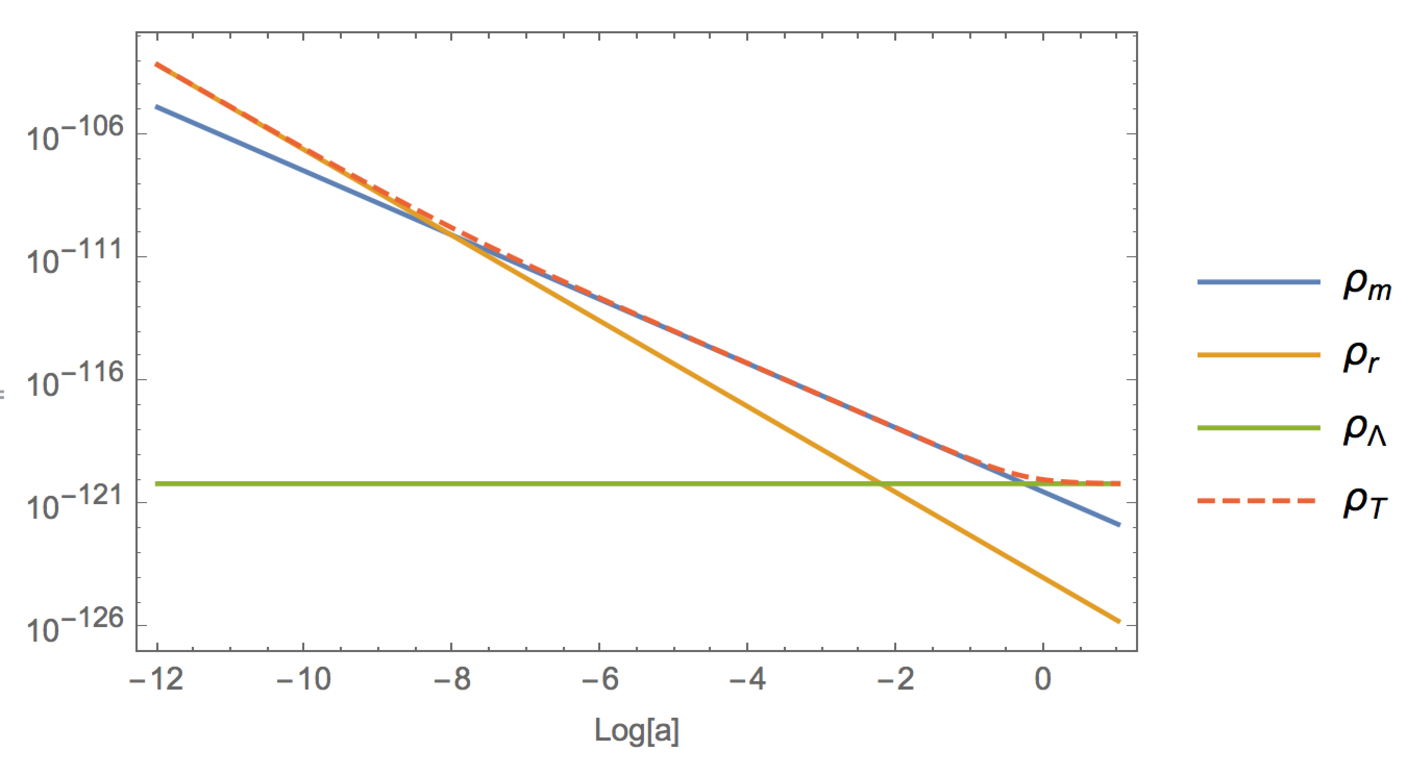
\includegraphics[width = 0.7\textwidth]{Sections/Figures/EnergyDensityEvol.pdf}
    \caption{Energy density evolution for radiation $\rho_r$, non-relativistic matter $\rho_m$, (constant) dark energy $\rho_\Lambda$ and the total energy density, $\rho_T$ as a function of the scale factor in Planck units with $a_0=1$ today.}
    \label{fig:RhoEvol}
\end{figure}


\subsection{Major Events}
\label{subsecME}

The Hot Big Bang model for cosmology assumes that the universe was initially a hot soup of elementary particles at a very high temperature. In broad terms, the subsequent  evolution describes the cooling of this hot soup as the universe expands.  Indeed, conservation of entropy (for relativistic particles with a constant number of species) implies that temperature falls as 
\be
T(t)=T_0 \left(\frac{a_0}{a(t)}\right) \,,
\ee
and can be used as an alternative to time to parameterise the history of the universe.
There are two main consequences of such an expansion and cooling:
\begin{enumerate}
\item Reaction rates in dilute systems are generically proportional to the number of participants per unit volume, because the reactants must be able to find one another before they are able to react. Since  particle densities fall as the universal volume grows, reaction rates also fall. Thus interactions between particles freeze out when the interaction rate drops below the expansion rate. This implies that one of the main trends of cosmology is that, as the universe ages, thermal and chemical reactions fall out of equilibrium.

\item A consequence of the previous point is the appearance of bound states of particles as the universe ages. Although the reactions forming bound states can always occur, at the earliest epochs temperatures are high enough to ensure that collisions very efficiently destroy these bound states, leaving very few to survive in equilibrium conditions. As the temperature drops, the inter-particle collisions become less violent and eventually the reactions of formation can dominate to leave a population of primordial relic bound states. Moreover, in an expanding universe, broken symmetries in the laws of physics may be restored at high energies. At very early epochs, phase transitions are also expected to play an important role in the cosmic evolution, but as yet there is no direct evidence that such transitions took place.
\end{enumerate}

\begin{figure}[ht]
    \centering
    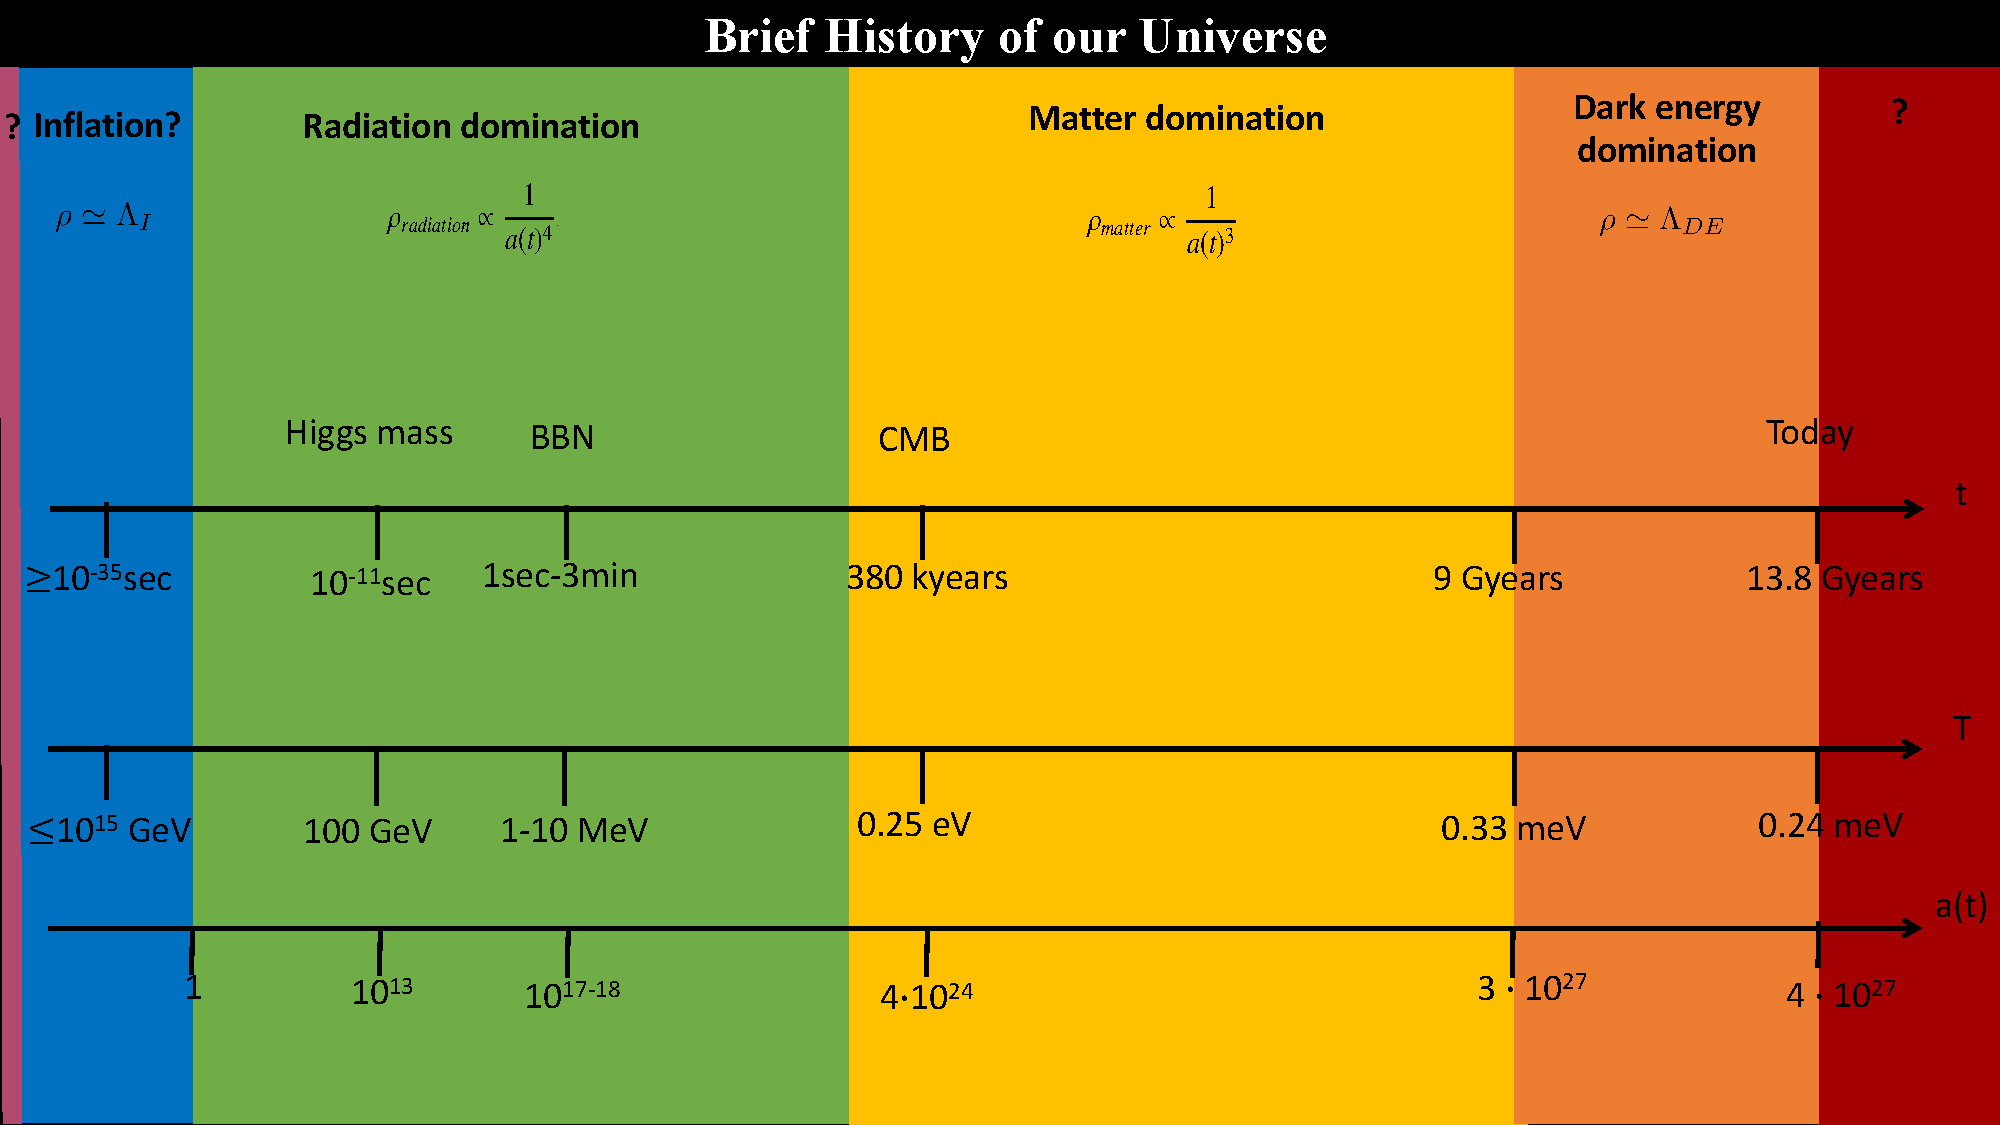
\includegraphics[width = 0.9\textwidth]{Sections/Figures/FigureHistory.pdf}
    \caption{A schematic representation of the different epochs and their temperatures within the history of the universe in
    the standard $\Lambda$CDM cosmological model.}
    \label{fig:History}
\end{figure}

The  main events constituting the history of our universe can be summarised as follows  (see Tab. \ref{tab:universe_evol} and Fig.~\ref{fig:History}).
\begin{itemize}
\item At  $t\sim 10^{-43}$ s ($10^{19}$ GeV), we are near the Planck scale, where we expect  quantum gravity effects, such as those of string theory,
to dominate and general relativity not to be valid.  One of the fundamental issues of spacetime structure at the Planckian scale is  the question of cosmic singularities.  It is expected that these problems will be  addressed in the, as yet not definitively known, non-perturbative quantum gravity theory.

\item The period from  $t\sim 10^{-43}-10^{-14}$ s corresponds to temperatures  of around $T \sim10^{19}$ GeV - $10^4$ GeV, which are not foreseeably accessible by accelerators. In this sense, the universe can be used to test fundamental physics relevant at this scales, such as supersymmetry,  grand unification, string theory, extra dimensions, and other theories. Perhaps the most interesting phenomenon in the above energy range is the accelerated expansion of the early universe, inflation, which, as will be discussed below, likely occurred  somewhere near grand unification scales.

\item The epoch from  $t\sim 10^{-14}-10^{-10}$ s, corresponding to temperatures of $T\sim 10^4$ GeV - $100$ GeV, may be accessible by accelerators.
In particular, the standard model of the electroweak and strong interactions  is applicable here.

\item At  $t\sim 10^{-5}$ s, the corresponding temperature $T\sim200$ MeV, the QCD scale, where the  quark-gluon transition takes place.

\item Between  $t\sim0.2$ s and $200-300$ s (where $T\sim 1-2$ MeV at the start and $T\sim0.05$ MeV at the end), we have temperatures at the nuclear physics scale. Two important events happen during this period. First, the primordial neutrinos decouple from the other particles and subsequently propagate without further scatterings. Second, the process of {\em primordial nucleosynthesis}  takes place.  The initial conditions for this are set by the `freeze out' of the ratio of neutrons to protons, when the interactions that keep these particles in chemical equilibrium become inefficient; the number of the surviving neutrons subsequently determines the abundances of the primordial elements. As nuclear reactions become efficient, previously free protons and neutrons form helium and other light elements. The abundances of the light elements resulting from Big Bang Nucleosynthesis (BBN) are in very good agreement with observations, and this strongly supports our understanding of the universe's evolution back to the first second after the big bang.
 
\item $t\sim10^{11}$ s ($T\sim$ eV). This time corresponds to matter-radiation equality, which separates the radiation-dominated epoch from the matter-dominated epoch.

\item  At $t\sim 10^{12}-10^{13}$ s another two related important event happens. During so-called `recombination', nearly all free electrons and protons combine to form neutral hydrogen.  At this stage, the photons decouple and the universe becomes transparent to the background radiation. The Cosmic Microwave Background (CMB) temperature fluctuations, induced by the slightly inhomogeneous matter distribution at photon decoupling, form and survive to the present day, delivering direct information about the state of the universe at the last scattering surface.

\item Finally, at our present time $t\sim 10^{16}-10^{17}$ s,  galaxies and their clusters have formed from  small primordial inhomogeneities as a result of gravitational instability. An important question regarding this period is the nature of both dark matter and also the dark energy which is driving the present day accelerated expansion.
\end{itemize}

\begin{table}
[H]
\begin{center}
\centering
\begin{tabular}{| l |  m{8em}  | m{10em}| m{10em} | m{10em} | }
\hline
\cellcolor[gray]{0.9}  {\bf Temperature} &  \cellcolor[gray]{0.9} {\bf Time }&  \cellcolor[gray]{0.9} {\bf Particle Physics } &  \cellcolor[gray]{0.9} {\bf Cosmological Event}   \\
\hline \hline
$10^{19} {\rm GeV}$   & $10^{-43} {\rm s}$ & Quantum Gravity & Gravitons decouple?   \\
\hline
$10^{19} {\rm GeV}$ -  $10^2 {\rm GeV}$   &  $10^{-43} {\rm s}$ - $10^{-12} {\rm s}$ & Grand Unification?  Desert? String theory? Extra dimensions?  &  Inflation? Topological defects? Baryogenesis?\\
\hline
 $10^2$ GeV & $10^{-12}$ s   & Electroweak Breaking & Baryogenesis?    \\
\hline
 $0.3$ GeV & $10^{-5}$ s   & QCD scale & Quark-Hadron transition    \\
\hline
 $10-0.1$ MeV & $10^{-2}$ - $10^2$ s   & Nuclear Physics Scale & Nucleosynthesis, Neutrinos decouple     \\
\hline
$10$ eV & $10^{11}$ s   & Atomic Physics Scale & Atoms formed, CMB, Matter domination     \\
\hline
\end{tabular}
\end{center}
\caption {Brief history of our universe. Temperature units can be transformed to Kelvin using the conversion factor $1\,{\rm GeV}\, =1.16 \times 10^{13}$ K.}
\label{tab:universe_evol}
\end{table}

The standard cosmological model just discussed describes a simple and consistent picture of the relatively recent universe,  which is able to account for the many available observations of the overall structure and evolution of the universe. This picture bears up to scrutiny very well, at least for all times after the epoch of BBN. This success however, comes with some drawbacks, which  can be summarised as follows:

\begin{itemize}

\item  {\em The horizon problem}.  The CMB radiation, first discovered in 1964, is known with excellent precision and  is landmark evidence of the Big Bang origin of the universe. 
One of its most striking features is that its variations in intensity across the sky are tiny, less than 0.01\% on average.
It follows from this that the universe was extremely homogeneous at the time of recombination. Assuming the standard expansion of the universe,
we receive the same physical information from causally disconnected regions of space. It is (apparently) a puzzle why the radiation is so uniform.

\item {\em The flatness problem.}  The most recent results from the CMB are consistent with a flat universe. Namely, the  position and height of the first acoustic peak on the spectrum of the CMB provides evidence for $\Omega=1$ (see \eqref{eq:OmegaGeo}) \cite{Planck:2018vyg}.
 The flatness problem refers to the fact that for $\Omega$ to be so close to one at present, it had to be essentially one in the early universe to extraordinarily high precision, which also constitutes an apparent puzzle.

\item {\em Dark matter \& Dark Energy}. The standard cosmological model, supported by the most recent data \cite{Planck:2018vyg},  postulates the existence of two new forms of matter, namely dark matter and dark energy,  for which there is  no direct evidence from particle physics or from Earth-based experiments.

\begin{itemize}

\item Dark matter: Besides CMB evidence for dark matter, the survey and study of the behaviour of matter, such as rotation curves of galaxies, at many different scales, has given evidence that there should be a new kind of matter, not present in the standard model of particle physics. This plays  an important role in the explanation of the large scale structure formation. We still do not know what dark matter is: is it a particle, or some sort of  massive compact object present in the universe?

\item Dark energy: Recent results form the study of high redshifted supernovae, combined with CMB results provide strong evidence for the fact that the universe is  accelerating today ($\ln a\sim -0.34$, see Fig. \ref{fig:RhoEvol}). This indicates that there should be a form of `dark energy' satisfying eq.~\eqref{eq:rho3p} $(\rho+3 p)<0$ and thus causing the universe to accelerate today. Either an effective cosmological constant or a time varying scalar field,
called {\em quintessence},  are the main proposals for this dark energy.
\end{itemize}
\end{itemize}

All of these problems are strong guides as to the nature of necessary extensions beyond the Hot Big Bang, and in general to the need for physics beyond that contained in the Standard Model of particle physics.

\subsection{Cosmological Inflation}
\label{sec:infla}

Cosmic Inflation was initially motivated as a way to address the flatness and horizon problems above.  Quite compellingly, it was later found that it also provides a simple explanation for the origin of the primordial density fluctuations which seeded the observed temperature fluctuations of the CMB and the formation of galaxies through gravitational collapse.

The main idea behind inflation is that the  universe underwent a period of accelerated expansion at some point in its very distant past. If the inflationary period is long enough, it rapidly flattens the universe, solving the flatness problem. It also explains why some regions could be in causal contact with each other, solving the horizon problem. Requiring that inflation solves both the flatness and horizon problems, one can estimate that inflation should last for $N\gtrsim 60$ e-foldings.

\bigskip

An accelerated expansion implies that
\be
\ddot a >0\,.
\ee
Using \eqref{eq:Hdef} we can express this condition as
\be
\label{eq:ddota}
\frac{\ddot a}{a} = H^2\lb1-\epsilon \rb >0 \,,
\ee
where we introduce the {\em slow-roll} parameter $\epsilon$, defined as
\be
\label{eq:epsdef}
\setlength\fboxsep{0.25cm}
\setlength\fboxrule{0.4pt}
\boxed{
\epsilon\equiv -\frac{\dot H}{H^2}\,,
}
\ee
and thus the condition for an accelerated universe is encoded in the requirement that
\be
\label{eq:epscond}
\epsilon<1 \,.
\ee
Using  \eqref{eq:Fried4DH} and \eqref{eq:EMconsFLRW} in \eqref{eq:epsdef}, we can write $\epsilon$ as
\be
\setlength\fboxsep{0.25cm}
\setlength\fboxrule{0.4pt}
\boxed{
\epsilon \equiv \frac{3}{2}(1+\omega)\,,
}
\ee
and thus $\epsilon <1$ implies the condition  \eqref{eq:omega_acc} for an accelerated expansion, as seen previously.

This  is equivalent to the statement that  the {\em comoving Hubble radius} $(aH)^{-1}$ shrinks in accelerated expansion,
rather than the growing behaviour of radiation and matter dominated phases. That is,
\be
\frac{d}{d t}(aH)^{-1} = -\frac{1}{a} \lb 1-\epsilon \rb <0.
\ee
In a universe dominated by a fluid with equation of state $p=\omega \rho$, the comoving Hubble radius behaves as
\be
\frac{1}{aH} \sim t^{\frac{\epsilon-1}{\epsilon}}\,,
\ee
and thus again we see that $\epsilon<1$ implies that the comoving Hubble radius decreases, while for $\epsilon>1$, it increases.
For example, during matter domination $\omega=0$ and $\epsilon = 3/2$, while during radiation domination $\omega=1/3$ and $\epsilon=2$.
Note that as soon as the condition $\epsilon<1$ fails, inflation ends and thus we can define the end of inflation as $\epsilon\sim 1$.

\begin{figure}[ht]
    \centering
    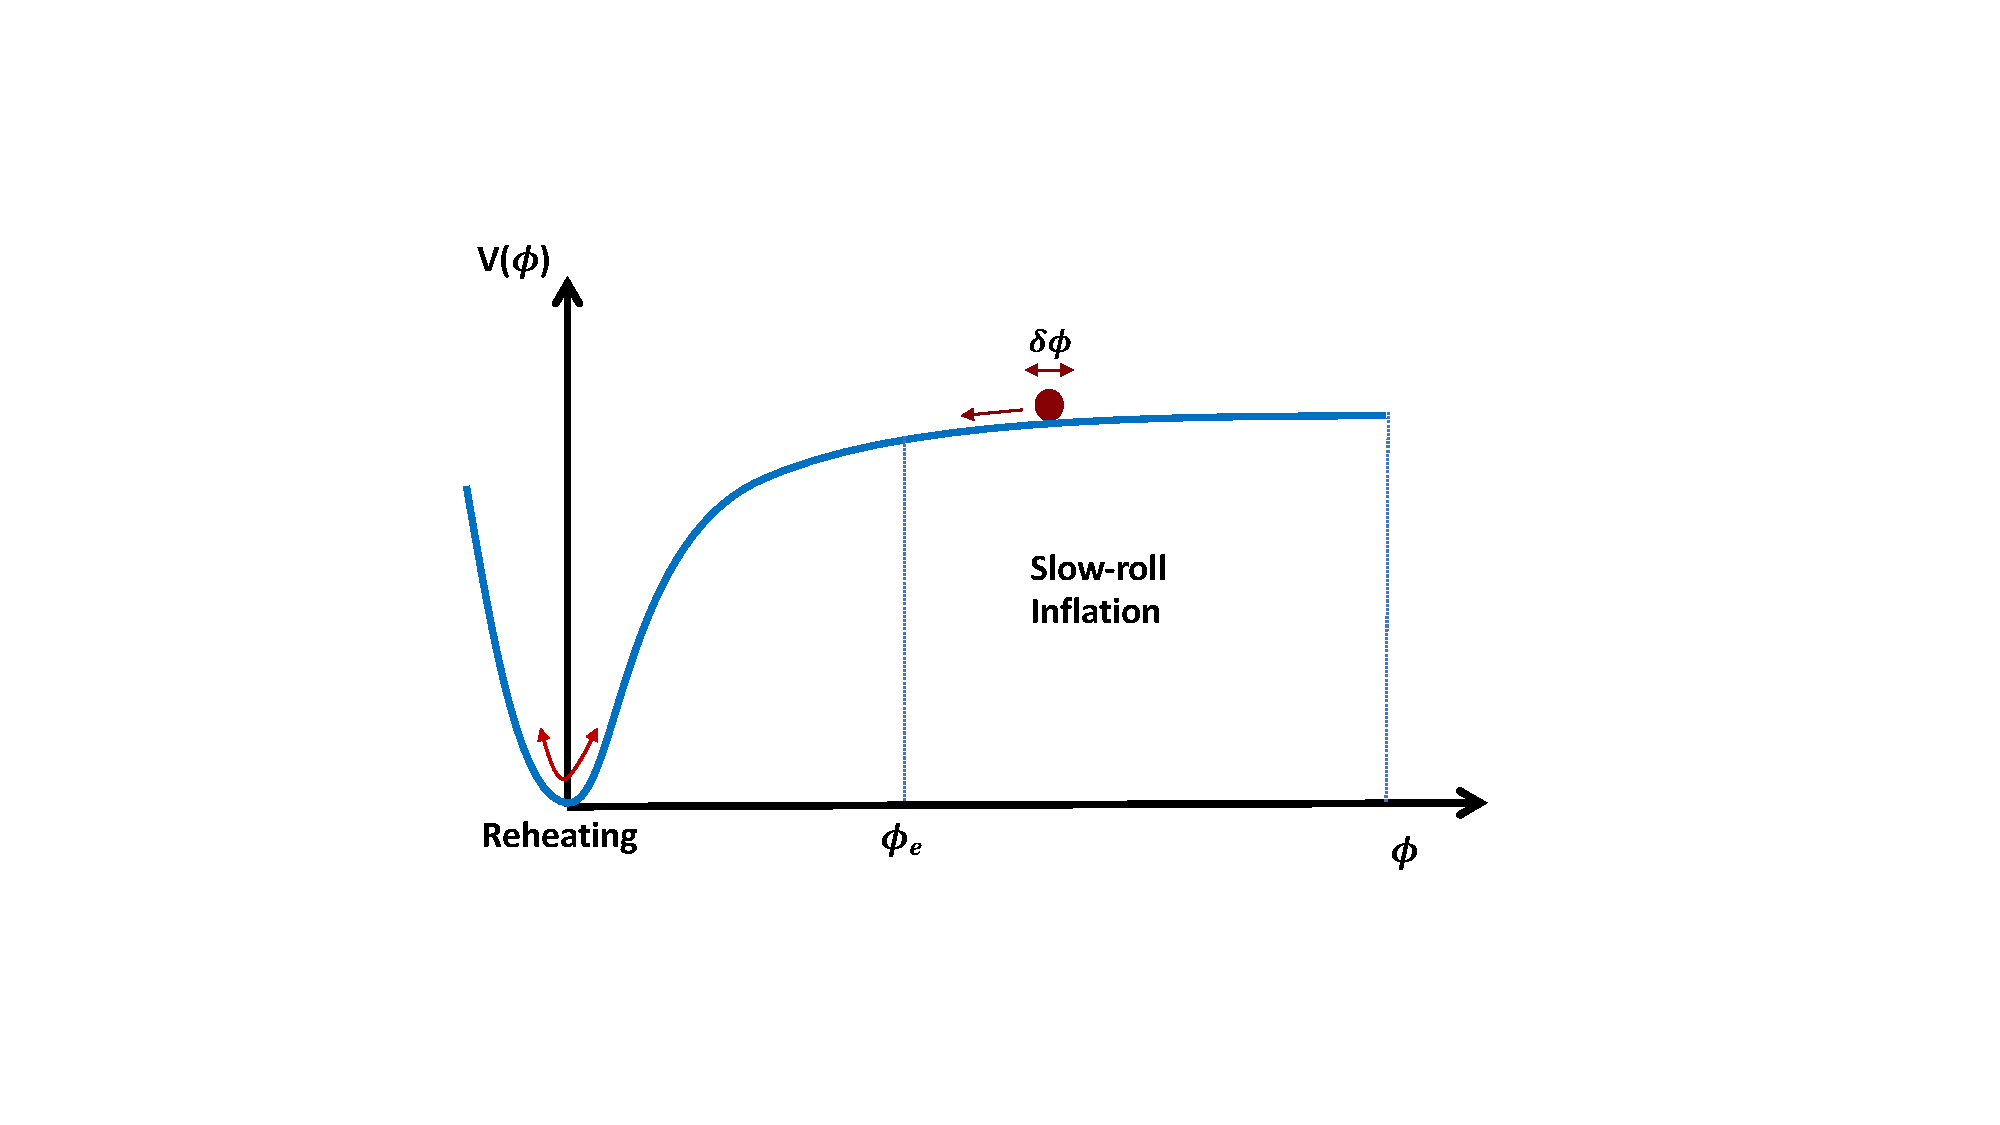
\includegraphics[width = 0.7\textwidth]{Sections/Figures/FigureInflation.pdf}
    \caption{An illustration of the standard picture of slow-roll inflation ending in fast roll of the inflation to a minimum and subsequent reheating of the universe.}
    \label{fig:Inflation}
\end{figure}

In the de Sitter limit, $\epsilon\to0$, the space grows exponentially as in \eqref{eq:dSa}. More generally, an inflationary expansion requires a somewhat unconventional matter content. Indeed, from \eqref{eq:Fried4Da} we see that, for a universe supported by a perfect fluid, the energy density and pressure should satisfy
\be
\rho+3p <0 \,,
\ee
that is, the overall pressure of the universe should be negative $p <-\rho/3$, which corresponds 
to a violation of the {\em strong energy condition} (SEC)\footnote{The SEC for a perfect fluid states that $\rho+p\geq 0$ \cite{Hawking:1973uf}.}.This occurs in neither radiation nor matter dominated phases (for which $p=\rho/3, p=0$ respectively).
However, one simple energy source that can drive inflation is the  positive potential energy  of a single (canonically normalised) scalar field with negligible kinetic energy (see Fig.~{fig:Inflation} for an illustrative example). As we will encounter later, other alternatives are also possible.

\subsubsection{Slow-roll conditions}

Let us consider a single (canonically normalised) scalar field,  {\em the  inflaton}, with potential energy $V$, coupled to gravity.  Its 
action reads
\be
\label{eq:scalarS}
S= \int{d^4x \sqrt{- g} \left[\frac{1}{8\pi\,G_4} \,\frac{R_4}{2}  - \frac{1}{2} \partial_\mu\varphi\, \partial^\mu\varphi - V(\varphi)\right]} \,.
\ee
Although the inflaton can in principle depend on both time and space, inflation rapidly smooths out spatial variations, and thus for the background evolution, it suffices to study\footnote{The spatial dependence will be relevant later for the quantum fluctuations of the inflaton.} $\varphi=\varphi(t)$.
In a spatially flat FLRW spacetime \eqref{eq:FLRW} the variation of the action \eqref{eq:scalarS} with respect to $\varphi$ gives
\be
\label{eq:phieq}
 \ddot \varphi + 3H\dot\varphi+  V_{,\varphi} =0  \,.
\ee
The energy momentum tensor of the field derived from \eqref{eq:scalarS} gives
\be
T_{\mu\nu} = \partial_\mu\varphi\partial_\nu\varphi -g_{\mu\nu}\lb \frac12 (\partial\varphi)^2 +V(\varphi)\rb\,.
\ee
In the flat FLRW background, the energy density and pressure of the scalar are found to be
\begin{subequations}
 \begin{align}
 \label{eq:rhoscalar}
\rho_\varphi& = \frac{1}{2} \dot \varphi^2 +V(\varphi)\,, \\
p_\varphi &= \frac{1}{2} \dot \varphi^2 -V(\varphi)\,.\label{eq:Pscalar}
\end{align}
\end{subequations}
With this, eqs. \eqref{eq:Fried4DH} and \eqref{eq:Fried4Da} yield
\bea
&&H^2 = \frac{8\pi\,G_4}{3} \left(\frac{\dot \varphi^2}{2}  + V(\varphi)\right) \,, \label{eq:Hscalar} \\
&& \frac{\ddot a}{a} = -\frac{8\pi\,G_4}{3} \lp \dot\varphi^2 -V(\varphi) \rp  \,.
\label{eq:Rayscalar}
\eea
We now introduce the slow-roll conditions. A nearly exponential expansion can be ensured by the requirement that the fractional change of the Hubble
parameter per e-fold $N$ is small, that is $\epsilon \ll1 $ (see eq.~\eqref{eq:epsdef}). In terms of the inflaton,
$\varphi$, this can be written as (from now on we use $\Mp$ rather than $G_4$)
\be
\label{eq:epsfi}
\epsilon = \frac{\dot\varphi^2}{2 \Mp^2 H^2} \ll 1\,.
\ee
Requiring that inflation lasts for a sufficiently long time that the horizon problem is solved is equivalent to requiring that $\epsilon$ remain small for a sufficient number of Hubble times, which is measured by the {\em second slow-roll} parameter, $\eta$, defined as
\be
\label{eq:etafi}
\setlength\fboxsep{0.25cm}
\setlength\fboxrule{0.4pt}
\boxed{
\eta\equiv \frac{\dot \epsilon}{H\epsilon} = \frac{\ddot H}{H\dot H} + 2\epsilon = 2\frac{\ddot \varphi}{H\varphi} + 2\epsilon\,.
}
\ee
This then implies that $\delta_\varphi\ll1$, where we defined 
\be
\label{eq:deltafi}
\setlength\fboxsep{0.25cm}
\setlength\fboxrule{0.4pt}
\boxed{
\delta_\varphi \equiv \frac{\ddot \varphi}{H\dot\varphi}  \,.
}
\ee
 Using the Friedman equation \eqref{eq:Hscalar}, we  see that the first slow-roll condition \eqref{eq:epsfi}, implies
that $\dot\varphi^2 \ll V$ and therefore we can write \eqref{eq:Hscalar} as
\be
\label{eq:Hslowr}
H^2 \simeq \frac{V(\varphi)}{3 \Mp^2} \,.
\ee
Moreover, using \eqref{eq:deltafi}, we can write \eqref{eq:phieq} as
\be
\label{eq:fislowr}
3H\dot \varphi + V_{,\varphi} \simeq0\,.
 \ee

In the present case of a single scalar field, we can write the slow-roll conditions \eqref{eq:epsfi} and \eqref{eq:deltafi} (equivalently \eqref{eq:etafi}) solely in terms of the scalar potential and its derivatives as follows.  From the condition \eqref{eq:epsfi}, using \eqref{eq:fislowr} and \eqref{eq:Hslowr}, we arrive at
\be\label{eq:epsV}
\setlength\fboxsep{0.25cm}
\setlength\fboxrule{0.4pt}
\boxed{
  \epsilon_V\equiv \frac{\Mp^2}{2} \lp\frac{V_{,\varphi}}{V}\rp^2 \simeq \epsilon \,,
  }
\ee
which is the first {\em potential slow-roll parameter}.
Next, using the conditions \eqref{eq:fislowr} and  \eqref{eq:Hslowr} in \eqref{eq:deltafi}, we obtain
\be
\Mp^2 \frac{V_{,\varphi\varphi}}{V} + \epsilon \ll 1\,,
\ee
and so therefore introduce the second potential slow-roll parameter,  $\eta_V$,
\be\label{eq:etaV}
\setlength\fboxsep{0.25cm}
\setlength\fboxrule{0.4pt}
\boxed{
\eta_V \equiv \Mp^2 \,\Bigg|\frac{V_{,\varphi\varphi}}{V} \Bigg|\,.
}
\ee
Thus, {\em in single field inflation}, the slow-roll parameters can be written in terms of the scalar potential and its derivatives, which need to be  small during  inflation:
\be
\epsilon_V \ll1 \,,\qquad \eta_V\ll1 \,.
\ee
Note that in this case, the smallness of the $\eta_V$-parameter (which in the present single field case is equivalent to $\eta$ and $\delta_\varphi$),  implies that the mass of the inflation, $|m_{\rm inf}^2| \sim |V_{,\varphi\varphi}| \ll H^2$ 
(as we will see, this conclusion no longer holds when more scalar fields are present \cite{Chakraborty:2019dfh,Aragam:2021scu}). The required smallness of the slow-roll parameters, and in particular the mass of the inflaton, is vulnerable to quantum corrections, as we will discuss in detail when we consider UV complete models in Sec. \ref{sec:infla}.

\subsubsection{Primordial fluctuations}\label{sec:PrimF}

As we have seen, the early universe is supposed to have been rendered very nearly uniform by a primordial inflationary epoch. According to our current understanding, structures in the universe originated from tiny `seed' perturbations, which grew to form  all the structures we observe today.
Observations of the CMB support this view, indicating that at the time of decoupling the universe was very nearly homogeneous with small inhomogeneities at the $10^{-5}$ level.
The best candidate for the origin of these perturbations is quantum fluctuations produced during  inflation  in the early universe.
 These perturbations extend from extremely short scales to cosmological scales by the stretching of space during inflation.
%
\begin{center}
\begin{figure}[H]
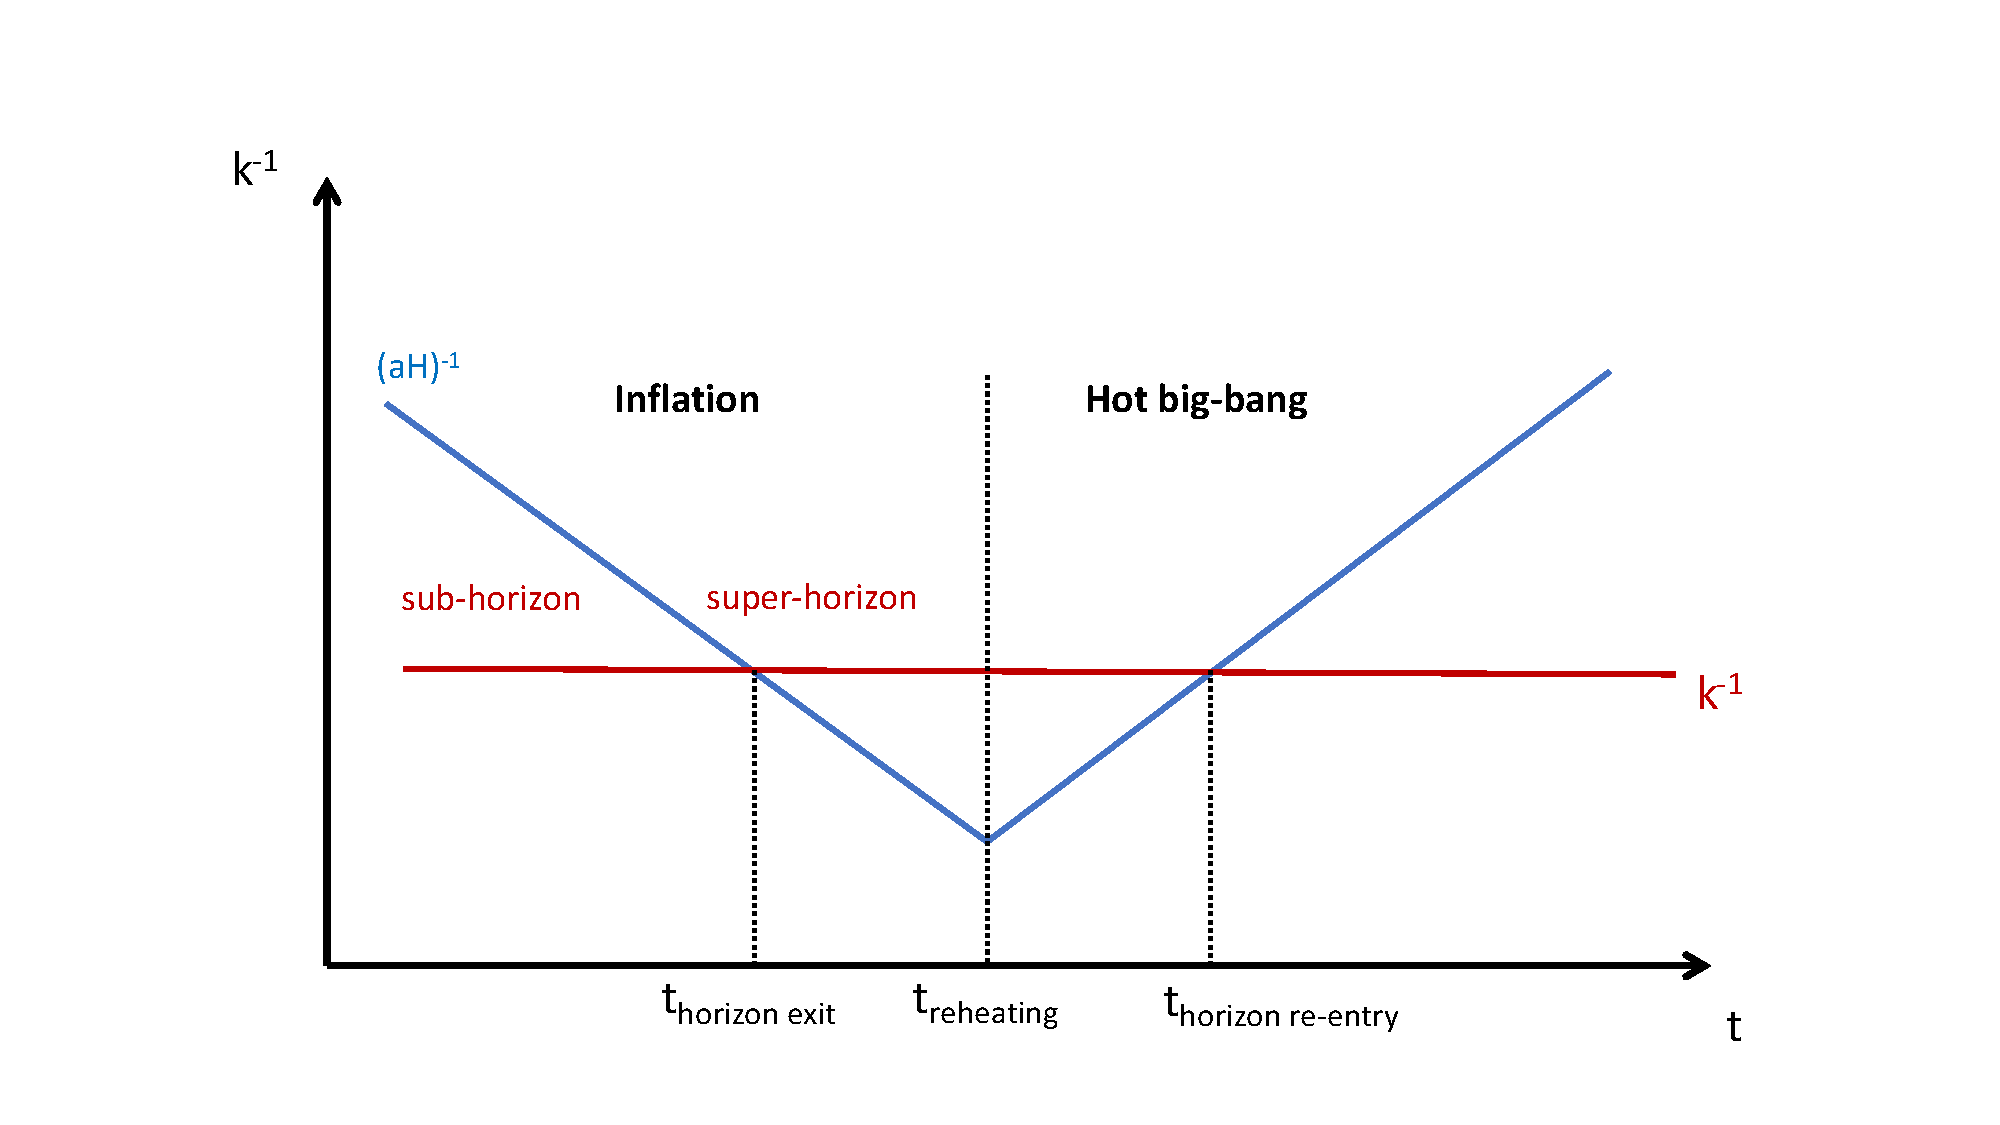
\includegraphics[width=14cm]{Sections/Figures/DensityPerturbations.pdf}
\caption{Horizon exit and re-entry of a density perturbation with wave number $k$.}
\label{Fig:perturbations}
\end{figure}
\end{center}
%
The shrinking of the comoving Hubble radius (Hubble horizon) during inflation implies that fluctuations leave the horizon at some point (see Fig.~\ref{Fig:perturbations}).  Once inflation  ends,  the Hubble radius increases and  the fluctuations eventually reenter it during the radiation -- or matter -- dominated epochs. Fluctuations that exit the horizon around 60 e-foldings or so before the end of inflation, reenter with physical wavelengths in the range accessible to cosmological observations, with the CMB probing around 7-10 e-folds (note that the number 60 here depends on the post-inflationary evolution which, as discussed in Sec. \ref{reheating}, can be quite different in stringy scenarios compared to the vanilla picture of immediate reheating; see \cite{Bhattacharya:2017ysa, Bhattacharya:2017pws} for discussions in a stringy context). The spectra generated for density perturbations and gravitational waves during inflation provide a distinctive signature and can be measured by analysing the microwave background radiation anisotropies.


During inflation,  the inflaton field dominates the energy density of the universe, and thus any perturbation on it  implies  a perturbation of the  energy-momentum tensor
\be
\delta\varphi \quad  \Longleftrightarrow  \quad \delta T^{\mu\nu}\,.
\ee
A perturbation in the energy-momentum tensor then implies, via Einstein's equations of motion, a perturbation of the metric
\be
\delta G_{\mu\nu} =  \lp \delta(R_{\mu\nu}) -\frac12\delta(g_{\mu\nu}\,R)\rp = 8\pi G \delta T^{\mu\nu} \, ,
\ee
and so we have
\be
\delta\varphi \quad  \Longleftrightarrow \quad \delta g_{\mu\nu}\,.
\ee
The metric perturbations can be decomposed according to their spin into {\em scalar}, {\em vector} and {\em tensor} perturbations with respect to rotations of spatial coordinates on hypersurfaces of constant time. At  linear order, the scalar, vector and tensor perturbations evolve independently (decouple) and it is thus possible to analyse them separately. Vector perturbations do not get excited during inflation because there are no rotational velocity fields. In what follows, we summarise the analysis of scalar and tensor perturbations in inflation. For more details see e.g.~\cite{Mukhanov:1990me,Riotto:2002yw}.

\subsubsection*{Gauge choice}

An important  subtlety in the study of cosmological perturbations is that  the split into background and perturbations  is not unique, but depends on the choice of coordinates or the gauge choice.  It is important to note that there is no preferred gauge.  
To eliminate this ambiguity, one has two choices:
either identify  {\em gauge invariant} quantities or choose a given gauge and perform the calculations in that gauge.
Both options have advantages and drawbacks. By selecting a certain gauge, the calculations might be made technically simpler, but there is a risk that doing so introduces gauge artifacts or unphysical perturbations. On the other hand, a gauge-invariant computation may be technically more involved, but has the advantage of dealing only with physical quantities.

\subsubsection*{Gauge-invariant variables}

As we discussed above, it is helpful to provide gauge-invariant combinations of metric and matter perturbations in order to avoid the problem of spurious gauge modes. There are three gauge invariant quantities that are usually  defined in calculations of inflation: \\

\begin{tcolorbox}[title={\bf Gauge invariant variables}]

\begin{enumerate}[i.]
\item The {\em comoving curvature perturbation}. This is given by
\be\label{eq:curvatureR}
{\cal R} =\Psi + H\, \frac{\delta\varphi}{\dot\varphi} \,,
\ee
where $\Psi$ is the spatial {\em curvature perturbation}. In geometrical terms, $\cal R$  measures the spatial curvature of comoving hypersurfaces.

\item The {\em curvature perturbation on slices of uniform energy density}. This is given by
\be
\zeta = \Psi -\frac{\delta\rho}{3(\rho+p)}\,.
\ee
Geometrically, $\zeta$ measures the spatial curvature of constant-density hypersurfaces.
 For a scalar field, $(\rho+p) =\dot\varphi^2$. Moreover, during inflation   $\delta\rho \simeq-3H\,\dot\varphi\,\delta \varphi$.  Thus
 $\zeta$ and $\cal R$ are  equal during slow-roll inflation. As we will see they are also equal on {\em super-horizon scales} and therefore the correlation functions of $\zeta$ and $\cal R$ are  the same at horizon crossing. Moreover,  both  are conserved on super-horizon scales during slow-roll inflation.

\item Scalar field perturbations in  {\em spatially flat gauge}. The {\em spatially flat gauge} is defined as the slicing where there is no curvature $\Psi=0$. It gives a  gauge-invariant measure of inflaton perturbations and is given by
\be
Q = \delta\varphi +\frac{\dot\varphi}{H}\,\Psi \,. 
\ee


\end{enumerate}

\end{tcolorbox}

\bigskip
One can compute the curvature perturbation generated during inflation on super-Hubble scales,  $\zeta$ or ${\cal R}$, either using a particular gauge and computing the gauge-invariant curvature in that gauge, or by doing a fully gauge-invariant calculation. The results are equivalent.

The gauge-invariant curvature perturbation $\cal R$ defined above   is conserved outside of the horizon. Thus, we can compute it   at {\em horizon exit} and remain ignorant about the sub-horizon physics during and after {\em reheating} until horizon re-entry of a given $\cal R$-mode, $k$.

The equation of motion for the curvature perturbation $\cal R$, takes a simple harmonic oscillator form  and thus it can be quantised by promoting the classical field $\cal R$ to a quantum operator and then quantising it. One can then compute the power spectrum of curvature fluctuations at horizon crossing.

We summarise the results and refer the reader to the bibliography for the details on the computations \cite{Riotto:2002yw}. 


\subsubsection*{Scalar perturbations}

The mode equation of motion for the Fourier components of $\cal R$ is given by
\be
\label{eq:R}
\setlength\fboxsep{0.25cm}
\setlength\fboxrule{0.4pt}
\boxed{
\cR''_k + 2\frac{z'}{z}\,\cR_k'+k^2\,\cR_k=0\,,
}
\ee
where here a prime denotes derivative with respect to  conformal time
$\eta$, $d\eta = dt/a(t)$; $k$ is the wavenumber and $z\equiv a\,\dot\varphi/H$, sometimes referred to as the {\em pump field}, which satisfies
\be
\label{eq:pumpf}
\setlength\fboxsep{0.25cm}
\setlength\fboxrule{0.4pt}
\boxed{
\frac{z'}{z} = aH\lp 1+\epsilon-\delta\rp\,,
}
\ee
where we have defined\footnote{Note from \eqref{eq:etafi} that $\eta=-2\delta+2\epsilon$. Note also the difference between $\delta$, determined by the full energy density and $\delta_\varphi$, which is associated only to the dynamics of a scalar fluid(s) component.}
\be
\setlength\fboxsep{0.25cm}
\setlength\fboxrule{0.4pt}
\boxed{
\delta\equiv -\frac{\ddot H}{2H\dot H}\,.
}
\ee
Let us note that fluctuations are created on all length scales, $\lambda$.
Relating the length scale  with its wavenumber $k$, as $\lambda = 2\pi a/k$
this means that the fluctuations are created with a spectrum of wavenumbers, $k$. Fluctuations that are cosmologically relevant start their lives inside the horizon (i.e.~Hubble radius), that is $k/aH\gg 1$.
However, while the comoving wavenumber is constant the comoving Hubble radius shrinks during  inflation. Scales for 
which  $k/aH\ll 1$ are outside the Hubble radius; eventually, all fluctuations exit the horizon. Thus we refer to the scales as follows (see Fig.~\ref{Fig:perturbations}):

\begin{subequations}\label{eq:scales}
\begin{empheq}[box=\widefbox]{align}
 &\frac{k}{aH}\gg 1 \qquad \Rightarrow \qquad \text{sub-horizon scales} \nonumber\\
&\frac{k}{aH}\ll 1 \qquad \Rightarrow \qquad \text{super-horizon scales} \nonumber
\end{empheq}
\end{subequations}

\ni For scales well outside the horizon, the solutions to \eqref{eq:R} are given by
\be
\label{eq:Rsuperhor}
\cR_k(\eta) = \cC_1 + \cC_2 \int\frac{d\eta}{z^2}\,,
\ee
where $\cC_1$ and $\cC_2$ are integration constants. From \eqref{eq:pumpf} we have
\be\label{eq:zsol}
z(a) = z_0 \,{\rm exp}\lb \int{ (1+\epsilon-\delta) \,d\ln a}\rb\,,
\ee
and therefore we see that during slow-roll,  when $\epsilon, \delta\ll 1$, $z\sim a$. Since  in this case $a\sim -1/(H\eta)$ we see that the term proportional to $\cC_2$ in \eqref{eq:Rsuperhor} decays rapidly as $a^{-3}$  outside the horizon, and is thus called the {\em decaying mode}. The  curvature perturbation is conserved at super-horizon scales and controlled by the {\em constant mode} $\cC_1$.
We thus see that the constancy of ${\cal R}_k$ depends on $\epsilon$ and $\delta$ doing nothing dramatic even after horizon crossing.
However, a more dramatic situation can  arise from a failure of slow-roll. If at any time after horizon crossing the friction term in \eqref{eq:R} changes sign,  becoming a negative driving term, the decaying mode can become a growing mode with interesting cosmological implications \cite{Leach:2000yw,Leach:2001zf,Ozsoy:2018flq}. This change of sign can occur whenever $z$ reaches a local maximum, that is,  whenever $1+\epsilon-\delta=0$. Since $\epsilon$ is always positive, $\delta$ must be at least one for this to happen. This can occur during a transient period of fast-roll, ultra slow-roll  or non slow-roll period. We review below briefly this possibility.

The  amplitude of the scalar power spectrum at leading order in slow-roll can be obtained by matching the super-horizon solution with the Bunch-Davies vacuum at sub-horizon scales, to obtain\footnote{This is sometimes denoted as $\cP_\cR$ or $\Delta_s$.}:
\be
\setlength\fboxsep{0.25cm}
\setlength\fboxrule{0.4pt}
\boxed{
\cP_\cR = \frac{ H^4}{(2\pi)^2\,\dot\varphi^2}\,\Bigg|_{k=aH} = \frac{H^2}{8\pi^2\Mp^2 \,\epsilon }\,\Bigg|_{k=aH}\,,}
\ee
where all quantities are evaluated at {\em horizon crossing}, $k=aH$ and we have used \eqref{eq:epsfi} in the last equality. The power spectrum of the  cosmic microwave background scalar fluctuations is shown in Figure \ref{Fig:Spectrum}. 

\begin{figure}[t]
\begin{center}
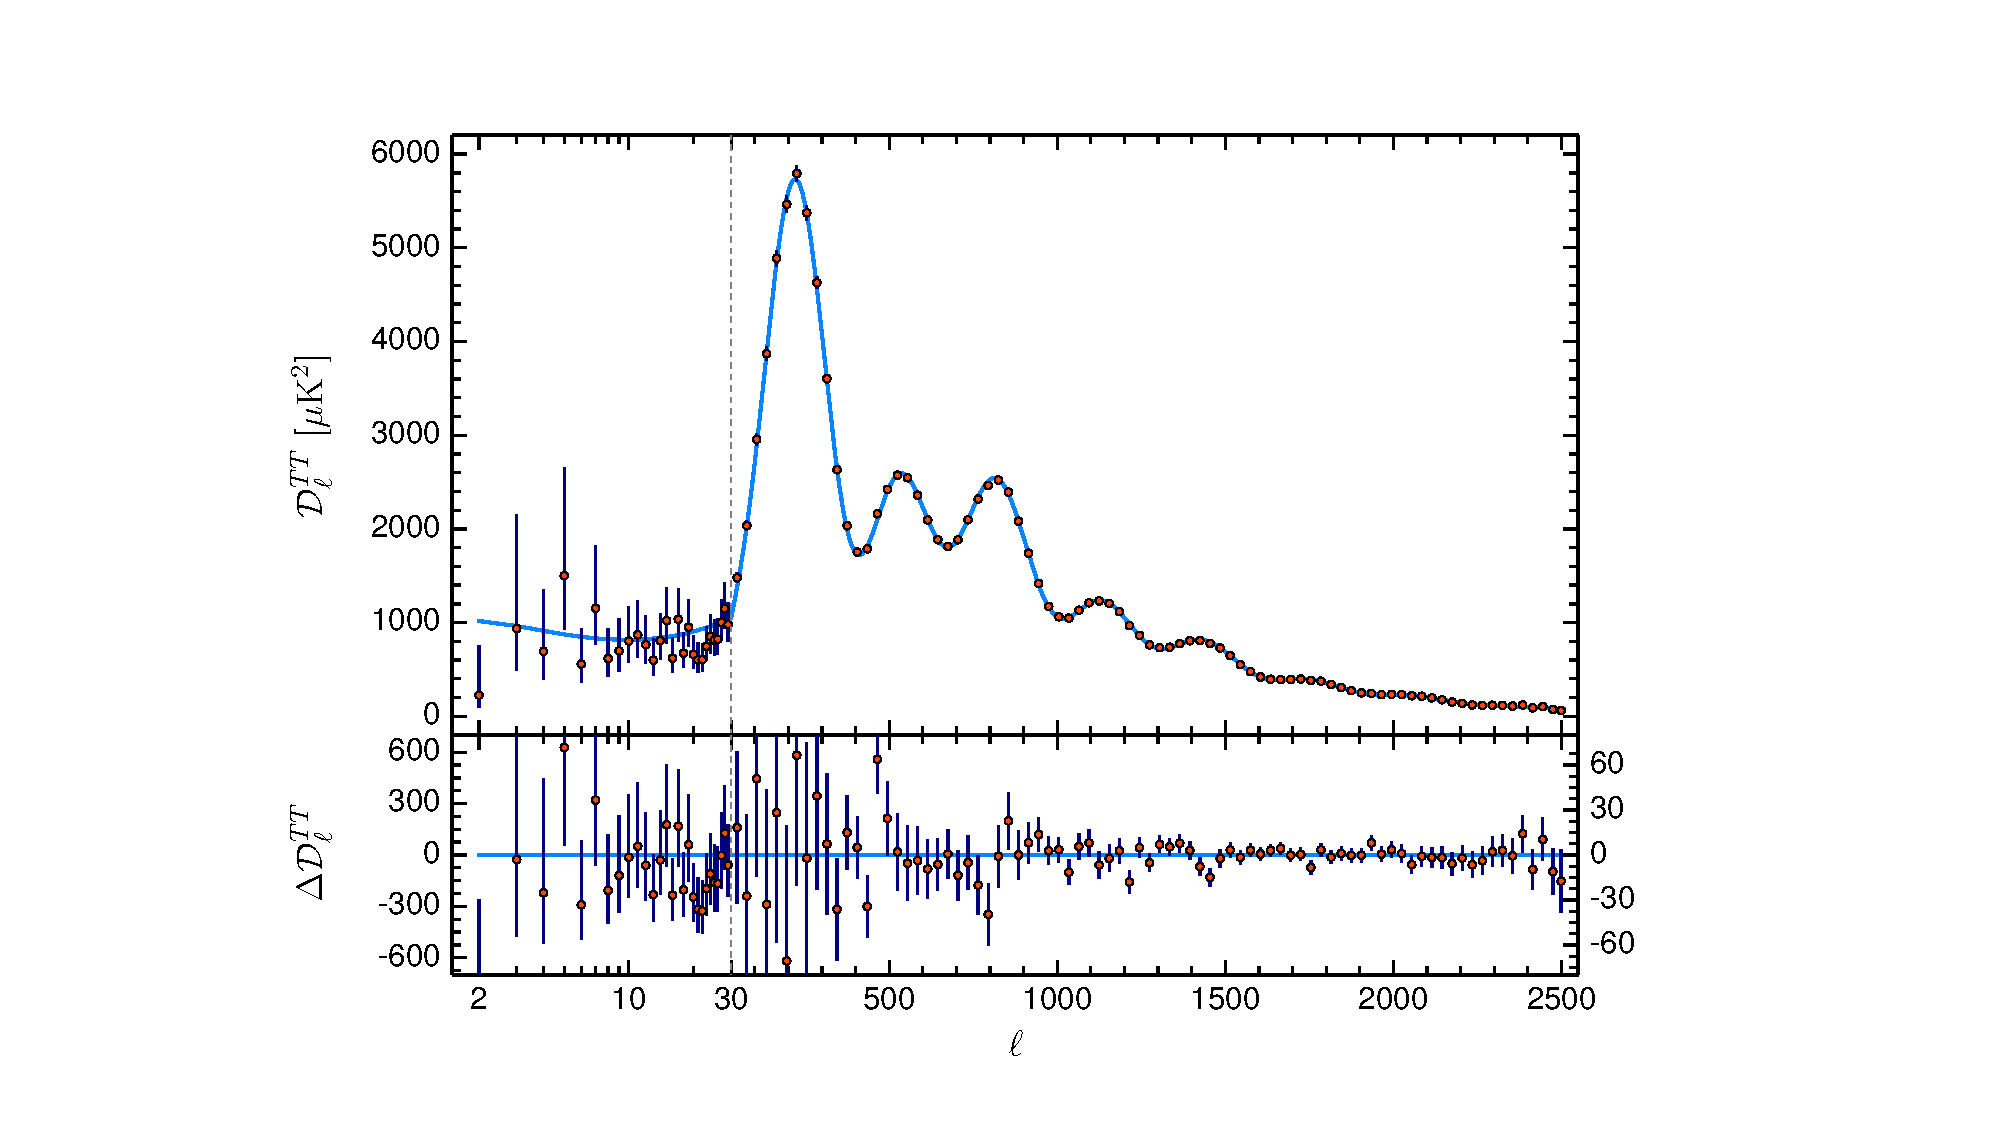
\includegraphics[width=145mm,height=105mm]{Sections/Figures/CMBSpectrum.pdf} 
\caption{The power spectrum of the scalar fluctuations of the cosmic microwave background including error bars for the $\Lambda$CDM model. This is one of most impressive examples of the precision level ($\simeq 10^{-5}$)  reached in cosmology so far, in which only a handful of parameters is enough to explain such a large number of data points (taken from \cite{Planck:2018vyg}). } \label{Fig:Spectrum} 
\end{center}
\end{figure}


\subsubsection*{Primordial tensor perturbations}

Quantum fluctuations in the gravitational field are generated in a similar fashion as the scalar perturbations discussed so far.
In general, the linear tensor perturbations may be written as
\be
ds^2 = a^2(\eta)\lb -d\eta^2 +(\delta_{ij}+h_{ij}) dx^idx^j\rb\,,
\ee
with $h_{ij}\ll1$. If the energy momentum tensor is diagonal, as is the case in the simplest inflationary model we have discussed so far,  the tensor modes do not have any source and their action is that of two (not yet canonically normalised) independent massless scalar fields\footnote{The tensor $h_{ij}$ has six degrees of freedom, but  tensor perturbations are traceless,  $h^i_i=0$, and transverse $\partial^ih_{ij}=0,  (i = 1,2,3)$. These are four constraints, that leave only  two physical degrees of freedom, or polarisations.}.

The corresponding canonically normalised field (dropping $ij$ indices),
\be
v_k \equiv  \frac{a}{2}\Mp \, h_k\,,
\ee
satisfies the equation of motion
\be
\label{eq:tensoreq}
v_k'' +\lp k^2 -\frac{a''}{a}\rp v_k =0\,,
\ee
which is the equation of motion of a massless scalar field  in a quasi-de Sitter epoch. It is interesting to note that, contrary to the scalar case, no  interesting effects arising from transient violations of slow-roll can occur for gravitational waves in standard GR.\footnote{However, in general scalar-tensor theories there can be non-trivial effects as discussed in \cite{Mylova:2018yap}.} This can be most easily seen as follows. Defining the field
\be
\psi_k = \frac{v_k}{a}\,,
\ee
Eq.~\eqref{eq:tensoreq} becomes
\be\label{eq:tensoreq2}
\psi_k'' + 2 aH \psi_k' + k^2 \psi_k =0\,.
\ee
As the `pump field' $a$ increases for all time, the constancy of the gravitational wave amplitude after horizon crossing is guaranteed until horizon re-entry \cite{Leach:2000yw}.

The  amplitude of the tensor power spectrum is  found to be
\be\label{eq:PT}
\setlength\fboxsep{0.25cm}
\setlength\fboxrule{0.4pt}
\boxed{
\cP_T = \frac{2}{\pi^2}\frac{H^2}{\Mp^2}\Bigg|_{k=aH}\,.}
\ee
Note that  this differs from the scalar power spectrum by depending only on the value of $H$ and not additionally on the slow-roll parameter $\epsilon$. Consequently, a comparison of both scalar and tensor modes  amplitudes provides a direct measure of the slow-roll parameter $\epsilon$. A more precise statement of this comparison is usually phrased in terms of the parameter $r$, defined as {\em tensor-to-scalar ratio} of the power spectra
\be\label{eq:rdef}
\setlength\fboxsep{0.25cm}
\setlength\fboxrule{0.4pt}
\boxed{
r\equiv \frac{\cP_T}{\cP_\cR} = 16 \,\epsilon\,.
}
\ee

\subsubsection{Scale dependence}

The scale dependence of the power spectra  is given by the spectral tilt indices and follows from the time-dependence of the Hubble parameter. The  scalar and tensor spectral indices are given, respectively, by
\be
\setlength\fboxsep{0.25cm}
\setlength\fboxrule{0.4pt}
\boxed{
n_s -1 \equiv \frac{d\ln \cP_\cR}{d\ln k} \,, \qquad \qquad n_t \equiv \frac{d\ln \cP_T }{d\ln k}\,.
}
\ee
Using that $d\ln k = H dt + d (\ln H)$ one finds, to first order in the Hubble slow-roll parameters
\begin{subequations}
\label{eq:nsnT}
\begin{empheq}[box=\widefbox]{align}
 n_s-1 &= -2\epsilon -\eta  \,,\\
n_T &= -2\epsilon\,,
\end{empheq}
\end{subequations}
where $\epsilon, \eta$ are defined in eqs.~\eqref{eq:epsdef} and \eqref{eq:etafi} respectively and these quantities are defined at horizon crossing.

We see that single-field slow-roll models satisfy a {\em consistency condition} between the tensor-to-scalar ratio $r$ and the tensor tilt $n_T$:
\be\label{eq:ccinfla}
\setlength\fboxsep{0.25cm}
\setlength\fboxrule{0.4pt}
\boxed{
r=-8\, n_T \,.
}
\ee
 If this relation were to be falsified by future observations of the CMB anisotropies, it would indicate that inflation was not driven by a single field.

 \subsubsection{Lyth bound}

Note that from eqs.~\eqref{eq:rdef} and \eqref{eq:epsfi}, we see that  the tensor-to-scalar ratio relates directly to the evolution of the inflaton as a function of the number of e-foldings $N=\int H dt$:
 \be
 r = \frac{8}{\Mp^2} \lp\frac{d\varphi}{dN}\rp^2\,.
 \ee
 Therefore,  the total field evolution, between the time when CMB fluctuations left the horizon at $N_{\rm hc}$ and the end of inflation at $N_{\rm end}$, is given by
 \be
 \frac{\Delta\varphi}{\Mp} = \int^{N_{\rm hc}}_{N_{\rm end}}{ dN \,\sqrt{\frac{r}{8}} } \,.
 \label{LythBound}
 \ee
 Making the conservative assumption that $r$ remains approximately constant during the inflationary period probed by the CMB, the inflaton must satisfy the so-called {\em Lyth bound} \footnote{Taking into account that the fact that $r$ does not
remain constant gives a much stronger bound \cite{Garcia-Bellido:2014wfa}.} \cite{Lyth:1996im,Boubekeur:2005zm}:
\be\label{eq:Lythbd}
\setlength\fboxsep{0.25cm}
\setlength\fboxrule{0.4pt}
\boxed{
\frac{\Delta\varphi}{\Mp} \gtrsim  \,2\times \lp\frac{r}{0.01} \rp^{1/2}\,.
}
\ee
This relation indicates that `large' values of the tensor-to-scalar ratio, $r \sim 0.01$, correlate with $\Delta\varphi \sim \Mp$, or {\em large-field inflation}. The vulnerability of large-field inflation to quantum corrections will be discussed in Sec. \ref{sec:infla}.

Using Eqs. \eqref{eq:PT} and \eqref{eq:rdef}, one can also immediately relate the Hubble parameter during inflation to the tensor-to-scalar ratio or slow-roll parameter $\epsilon$:
\be
H_{\rm inf} = \sqrt{8 \pi^2 \cP_\cR\,\epsilon}\, \Mp \,.
\ee
The observational constraints that we are about to summarise might then make a high GUT-scale, large-field inflation seem more likely in the context of a single inflaton field.

\subsubsection{Current inflationary constraints}

In this section we summarise the most recent CMB experimental results that have tested the physics of inflation \cite{Planck:2018jri} (see Fig.~\ref{Fig:SpectralIndex}). Let us start by providing the current best-fit value for the power spectrum amplitude, defined through
 \be
 \cP_\cR = A_s \lp\frac{k}{k_*}\rp^{n_s-1}\,,
 \ee
 where $k_*$ is a pivot scale taken at $k_*=0.05 {\rm Mpc}^{-1}$ in the Planck analysis \cite{Planck:2018vyg}, and found to be
 \be
A_s = (2.100 \pm 0.030) \times 10^{-9}  \qquad \text{(68 \%, Planck TT,TE,EE+lowE+lensing)}\,.
\ee
The spectral tilt \cite{Planck:2018jri} index and latest bound on the tensor-to-scalar ratio \cite{BICEP:2021xfz} given by
\bea
n_s &=& 0.9649 \pm 0.0042 \qquad\quad  (68 \%, \text{Planck TT,TE,EE+lowE+lensing}), \\
 \alpha_s &=&  -0.0045 \pm 0.0067 \qquad\,\, (68 \%, \text{Planck TT,TE,EE+lowE+lensing}) \\
r_{0.05} &<&0.036 \qquad \qquad \qquad\quad \,\,(\text{at 95\% confidence})\,,
\eea
where $\alpha_s$ constrains the scale dependence of the scalar spectral index and is defined by
\be
\alpha_s \equiv \frac{d n_s}{d\ln k}\,.
\ee


\subsubsection{Inflationary models, a selection}\label{subsIM}

In the box below we illustrate three prototypical vanilla single field inflationary models together with their predictions for $n_s, r, \Delta\varphi$. All these examples have monotonically increasing slow-roll parameters and can be considered as large field inflation.  Notice, indeed, that whereas super-Planckian field ranges correspond to around $r\gtrsim 10^{-2}$ in the conservative Lyth bound \eqref{eq:Lythbd}, once the spectral tilt is taken into account, super-Planckian field ranges are obtained already around when $r\gtrsim 10^{-5}$ \cite{Garcia-Bellido:2014wfa}.  We also comment that, whilst the squared monomial and natural inflation models are in tension with the latest cosmological data, the Starobinsky model is well within the current data (see Fig.~\ref{Fig:SpectralIndex}). 

\bigskip

\begin{tcolorbox}[title={\bf Selected inflationary models}]
\begin{enumerate}
    \item  Monomial inflation\footnote{All observables are computed at $N_*=60$.}: $V= V_0 \,\frac{\phi^2}{2}$
    \be\label{eq:monoinf}
    n_s = 0.9666 \,, \quad r = 0.133\,, \quad  \Delta\varphi = 14.411\,\Mp
    \ee

    \item Starobinsky inflation: $V = V_0\lp1-e^{-\sqrt{2/3} \varphi} \rp^2$
    \be\label{eq:staroinf}
    n_s = 0.9674 \,, \quad r = 0.003\,, \quad  \Delta\varphi = 4.809\,\Mp
    \ee

\item Natural inflation: $V = V_0\,\lp1-\cos (\varphi/f )\rp$
 \be\label{eq:natuinf}
    n_s = 0.9626 \,, \quad r = 0.069\,, \quad  \Delta\varphi = 12.903\,\Mp
    \ee
($f=7\,\Mp$).

    \end{enumerate}
\end{tcolorbox}


\begin{figure}[t]
\begin{center}
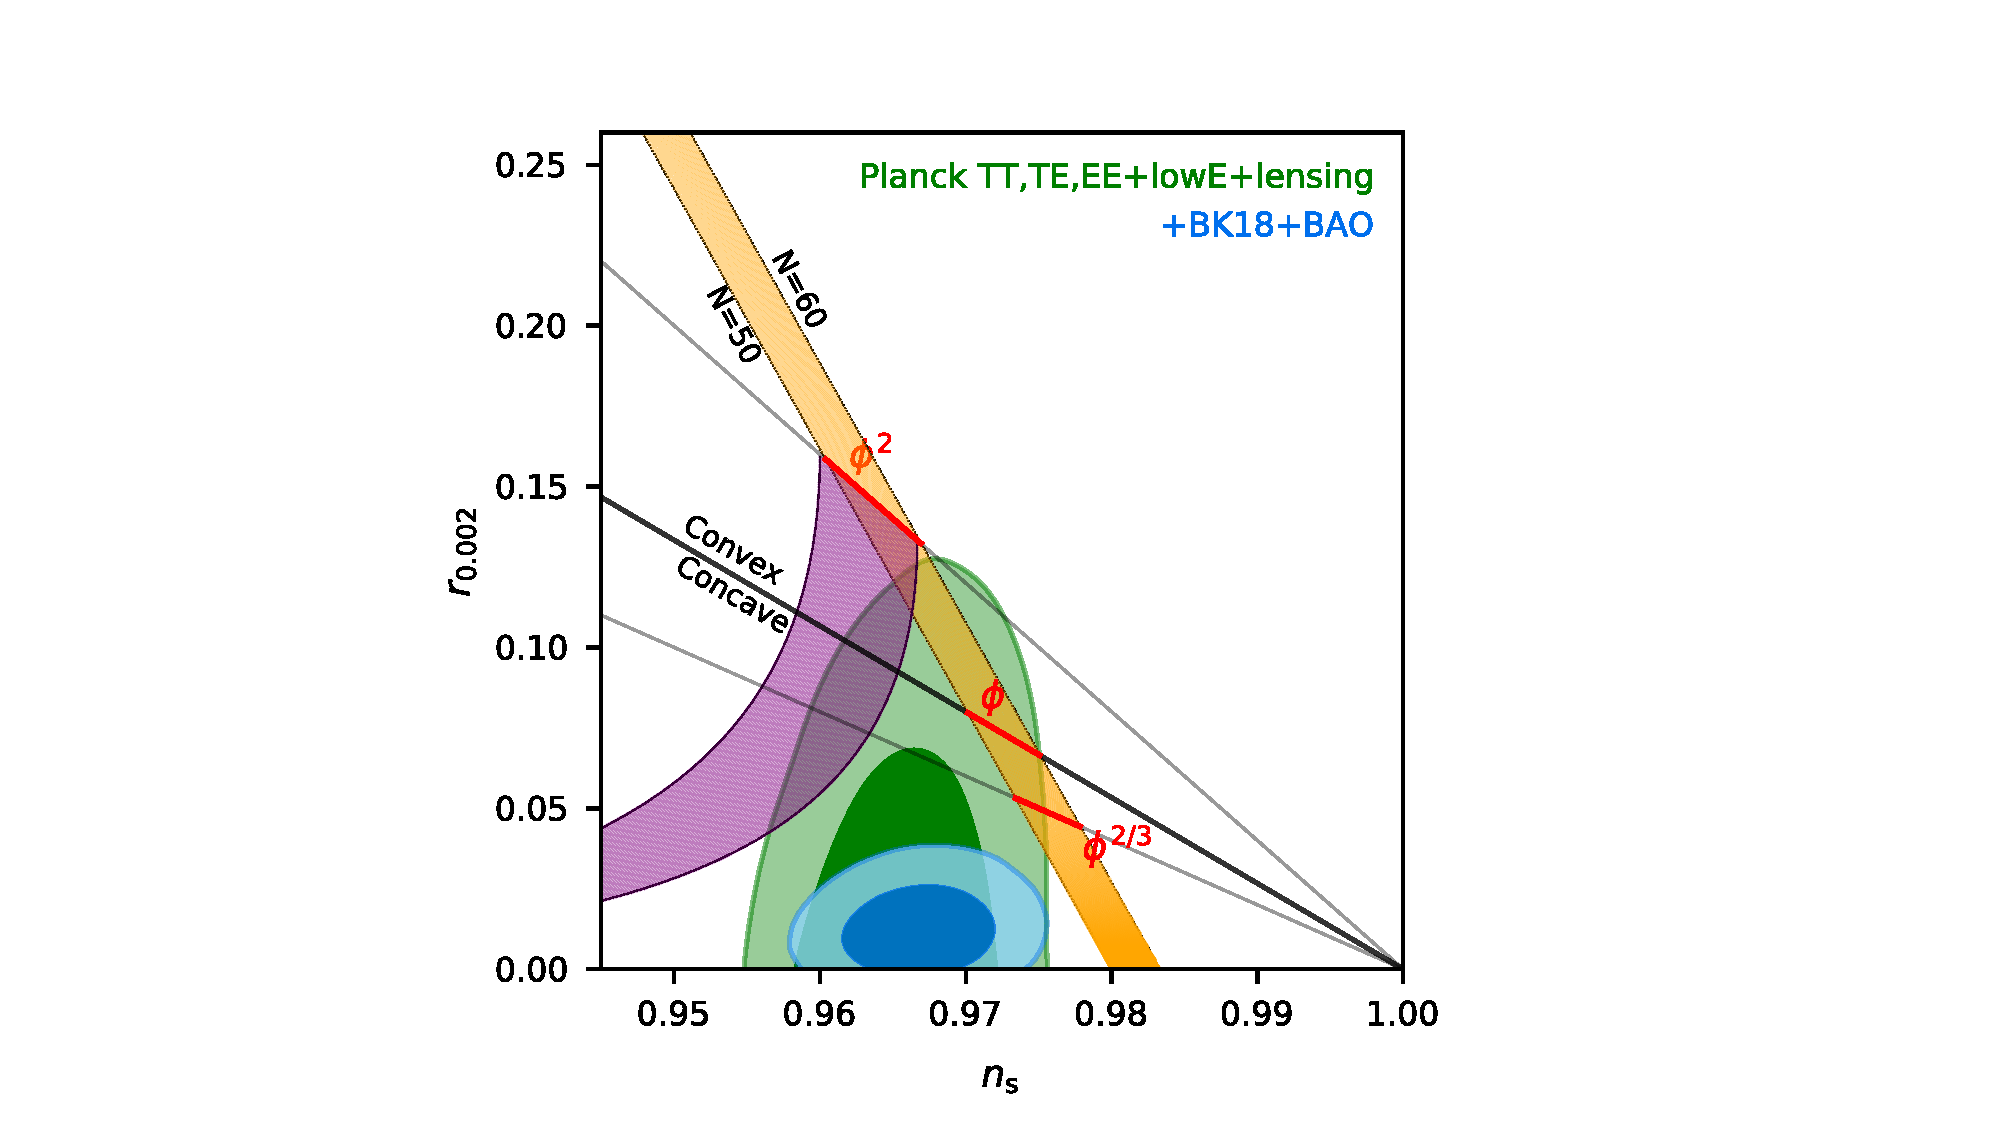
\includegraphics[width=140mm,height=85mm]{Sections/Figures/SpectralIndex.pdf} 
\caption{The most recent constraints on inflationary models in the tensor-to-scalar ratio $r$ and spectral index $n_s$ plane, taken from \cite{BICEP:2021xfz}. A substantial amount of inflationary models are already in tension with observations. } \label{Fig:SpectralIndex} 
\end{center}
\end{figure}



\subsection{Multi-field Inflation}
\label{sec:multinf}

So far, we have discussed the simplest (vanilla) inflationary scenario, where a single canonically normalised scalar field drives inflation. However, as discussed at more length in Sec. \ref{ModuliSection}, in string theory there are usually many scalar fields (as well as other fields of various spin) which may either drive inflation or act as spectator fields with interesting cosmological implications. In what follows, we briefly review these possibilities from a pure field theory perspective, which will be important for our discussion on string inflation in Sec. \ref{sec:infla}.

Let us consider the  Lagrangian for several scalar fields, minimally coupled to gravity\footnote{For a recent review on multi-field inflation in field theory see \cite{Gong:2016qmq}.}:
\be\label{4Daction}
S= \int{d^4x \sqrt{-\tt g} \left[\Mp^2 \frac{R}{2}  - \frac12\,g_{ab}(\phi^c) \partial_\mu\phi^a \partial^\mu\phi^b - V(\phi^a)\right]} \,,
\ee
where $g_{ab}$ is the {\em field space metric}.  The equations of motion derived from this action are given by
\bea
&&H^2 = \frac{1}{3\Mp^2} \left(\frac{\dot \varphi^2}{2}  + V(\phi^a)\right) \,, \label{H} \\
&& \ddot \phi^a + 3H\dot\phi^a + \Gamma^a_{bc} \dot\phi^b\dot\phi^c + g^{ab} V_{,b} =0  \,,
\label{phis}
\eea
where
\be\label{varphi}
\dot\varphi^2 \equiv g_{ab} \dot \phi^a\dot\phi^b\,
\ee
and the Christoffel symbols in \eqref{phis} are computed using the scalar manifold metric $g_{ab}$, while $V_{,a}$ denotes derivatives with respect to the scalar field $\phi^a$.



The slow-roll conditions and rapid turning in multi-field inflation  can be understood neatly  using a  kinematic basis to decompose the inflationary trajectory into {\em tangent} and {\em normal} directions  (i.e.~adiabatic and entropic). Focusing on the two field case for concreteness, we introduce   unit tangent (adiabatic) and normal (entropic) vectors  $T^a$ and $N^a$, as follows:
\be
T^a = \frac{\dot\phi^a}{\dot\varphi}\,, \qquad T^aT_a =1\,,\qquad
N^aT_a=0, \qquad N^aN_a=1\,.
\ee
The  equations of motion \eqref{phis} for the scalars $\phi^a$ projected along these two directions become:
\bea
 \ddot\varphi + 3H\dot\varphi + V_T & = &0 \,, \label{varphiT}\\
D_t T^a  + \Omega N^a &=&0\,,\label{varphiN}
\eea
 where $V_T = V_{,a}T^a$, $V_N = V_{,a}N^a$ and the {\em turning rate} parameter, $\Omega$, is defined as
\be\label{Omega}
\setlength\fboxsep{0.25cm}
\setlength\fboxrule{0.4pt}
\boxed{
\Omega \equiv \frac{V_N}{\dot\varphi}\,.}
\ee
The field-space covariant time derivative is  defined as:
 \be\label{Dt}
 D_tT^a \equiv \dot T^a + \Gamma^{a}_{bc} T^b \dot \phi^c \,.
 \ee

Using the equations of motion, we can  write  the projections of the Hessian elements along the tangent vector as  \cite{Achucarro:2010da,Hetz:2016ics,Christodoulidis:2018qdw,Chakraborty:2019dfh}:
\be\label{VTT1}
\frac{V_{TT}}{3H^2} =  \frac{\Omega^2}{3H^2} + 2\,\epsilon -\frac{\eta}{2} -
\frac{\xi_\varphi}{3}   \,,
\ee
as well as the projection along $T $ and $N$ as \cite{Aragam:2021scu}:
\be
\label{VTN1}
\frac{V_{TN}}{3H^2} = w\left( 1-\epsilon+\frac\eta3+\frac\nu3 \right).
\ee
In these equations  we  introduced  the slow-roll parameter
\be
\xi_\varphi\equiv \frac{\dddot\varphi}{H^2 \dot\varphi}\,,
\ee
as well as the {\em dimensionless turning rate}, $w$, which measures the {\em non-geodesicity} of the trajectory:
\be\label{eq:w}
\setlength\fboxsep{0.25cm}
\setlength\fboxrule{0.4pt}
\boxed{
w \equiv \frac{\Omega}{H}\,,}
\ee
and a new {\em slow-roll} parameter, which arises only in the multi-field case, $\nu$:
\be\label{eq:nu}
\setlength\fboxsep{0.25cm}
\setlength\fboxrule{0.4pt}
\boxed{
\nu\equiv \frac{\dot w}{H\,w}\,.}
\ee

\smallskip

\ni Note  that the expressions \eqref{VTT1}, \eqref{VTN1}  {\em are exact}, as we have not made use of any slow-roll approximations.
 On the other hand, $V_{NN}$ depends on the inflationary trajectory in a model-dependent fashion.

\subsubsection{Slow-roll in multi-field inflation}

Let us revisit the slow-roll conditions in the case that more than one field is present. These  require the  slow-roll parameters $\epsilon, \eta, \delta_\varphi $ above, to be much smaller than one in order to guarantee long-lasting, slow-roll inflation, that is,  $\epsilon, \eta, \delta_\varphi, \xi_\varphi \ll 1$. It is easy to check that these conditions imply
\bea
&&H^2 \simeq \frac{V}{3M_{Pl}} \,, \\
&& 3 H\dot \varphi + V_T \simeq 0 \,, 
\eea
and thus that the tangent projection of the derivative of the potential needs to be  small:
\be\label{epT}
\epsilon_T \equiv \frac{M_{Pl}^2}{2} \left(\frac{V_T}{V}\right)^2 \ll1  \,.
\ee
On the other hand, the normal projection $V_N$ can be large,  and it is related to the turning rate defined in eq.~\eqref{Omega}.
Moreover, from \eqref{VTT1} we see that during slow-roll, the equations of motion imply
\be\label{VTTsr}
\frac{V_{TT }}{3H^2} \sim \frac{\Omega^2}{3H^2}\,,
\ee
while from \eqref{VTN1}, requiring $\eta\ll1$ (equivalently $\delta_\varphi \ll 1$) implies that (barring possible cancellations)
\be\label{VTN_slowroll}
   \frac{V_{TN}}{3H^2}\sim \frac{ \Omega}{H} \,, \qquad {\rm and} \qquad
     \nu \ll 1\,.
\ee
Hence, we see that $\nu$ behaves as a new slow-roll parameter in multi-field inflation: the turning rate is guaranteed to be slowly varying during slow-roll \cite{Aragam:2020uqi,Aragam:2021scu}.

We see then that in the multi-field case, slow-roll inflation does not require small eigenvalues of the Hessian \cite{Chakraborty:2019dfh,Aragam:2021scu}, as usually believed. Namely, defining the multi-field generalisation of the $\eta_V$ parameter \eqref{eq:etaV} as
\be\label{etaVmulti}
\setlength\fboxsep{0.25cm}
\setlength\fboxrule{0.4pt}
\boxed{
\eta_V^{ m} \equiv \Mp^2 \left|{\rm min\,\,\, eigenvalue}  \left(\frac{ \nabla^a \nabla_b V}{V}\right)\right|, }
\ee
it is clear that $\eta_V^m$ does not need to be small and indeed can  be much  larger than one in multi-field inflation \cite{Chakraborty:2019dfh,Aragam:2021scu}. This implies that in multi-field inflation, all inflatons can be heavier than the Hubble scale \cite{Chakraborty:2019dfh}.
Thus the $\eta$-problem in multi-field inflation may manifest itself, if present, in a different form. For example, the curvature of the field space metric, $R_{\rm fs}$, may in general be non-zero and in particular could be large (in Planck units). Therefore, this introduces a new scale, and the flatness of the potential may be constrained over this new scale (see e.g.~\cite{Renaux-Petel:2021yxh}). However, in general, we expect $R_{\rm fs}$ to be of order one in Planck units.

\subsubsection*{ Multi-field inflation and swampland constraints}

Let us finally make some comments  between multi-field  inflation and the recently proposed dS conjectures \cite{Obied:2018sgi,Garg:2018reu,Ooguri:2018wrx}, which require that (see Section \ref{Sec:Swamp})
\bea\label{eq:swamp1}
 \frac{\nabla V}{V} \geq \frac{c}{\Mp}  \qquad {\text{or}}  \qquad %\\
  \frac{{\rm min} (\nabla^a \nabla_b V)}{V} \leq -\frac{c'}{\Mp^2},
\eea
where $c, c'$ are  ${\cal O}(1)$ constants.
From our discussion on  slow-roll inflation in the multi-field case, it can be easily seen that  the first condition in \eqref{eq:swamp1} can be satisfied, so long as the  turning rate $\Omega/H$  is sufficiently large \cite{Achucarro:2018vey}.
Indeed, the potential slow-roll parameter \eqref{eq:epsV} in  the multi-field case is given by
\be\label{epsimulti}
\epsilon_V^m \equiv \frac{\Mp^2}{2} \frac{V^aV_a}{V^2} = \epsilon_T + \frac{\Omega^2}{9H^2}\epsilon \,.
\ee
For $\epsilon_T\simeq \epsilon$,  one arrives at the relation  \cite{Achucarro:2018vey,Hetz:2016ics}:
\be\label{epsV2}
\epsilon_V^m \simeq \epsilon\left(1  + \frac{\Omega^2}{9H^2}\right)\,,
\ee
and therefore we see that in a multi-field inflationary model, where $\Omega\ne 0$, for sufficiently large turning rate  $\Omega/H$  $\epsilon_V^m$ can be comparable to or larger than one.
On the other hand, the second condition in \eqref{eq:swamp1} is precisely the requirement that $\eta_V^m$  be large (with negative eigenvalue). As we discussed above, this can happen in mulltifield slow-roll inflation without disrupting it\footnote{A field theory example with large values of $c'$ is given in \cite{Christodoulidis:2018qdw}. Supergravity examples with large $c'$ are given in \cite{Aragam:2021scu}.}.
In summary, multi-field inflation allows for  new inflationary attractors, which do not need to satisfy the single field potential flatness conditions \eqref{eq:epsV}, \eqref{eq:etaV}.



\subsubsection{Cosmological perturbations, the multi-field case}

The presence of more than one field changes the kinds of primordial fluctuations which are possible, because with several fields there can be perturbations,  for which the total energy density, $\delta\rho=0$, remains unchanged. Such fluctuations are called  {\em isocurvature} fluctuations, in contrast to the {\em adiabatic} fluctuations involving nonzero $\delta\rho$ considered in the single field case.

There are strong observational constraints on the existence of isocurvature fluctuations and current observations are consistent with purely adiabatic oscillations at horizon re-entry  \cite{Planck:2018vyg,Planck:2018jri}. Primordial isocurvature modes need not be a problem for an inflationary model even if they are generated at horizon exit, provided they are subsequently erased before horizon re-entry. Moreover, the presence of more than one field can give rise to large non-Gaussianties in the power spectrum, which are also constrained by observations \cite{Planck:2019kim}. At the same time, additional scalars -- as well as other higher spin fields -- may give rise to interesting phenomenology and are thus of great interest for future 
%
experiments\footnote{See \cite{Arkani-Hamed:2015bza,Lee:2016vti,Alexander:2019vtb} for studies  of the imprints of new (higher spin) particles on the non-gaussianities of the cosmological fluctuations and \cite{Alexander:2020gmv,Criado:2020jkp,Jenks:2022wtj,Gondolo:2021fqo} for proposals of dark matter as higher spin fields, and their phenomenology.
}.

\subsubsection{Spectator fields during inflation}

Scalar fields acting as spectators during inflation are well motivated not only from a purely field theory perspective, but also from a phenomenological point of view. Any additional fields may give rise to interesting features that could produce observable effects which would then be of great importance. The same can be said for spin one fields such as $U(1)$ vector fields, producing for example   anisotropies, as well as $SU(2)$ gauge fields, potentially sourcing  tensor perturbations, and evading the Lyth bound discussed above (see e.g.~\cite{Maleknejad:2012fw} for a review).
We will not review here the vast literature on the subject, but will mention some interesting possibilities in the context of string cosmology in Sec. \ref{sec:infla}.

\subsection{Quintessence}\label{sec:quint}

As we mentioned before (see Sec.~\ref{subsecME}),  current observations provide strong evidence for the current acceleration of the universe.
In the $\Lambda$CDM standard model of cosmology, this is due to a constant vacuum energy, $\Lambda$.
However, the constant vacuum energy appears to be  much smaller than  would be expected from estimates based on quantum field theory. This has led to the  widespread speculation that the vacuum energy may not be constant, but it may now be small because the universe is old. Such a  time-varying vacuum energy is called {\em quintessence} \cite{Wetterich:1987fm,Peebles:1987ek,Ratra:1987rm}.\footnote{The name quintessence was coined in \cite{Caldwell:1997ii}. For reviews and several references see e.g.~\cite{Copeland:2006wr,Linder:2007wa,Tsujikawa:2013fta}.}

The natural way to introduce a time-varying vacuum energy is to assume the existence of one or more scalar fields, on which the vacuum energy depends, and whose cosmic expectation values change with time. We have seen that scalar fields of this type  play a crucial role in cosmological inflation and thus the discussion of quintessence uses several of the concepts which already appear in inflation.
Considering a single scalar field, the idea is that its dynamics drive the present epoch of accelerated expansion. Dark energy started to dominate relatively recently, namely less than a single e-fold ago (see Fig.~\ref{fig:RhoEvol}). It may therefore seem easy to have a sufficiently flat scalar potential, which starts dominating the energy density less than an e-folding ago.
The original and simplest example is provided by the following potential \cite{Wetterich:1987fm,Peebles:1987ek,Ratra:1987rm}
\be
\label{eq:QV}
V(\phi) = M^{4+\alpha} \phi^{-\alpha},
\ee
where $\alpha$ is positive but otherwise arbitrary, and $M$ is a constant with units of mass. We can call this type of potential  {\em runaway} like. We give a brief discussion here, but explore this class of runaway potentials in string theory more in Sec. \ref{reheating} and Sec. \ref{sec:DE}, in the context of both transient post-inflationary runaways and also quintessence dynamics in the late-time universe. 
The model \eqref{eq:QV} can be solved in some detail as a concrete example of quintessence (see e.g.~\cite{Weinberg:2008zzc} and further discussion in Sec. \ref{sec:DE}).

Any successful quintessence must have the property that at early times, the energy density of the quintessence field is subdominant over radiation to avoid conflict with BBN. With potential \eqref{eq:QV}, one can show that the field has a solution at early times during radiation domination such that
\be
\rho_\phi\propto t^{-2\alpha/(\alpha+2)}\,,
\ee
and thus at early times ($t\ll 1$) $\rho_\phi$ is indeed less than $\rho_r$ which goes as $t^{-2}$. This solution turns out 
to be an attractor, known as a {\em tracker solution}. After radiation domination, the universe undergoes an epoch of matter domination, but the tracker solution of $\phi$ continues to have energy density falling as $\rho_\phi\sim t^{-2\alpha/(\alpha+2)}$, and since $\rho_r$ and $\rho_m$ decrease faster ($t^{-8/3}, t^{-2}$ respectively in matter domination) eventually, both will fall below $\rho_\phi$. 

At late times, 
one finds $\rho_\phi\propto t^{-\alpha/(2+\alpha/2)}$, or $\ln a \propto t^{2/(2+\alpha/2)}$ and the expansion is  dominated by the quintessence field.  The point when $\rho_m=\rho_\phi$ is given by
$t_c\approx M^{-(4+\alpha)/2}G_4^{-(2+\alpha)/4}$, which gives $\phi(t_c)\approx G_4^{-1/2}$. 
Finally, to achieve agreement with observations, setting the critical time $t_c$ at which $\rho_m\approx \rho_\phi$ to be close to the present moment $t_0 \approx 1/H_0$,  requires the constant factor in $V(\phi)$ to take the value
\be
M^{4+\alpha} \approx G_4^{-1-\alpha/2}H_0^2\,.
\ee
There is, however, no fundamental explanation as to why this should be the case.

Although quintessence has been proposed as a potential candidate to explain the current acceleration, it still faces several challenges. We will discuss later on  in more detail how these manifest  in the context of string theory (see Sec.~\ref{sec:ChallengesQ}), but let us briefly mention here some of the main challenges for any model of quintessence.
\bi
 \item {\em Fine-tunings}. As can be evident from the above discussion, quintessence models need to explain why the field has to be exactly at the point where $V(\phi_0) \simeq \rho_0 \simeq (0.003 \,{\rm eV})^4$ today. Moreover, it is not hard to check that a successful quintessence model requires the mass of the field to be extremely light, $m_\phi\simeq H_0\simeq 10^{-33}\,{\rm eV}$ (at least in the case of single field), which must be protected against quantum corrections.

\item {\em Phenomenological constraints}. Phenomenological problems to realise quintessence arise as the quintessence field must be extremely weakly coupled to ordinary matter;  otherwise, its exchange would generate observable long-range forces, which are severely constrained by experiments.
The quintessence field can be a scalar as we saw above, or a pseudoscalar, such as an axion.\footnote{Other fields have also been proposed as quintessence, however the same problems arise as for the scalar case.} The advantage of axions is that they can avoid  fifth-force constraints, but a typical axion potential requires a trans-Planckian decay constant to drive any successful period of accelerated expansion.
\ei


\subsection{Possible Tensions with $\Lambda$CDM?}

We end this overview section on cosmology with mention of various possible hints towards tensions between Planck observations of the CMB and other cosmological probes.  Although the statistical significance of these tensions is not definitive, and even still under debate, if any are confirmed and not due to systematics, this would be exciting evidence of new physics beyond the $\Lambda$CDM model.  

The most famous of these tensions is the Hubble tension.  Planck constraints on today's Hubble parameter, which is obtained by assuming the standard six parameter $\Lambda$CDM model, yields $H_0 = 67.44 \pm 0.58 {\rm km}\,{\rm s}^{-1}\,{\rm Mpc}^{-1}$ \cite{Planck:2018vyg}.  This is to be contrasted with recent direct local distance ladder measurements of $H_0$ from the SH0ES collaboration, which gives instead $H_0 = 74.03 \pm 1.42 {\rm km}\,{\rm s}^{-1}\,{\rm Mpc}^{-1}$ \cite{Riess:2019cxk}. This amounts to a $4.3\sigma$ discrepancy, with other direct measurements going in the same direction.  For a recent review on the $H_0$ discrepancies and phenomenological solutions see \cite{DiValentino:2021izs}; see \cite{Efstathiou:2020wxn} for a critical perspective. Proposals to resolve the tension include increasing the number of effective neutrino species $N_{\rm eff}$, modifying the dark energy equation of state, and the presence of some early dark energy; for a systematic comparison of several proposals and their relative success see \cite{Schoneberg:2021qvd}.  A review of all the current discordances, covering $H_0$, the $\sigma_8$--$S_8$ tension, and other less statistically significant anomalies, together with an experimental outlook, is given in \cite{Abdalla:2022yfr}.

\enddocument


\newpage


\input{Sections/ModuliFQV2}

\input{Sections/InflationNewV2}

\input{Sections/PostinflationNewV2}

\section{Dark Energy}
\label{sec:DE}

As we discussed in Sec. \ref{SecCO}, one of the most striking discoveries from the last century was the observational discovery of late-time cosmic acceleration from Type IA Supernovae (SN Ia) \cite{Riess:1998cb,Perlmutter:1998np}. This discovery represents one of the major puzzles of modern physics; its cause is generally dubbed {\em dark energy}, whose fundamental nature is still a mystery. According to observations, about $70\%$ of the energy density of the universe today consists of this unknown dark energy component. This has also been confirmed by other observations -- e.g. through Cosmic Microwave Background (CMB) \cite{WMAP:2003elm,Planck:2018vyg} or Baryon Acoustic Oscillations (BAO) \cite{SDSS:2005xqv} (however, see \cite{Sarkar:2007cx} for a dissenting view). 

Dark energy is characterised by an equation of state (see Sec.~\ref{SecCO})
\begin{equation}
\setlength\fboxsep{0.25cm}
\setlength\fboxrule{0.4pt}
\boxed{
w_{\rm DE} = p_{\rm DE}/\rho_{\rm DE} \,, \quad {\text{with}} \quad w_{\rm DE}< -1/3.
}
\end{equation}
Present observations suggest that the current energy density of dark energy is
$\rho_{{\rm DE}, 0} \sim 10^{-120}\,M_{\rm Pl}^4$, with an equation of state parameter given today by \cite{Planck:2018vyg}:
\begin{equation}
\setlength\fboxsep{0.25cm}
\setlength\fboxrule{0.4pt}
\boxed{
w_{{\rm DE}, 0} = -1.03 \pm 0.03 \,.
}
\end{equation}
 
The simplest candidate for dark energy, consistent with current data and used in the $\Lambda$CDM cosmological model, is a pure cosmological constant, $\Lambda$,  with $w_{\rm DE} =-1$. The cosmological constant can arise from the vacuum energy in particle physics, but the naive theoretical expectation for this is about $120$ orders of magnitude larger than the observed value \cite{Weinberg1}. 
To explain the extremely fine-tuned value of the cosmological constant, one possibility is to appeal to anthropic arguments  \cite{Weinberg2,Garriga:1999bf}, whose recent resurgence is motivated by the string theory landscape \cite{Douglas:2006es}. 

An alternative possibility is that the cosmological constant actually vanishes for reasons yet to be understood, calling for an alternative mechanism to explain the origin of dark energy.  The observations that constrain the value of $w_{\rm DE}$ today to be close to minus one (the value for a 
pure cosmological constant) say relatively little about its time evolution (see \cite{Planck:2018vyg} for constraints on a time-dependent equation of state parameter, using the phenomenological parameterisation $w = w_0 + (1-a)w_a$). So we can consider a situation in which the dark energy equation of state parameter changes with time, similarly to what happens during early universe inflation. As scalar fields naturally arise in supergravity and string theory, there are plenty of potential candidates for dark energy. Indeed, as we will see, many of the ideas discussed in Sec. \ref{sec:infla} to explain cosmic inflation from string theory can also be applied to the late-time cosmic acceleration. On the one hand, as only around a single e-folding of accelerated expansion is needed for dark energy, compared to $60$ e-foldings for inflation, constructing models of dark energy is easier. On the other hand, as dark energy is active today, it is constrained more strongly by  experiments and observations as well as by theoretical challenges as discussed in Sec.~\ref{sec:quint}.

We now consider recent developments using these two approaches to explain the current accelerated expansion of the universe within the context of string theory and string-inspired constructions.\footnote{For recent reviews see \cite{Berglund:2022qsb, Dutta:2021bih}.}

\subsection{Dark Energy as Vacuum Energy}

In this section we review the cosmological constant problem and the order of magnitude estimates of the vacuum energy.  We then describe how the string theory multiverse, using eternal inflation to populate it, has the potential to solve the cosmological constant problem, providing a (controversial) framework in which the fine-tuning of the vacuum energy is explained via anthropic arguments. Finally, we discuss the main questions that this paradigm leaves open.

\subsubsection{The cosmological constant problem}

The modern formulation of the cosmological constant problem actually raises two questions (see  \cite{Weinberg1, Carroll:2000fy, Padmanabhan:2002ji, Martin:2012bt, Li:2012dt, Burgess:2013ara,Padilla:2015aaa} for some reviews and \cite{Straumann:2002tv} for a historical account):
\begin{itemize}
\item Why is the cosmological constant so small but non-zero? 
\item The Coincidence Problem: why is the cosmological constant today comparable to the matter energy density today?
\end{itemize}
Phase transitions (as illustrated for bubble nucleation in figure \ref{fig:BubbleNucleation}) through the cosmological history would have changed the total vacuum energy, so any solution to the problem needs to ensure that the vacuum energy is suppressed throughout.  However, what makes the cosmological constant problem most challenging is that it is a low-energy problem, which can be posed at scales which we believe we understand very well. For instance, summing up vacuum-loop diagrams to a cutoff $M\sim 100$ GeV -- a reasonable scale given the success of the Standard Model in accelerator experiments -- the electron contributes:
\begin{equation}
\rho_e \sim \mathcal{O}\left(M^4\right) + \mathcal{O}\left( M^2 m_e^2 \right) + \mathcal{O}\left( m_e^4\ln \frac{M}{m_e}\right) \,,
\end{equation}
which is already around $55$ orders of magnitude too large. A recent estimate of the total vacuum energy from the Standard Model of particle physics, using a Lorentz invariant renormalisation scheme, gives a value for the energy density today of $\rho_\Lambda \sim -3.2 \times 10^8$ GeV$^4$ \cite{Koksma:2011cq,Martin:2012bt}. It is important to note that the gravitational effect of quantum loops has been experimentally observed \emph{in matter}; they are known to contribute to the inertial mass of particles via the Lamb shift and the nuclear electrostatic energy, where the equivalence principle has been verified to at least one part in a million \cite{Polchinski:2006gy}. Nonetheless, cosmological constraints on the vacuum energy would seem to indicate that quantum loops \emph{in the vacuum} do not gravitate. Although the length scale of the cosmological constant problem is huge, $H_0^{\;-1}$, as it occurs precisely at the point that quantum physics meets gravity, we might hope that a better understanding of string theory will offer a solution.

\begin{figure}[ht]
\centering
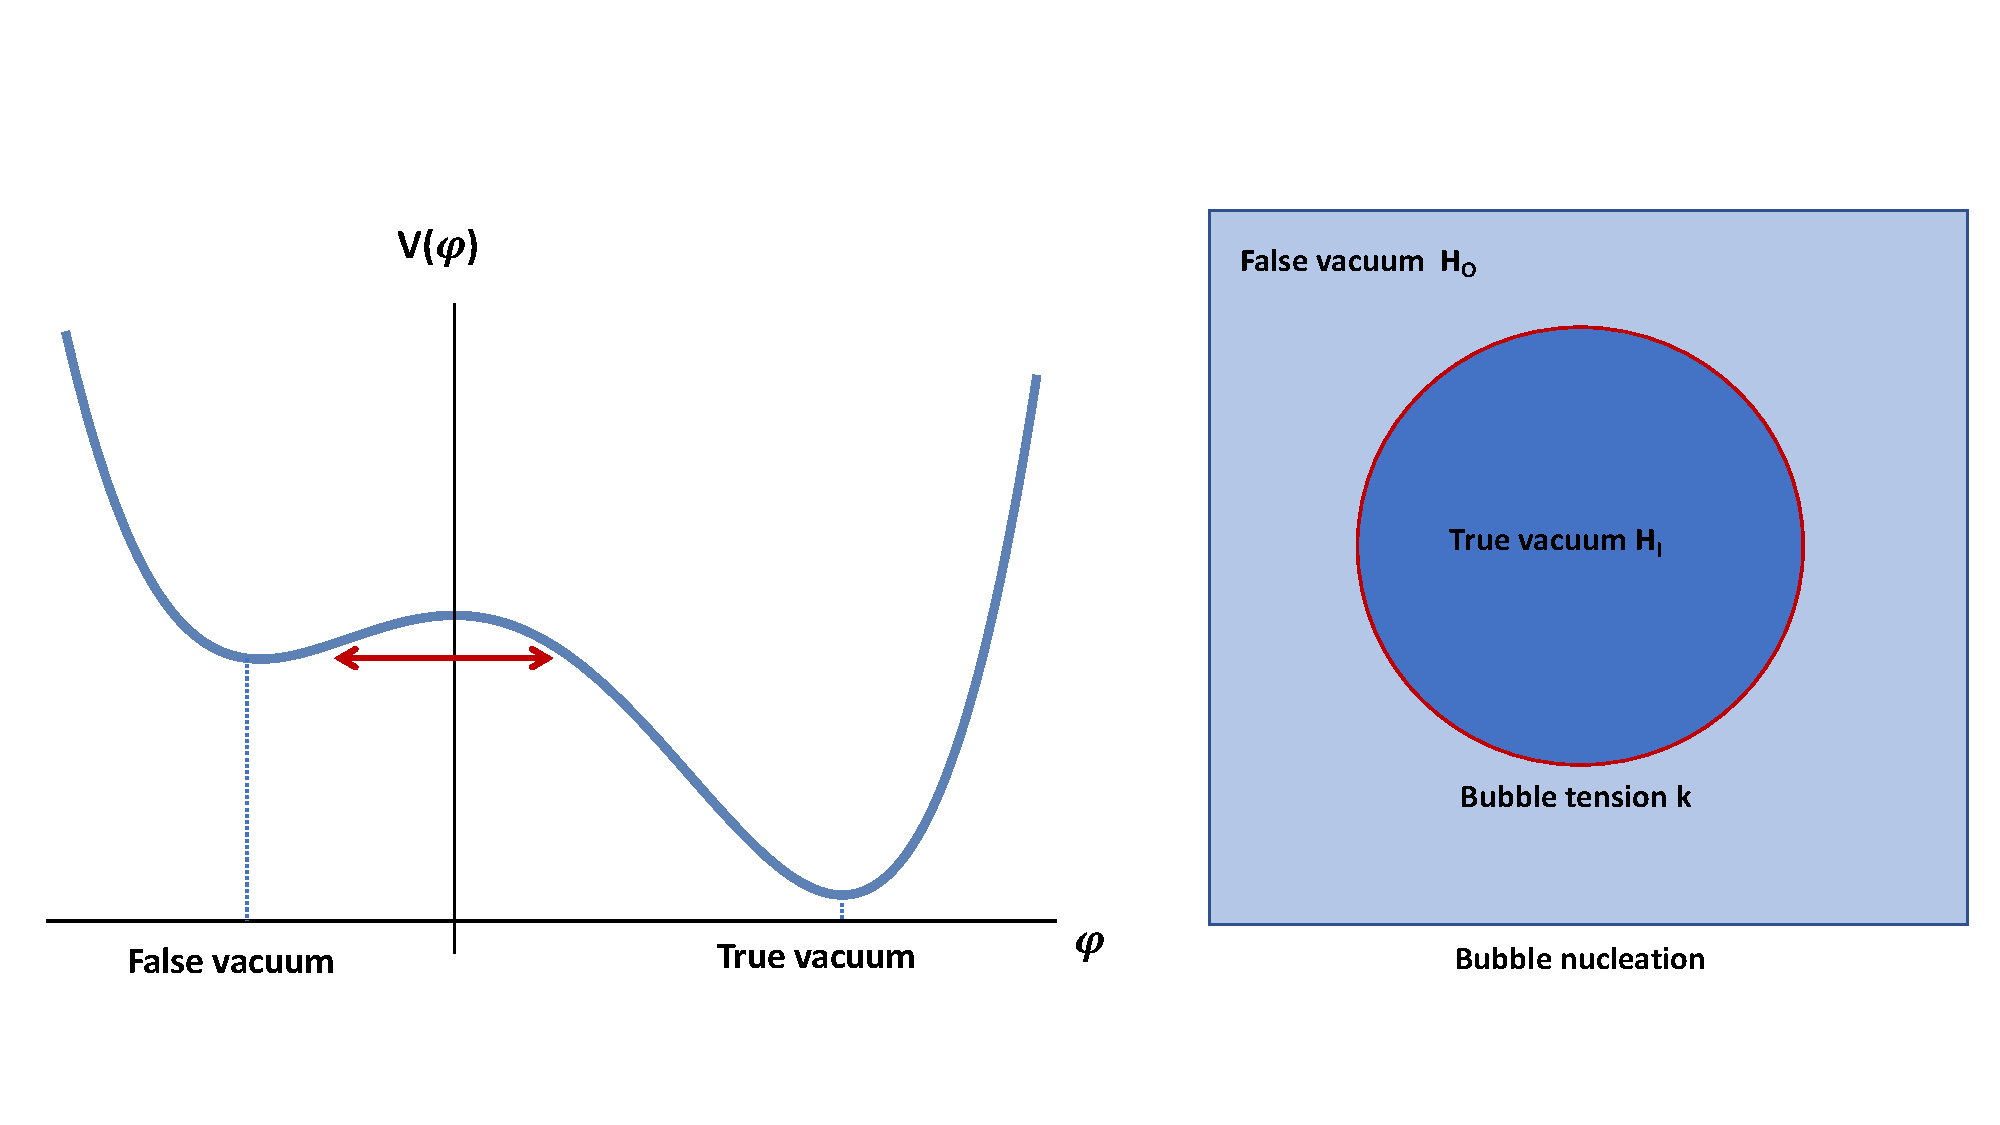
\includegraphics[width = 0.9\textwidth]{Sections/Figures/VacuumTransition.pdf} 
\caption{Bubble nucleation for a transition from a false to a true vacuum. The opposite transition is also allowed as long as the two spaces are dS.}
\label{fig:BubbleNucleation}
\end{figure}

\subsubsection{The anthropic principle and the string theory landscape}
\label{ssec:landscape}

Even without any microscopic understanding to hand, our very existence suggests that the cancellation of vacuum energy has to occur. If the vacuum energy were positive and much larger than the observed value, the growth of structure would have ceased too early preventing the formation of galaxies. If it were much larger and negative, the universe would have already collapsed in a Big Crunch. Remarkably, Weinberg \cite{Weinberg2} arrived at the \emph{prediction} that the vacuum energy must be small and of the same order as the matter energy density using this anthropic argument with bound:\footnote{Although note that cosmological constants much larger than the observed value were already known to be excluded.}
\begin{equation}
\setlength\fboxsep{0.25cm}
\setlength\fboxrule{0.4pt}
\boxed{
-10^{-123} M_{\rm Pl}^4 \lesssim \rho_\Lambda \lesssim 3 \times 10^{-121} M_{\rm Pl}^4 \,. 
}
\label{E:Weinwin}
\end{equation}
If one assumes that observers require galaxies, and that observers typically evolve soon after galaxy formation, then the \emph{Why Now?} problem is also solved, as allowing the vacuum energy to be as large as possible whilst allowing for galaxy formation places it in line with the matter energy density directly after galaxy formation.  For the argument to be complete, one also requires a theory to produce a multitude of vacua, including ones with anthropically viable total vacuum energies, and a mechanism to populate them all. This is what the string theory landscape \cite{Susskind:2003kw} is proposed to provide.

As reviewed in Sec. 3, string theory has a (probably finite \cite{Douglas:2003um, Ashok:2003gk} but) enormous number of solutions corresponding to 4-dimensional spacetimes at low energies, which we call the \emph{string theory landscape}. Each solution has a number of distinct contributions to the vacuum energy.  The value of the moduli potential energy discussed in Sec. 3 (which incorporates classical and leading order perturbative and/or non-perturbative effects) is one such contribution. To these should be added subleading quantum corrections in both the $g_s$ and $\alpha'$ expansions, amongst which those at $\mathcal{O}(\alpha'^0)$ incorporate standard field theory loops. By considering a string-inspired simplified model of such a setup, Bousso and Polchinski \cite{Bousso:2000xa} argued that the string theory landscape accommodates a discrete set of total vacuum energies that are sufficiently densely packed in Planck units to include the observed dark energy, and that moreover, all the corresponding vacua can be populated via an eternal inflation driven by non-perturbative bubble nucleation.

The discreteness of the distribution of vacuum energies arises from the topological nature of the input parameters for string compactifications -- flux quanta, D-brane and other localised source numbers, and an internal manifold characterised by its Hodge numbers -- which all contribute directly and indirectly to the vacuum energy.  Building on earlier work by Abbott \cite{Abbott:1984qf} and Brown and Teitelboim \cite{Brown:1987dd,Brown:1988kg}, Bousso and Polchinski \cite{Bousso:2000xa} (see also \cite{Bousso:2007gp} for a review) considered in particular the vacuum energy contribution from a set of $J$ 4-form background fluxes. In analogy to the electromagnetic field, each 4-form field-strength, $F_{(i)}$, is quantised in units of its source membrane's `electric'-charge $q_i$, $F_{(i)}^{mnpq} = n_i q_i \epsilon^{mnpq}$, and gives a positive vacuum energy contribution
\begin{equation}
\rho_{\rm 4-form} = \frac12 \sum_{i=1}^J n_i^2 q_i^2 \,.
\end{equation}
Crucially, the background 4-form fluxes are unstable to non-perturbative tunnelling effects described by Euclidean instantons, in analogy to how an electric field between two oppositely charged parallel capacitor plates discharges via Schwinger pair creation of electron and positrons, in the case of a 4-form, the depletion occurs via the spontaneous appearance of spherical membranes. Inside the membrane, the associated field strength is lowered by one unit of membrane charge: $n_iq_i \rightarrow (n_i-1)q_i$, with a subsequent reduction in energy, $(n_i-\frac12)q_i^2$ balanced by the initial mass of the membrane, which then expands outwards at the speed of light; see Fig. \ref{fig:BubbleNucleation}.  If one separates the total vacuum energy into the 4-form flux contributions and all the rest (which we may call the `bare' cosmological constant),
\begin{equation}
\rho_{\Lambda} = \lambda + \frac12 \sum_{i=1}^J n_i^2 q_i^2\,,
\end{equation}
it takes an exponentially long time for the
the background fluxes to deplete and so their vacuum energy contribution could eventually cancel an order one bare cosmological constant, $\lambda<0$, to give a total $\rho_\Lambda$ within the Weinberg window (\ref{E:Weinwin}).  This fine cancellation requires:
\begin{equation}
2|\lambda| \lesssim \sum_{i=1}^J n_i^2 q_i^2 \lesssim 2(|\lambda| + 10^{-118})\,.
\end{equation}
That this is possible for charges not much less than one relies on the fact that there are multiple distinct 4-form fluxes and associated membranes (see Fig. 1 from \cite{Bousso:2000xa}). These arise from M/string-theory compactifications as high-dimensional forms and branes, such as 5-branes wrapping distinct 3-cycles in the internal space. For example, an internal manifold with $\sim 500$ 3-cycles, with flux numbers ranging up to say $9$, would give $\sim 10^{500}$ different vacua for the construction. 

Whilst the Bousso-Polchinski toy model captures much of the physics of the landscape, realistic string constructions require further considerations \cite{Denef:2007pq}: moduli have to be stabilised; fluxes backreact on the geometry so that the bare cosmological constant $\lambda$ and charges $q_i$ themselves depend on the flux integers, leaving the cosmological constant to vary in unpredictable ways; the types and numbers of fluxes and branes that can be included are constrained by charge conservation or tadpole cancellation.  More sophisticated studies of the distributions of supersymmetric and non-supersymmetric Calabi-Yau flux compactifications of various string theories were carried out in \cite{Denef:2004ze, Douglas:2003um, Ashok:2003gk, Dienes:2006ut}. A recent development in this direction is the incorporation of K\"ahler moduli stabilisation, thereby ensuring that the sampling is only over the minima of the moduli potential (see e.g. \cite{Broeckel:2020fdz, Cicoli:2022chj} and references therein). Constructions with as many as $10^{272\,000}$ vacua have been proposed \cite{Taylor:2015xtz}, while F-theory models of dark energy have been proposed in \cite{Heckman:2019dsj, Heckman:2018mxl}.

In summary, string theory plausibly contains a landscape of vacua with a dense spectrum of vacuum energies that includes the observed vacuum energy, and a mechanism to populate them via membrane nucleation. The cosmological history of this scenario assumes that the universe starts with a large positive vacuum energy, expanding exponentially as dS space.  Eventually, somewhere within the universe, a membrane bubble will nucleate within which there is a lower vacuum energy.  This bubble will grow, but not as fast as the initial vacuum expands, the latter providing an ambient `multiverse'. Thus a process of eternal inflation ensues, with bubble nucleation continuing inside and outside existing bubbles, each bubble containing a long-lived open FRW universe and each jump in vacuum energy being not much smaller than one in Planck units, allowing for the creation of hot and dense universes. Eventually, one such bubble nucleation will create an anthropic universe, with the vacuum energy lowered to within the Weinberg range (\ref{E:Weinwin}) where the Big Bang begins.  See Fig. \ref{fig:Multiverse}.


\begin{figure}[ht]
    \centering
    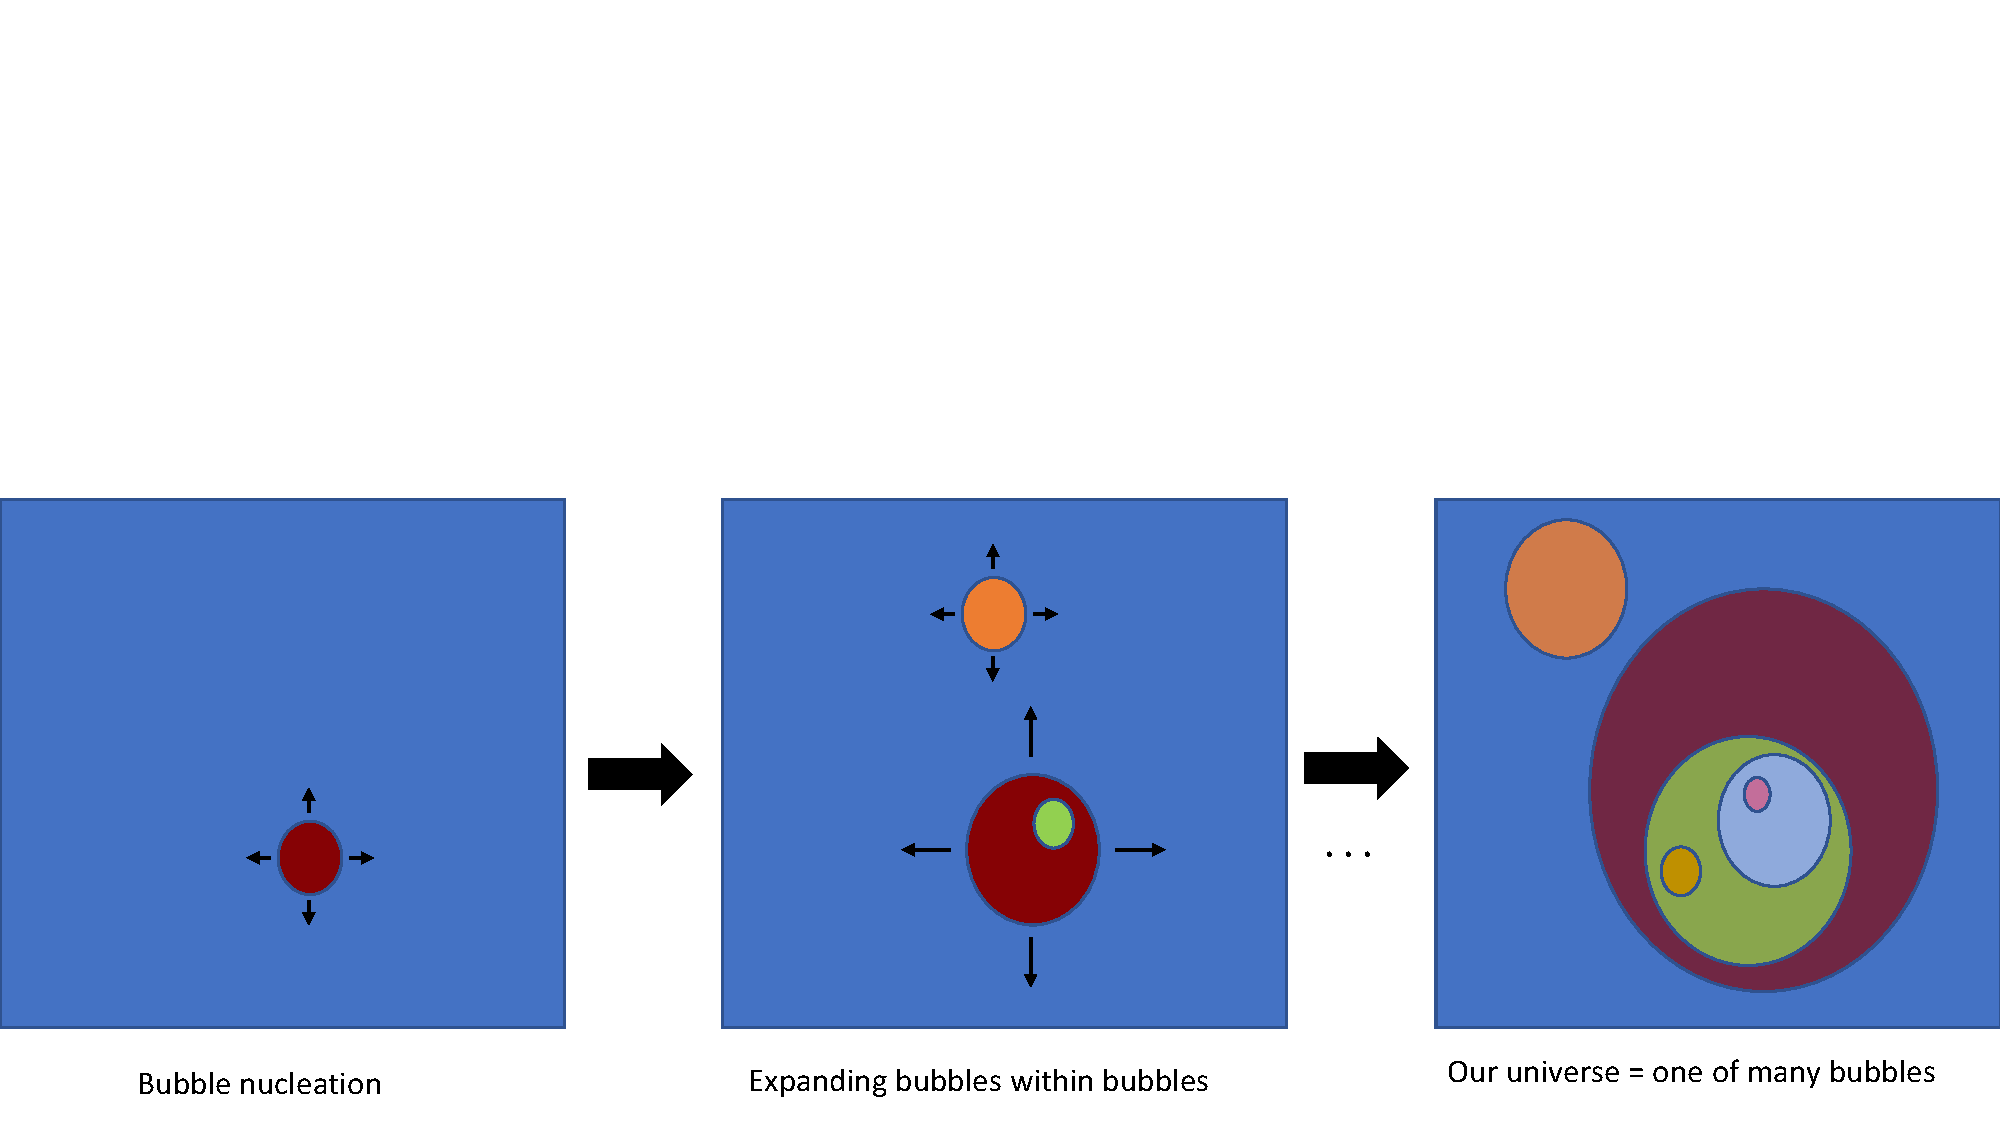
\includegraphics[width = 0.99\textwidth]{Sections/Figures/Figure_Multiverse_3.pdf} 
    \caption{Multiverse obtained by the process of bubble nucleation due to vacuum transitions from one dS vacuum to another with different cosmological constant.}
    \label{fig:Multiverse}
\end{figure}

\subsubsection{Open questions on the landscape}

The proposal of the string theory multiverse is deeply controversial. If true, it would motivates a paradigm shift in answer to the cosmological constant problem -- the value of the cosmological constant is environmental and our very existence implies it must happen to fall within the Weinberg range in our patch of the multiverse. In this case, there seems no reason to expect any further microscopic explanation at play. However, there remains work to be done.

Essential to the string theory landscape is an understanding of moduli stabilisation, reviewed in Sec. \ref{sec:MS}. So far, there are few attempts at achieving simultaneously moduli stabilisation and the Standard Model of particle physics (see \cite{Cicoli:2021dhg} for some recent progress). A complete model must (of course) include the vacuum energy of the Standard Model and dark matter amongst all the different contributions to be anthropically cancelled. 

To be more concrete, however, consider the simplified type IIB moduli stabilisation scenarios of KKLT and LVS. It is important to recognise that, although we can aim to make well-controlled dS vacua and -- remarkably -- even compute to good precision the vacuum energy in the weak coupling, weak curvature expansions, we cannot hope -- with current technology -- to obtain an explicit construction with fine-tuned vacuum energy $\mathcal{O}(10^{-120})$. The interplay between various classical and quantum effects are argued to give rise to metastable dS vacua, with the effective parameters such as $W_0$, $A$ and $a$ in $W =W_0+ A \, e^{-aT}$ (see Sec.~\ref{sec:MS}), ultimately depending on topological numbers such as flux integers and numbers of branes or instantons. The first obstacle arises from the difficulty to determine the exact dependence of parameters like $W_0$ and $A$ on the complex structure moduli and the explicit stabilisation of these moduli in terms of the discrete microscopic parameters. Moreover, even if discretely adjusting these integers allowed the effective parameters to be finely-tuned to give an anthropically viable metastable vacuum at weak coupling and large volume, the fine-tuning would typically be spoilt by higher order $g_s$ and $\alpha'$ corrections to the vacuum energy. To illustrate this point with a very simple toy model, consider a one-modulus system with canonical kinetic term and a scalar potential using an expansion in small $\phi$:
\begin{equation}
V(\phi) = \left(a_0 + a_2 \phi^2 + a_3 \phi^3 + a_4 \phi^4 + \dots\right)  \,.
\end{equation}
Assuming some mild hierarchy in the parameters $|a_3| \gg |a_i|$, $i\neq 3$, and $a_2 <0$, induces a metastable minimum $\langle \phi \rangle = -\frac{2 a_2}{a_3} \ll 1$ consistent with the expansion. If we assume that the leading coefficients are fine-tuned such that 
$$a_0-\frac{4}{27}\left(\frac{|a_2|^3}{a_3^2} \right) \sim 10^{-120},$$ 
then without further fine-tuning the higher order contributions $\mathcal{O}\left( \phi^4 \right)$ to the vacuum energy will dominate. Thus it is the full vacuum energy, including Standard Model/dark matter contributions and all $g_s$ and $\alpha'$ corrections -- right up to the order where the corrections are suppressed down to $10^{-120}\,M_{\rm Pl}^4$ without fine-tuning --  that has to be anthropically fine-tuned. This arguably weakens the significance of the challenges in uplifting the leading order AdS vacua of moduli stabilisation scenarios to dS (see \cite{deAlwis:2021zab}), although notice that the Standard Model contributions to the vacuum energy were found to be negative in \cite{Koksma:2011cq,Martin:2012bt}. Nevertheless, the key that the string landscape offers is the realisation that flux vacua lead to a finely-spaced distribution of vacuum energies over a suitably large range; even if the other contributions move this distribution up or down in energy, one may still expect vacuum energies of order of the observed dark energy amongst the final vacua.

Weinberg's anthropic window was derived by assuming that all other Standard Model parameters are fixed to their observed values. However, the string landscape suggests that all of these parameters would similarly vary from vacuum to vacuum.  For example, if effective field theory parameters are such that primordial density perturbations are larger or grow faster, anthropic arguments would require a larger positive vacuum energy. It is not yet clear how to use this framework to make predictions. Any statistical approach (see \cite{Denef:2004ze, Douglas:2003um, Broeckel:2020fdz, Broeckel:2021dpz, Cicoli:2022chj} and \cite{Kumar:2006tn} for a pedagogical review), by searching for those properties which have probability $\sim\mathcal{O}(1)$ in the landscape (see \cite{Page:2007bt, Hartle:2007zv} for discussions for and against our typicality) or identifying distinct low-energy features that are strongly correlated, would require an understanding of the measure on the space of vacua. Such a measure would need to include consideration of the dynamical mechanism that populates the landscape, which may prefer some vacua over others. This connects to the measure problem of eternal inflation, where bubbles of open universes with infinite spatial extent, reproduced infinitely many times, pose ambiguities in how to regularise \cite{Linde:1993xx, Guth:2000ka}.  

For some recent progress on searching the string landscape for models with phenomenological features using machine learning techniques see \cite{Cole:2021nnt}. Another strategy is to understand which classes of effective field theory can be consistently embedded into the string theory landscape (i.e. have a consistent UV completion into quantum gravity), and which classes instead lie in the swampland with no UV completion incorporating gravity \cite{Vafa:2005ui}. In fact, there are several conceptual challenges posed by any quantum theory on dS spacetime \cite{Witten:2001kn, Banks:2012hx, Maltz:2016iaw, Dvali:2018jhn}, most notably the absence of a well-defined S-matrix. Together with the technical challenges in achieving explicit, well-controlled moduli stabilisation with metastable dS vacua, this has led to the provocative conjecture that long-lived metastable dS vacua may actually lie in the swampland \cite{Garg:2018reu,Ooguri:2018wrx}. Although `may' does a lot of work in this last sentence, even if such a conjecture were true, it may still be of course reasonable to expect that our observed universe is sufficiently short-lived to stay in the landscape.

The landscape's approach to dark energy has led to several general proposals for combining it with the physics of vacuum transitions, a period of inflation, bubble collisions, etc. In particular, the general claim  that CDL vacuum transitions give rise to open universes after bubble nucleation has given rise to a holographic scenario for eternal inflation. See for instance \cite{Freivogel:2006xu,Sekino:2009kv}. For recent discussions to address the vacuum selection in terms of self-organised criticality see \cite{Kartvelishvili:2020thd,Giudice:2021viw}.

\subsection{Dynamical Dark Energy/Quintessence in String Theory}

In the previous section we discussed dS vacua in the string theory landscape as a possible explanation to present day accelerated expansion of the universe. However, given the debates around this proposal and observational prospects of measuring the dark energy equation of state and its time dependence, it is important to consider alternatives. The main alternative to a vacuum energy is a scalar field that is slow-rolling at positive energies, thus driving the accelerated expansion. This scenario goes under the generic name of {\em quintessence} \cite{Ratra:1987rm,Caldwell:1997ii} and much of the physics is similar to that of cosmic inflation, discussed in Sec. 4.
During quintessence, the equation of state of dark energy changes with time, similarly to inflationary cosmology, though initially Hubble friction can keep the field frozen yielding an effective cosmological constant. Quintessence scenarios with exponential or inverse power-law potentials are particularly attractive because they lead to equations of motion with attractor behaviour \cite{Ratra:1987rm} such that the present-day accelerated expansion is independent of the initial conditions. Moreover, these attractor solutions are usually scaling solutions such that the energy density scales as a power of the scale factor, and -- for the inverse power-law potentials -- the scalar field energy density can scale more slowly than the background fluid, allowing it to dominate eventually and drive the accelerated expansion \cite{Liddle:1998xm}.
 
Scalar fields abound in string theory and so it might seem rather natural to expect that one of them is at present rolling towards its minimum at a finite or infinite value. Among the scalar fields present in string theory, we can identify several potential candidates for quintessence: closed and open string string moduli, axions and runaway moduli. Moreover, scenarios where more than one scalar field drive the present day acceleration are also possible, as well as models of coupled dark sectors, where the dark energy and dark matter sectors are coupled. Time-dependent compactifications of the 10/11-dimensional supergravities that descend from string theory are also known to include accelerating cosmologies.

After reviewing the major challenges in the quintessence scenario, we will discuss each candidate in turn. 


\subsubsection{Challenges for quintessence}
\label{sec:ChallengesQ}

Any quintessence scenario must meet a number of theoretical and observational challenges. Some of these are common to all quintessence models, irrespective of any string theory embedding (see \cite{Kolda:1998wq} for a review of phenomenological scenarios):
\begin{itemize}
\item \emph{Cosmological Constant Problem} -- quintessence scenarios start by assuming that some unknown mechanism fixes the background vacuum energy to zero, on top of which the quintessence dynamics plays out to drive the accelerated expansion. The symmetries that are known to do this job, e.g. supersymmetry or conformal symmetry, only work down to scales much higher than the observed vacuum energy, around the TeV scale, where they must be broken, although one exception may be the approximate shift symmetry associated with a pseudo-Goldstone boson \cite{Weinberg:1972fn}. The cosmological constant problem is the big elephant in the room of any quintessence construction. 

\item \emph{Radiative corrections to quintessence mass} -- for quintessence to drive an accelerated expansion, the quintessence scalar mass must be sufficiently light; $m_q \lesssim H_0$ with today's Hubble constant $H_0 \sim 10^{-33}$ eV.  On the other hand, as a scalar field, the quintessence mass is sensitive to quantum loops and -- in a similar way to the Higgs boson -- would be driven up to the UV cutoff. Again, symmetries like supersymmetry and conformal symmetry could help only down to TeV scales.  

\item \emph{`Why Now?' problem} -- Given the different scaling properties of radiation, matter and dark energy densities with the cosmological scale factor, $a(t)$, the current epoch -- in which all three of the energy densities are of the same order -- seems very special. Why does there exist an epoch in which all three densities are comparable, and why do we happen to live in this epoch? In quintessence models, the scalar field equation of motion may admit `tracker' solutions, in which the pressure and energy density in the scalar field tracks that of the dominant energy density \cite{Zlatev:1998tr, Steinhardt:1999nw}. Moreover, these tracker solutions may be late-time attractors, and hence be reached independently of the initial conditions.  However, in order for dark energy to come to dominate, the evolution must depart from the tracker solution so that the field ends up locked at an approximately constant value. To achieve this at the right time would seem to require some overall fine-tuning.

\item \emph{Fifth forces} -- Being a light boson, the quintessence field mediates long-range fifth forces. Current constraints \cite{Adelberger:2003zx} indicate that any scalar with mass less than around the meV scale must have weaker than Planckian couplings to the Standard Model. This would appear to rule out using one of the universal string moduli, such as the volume modulus or dilaton, as the quintessence field since these moduli couple to all fields with Planckian strength after Weyl rescaling to the Einstein frame. Note that even if such fields were to couple universally to matter, they would not simply lead to a renormalisation of Newton's constant as the nature of a spin-0 force is distinct from the nature of a spin-2 force. Non-universal moduli typically have couplings to the Standard Model that violate the equivalence principle, and such couplings are phenomenologically constrained to be at least a factor $10^{-11}$ weaker than gravity \cite{Damour:2010rp}. 
    
Another proposal is that fifth forces are screened in high ambient matter densities such as close to the Earth, due to non-minimal couplings to matter and/or certain derivative or non-derivative self-interactions \cite{Vainshtein:1972sx, Khoury:2003aq, Feldman:2006wg, Hinterbichler:2010es} (see \cite{Brax:2010gi, Hinterbichler:2010wu} for work towards embedding these mechanisms into string theory).  
    
Finally, pseudoscalars such as string axions, coupling as they do via derivative axial-current interactions of the form $\partial_\mu \theta (\bar{\psi} \gamma^\mu \gamma_5 \psi)$, need spin-polarised sources in order to be detectable via fifth forces and so evade fifth-force experiments using macroscopic bodies (searches for new mass-spin couplings are reviewed in \cite{Marsh:2015xka, Workman:2022ynf} with the strongest constraints coming from stellar cooling \cite{Raffelt:2012sp}, still far from the parameter space of quintessence).  In fact, axions can also be used to help screen scalar fifth forces \cite{Burgess:2021qti,Brax:2022vlf}; the non-linear target-space interactions between axions and saxions that typically appear in string constructions might convert would-be dilaton profiles to axion profiles, which can then be probed only by axion-matter couplings rather than dilaton-matter couplings. 

\item \emph{Time variation of fundamental constants} --  if quintessence is a string modulus that sets the visible sector gauge kinetic functions, Yukawa couplings or Planck mass, then its rolling would lead to unobserved time-variation of the fundamental constants. Similarly to fifth forces, this disfavours closed string moduli like the volume or dilaton as quintessence.  The problem may be reduced by using a local modulus geometrically sequestered from the visible sector. 

\end{itemize}
Quintessence models must also satisfy observational constraints, not just on the equation of state $w$ but also on compatibility with local $H_0$ measurements (for example, see
\cite{Colgain:2019joh, Banerjee:2020xcn, Lee:2022cyh, Heisenberg:2022lob, Heisenberg:2022gqk,Colgain:2022rxy} for recent discussions).

In addition to these overarching questions common to all quintessence scenarios, there are also a number of issues specific to string theoretic models:
\begin{itemize}
\item \emph{Moduli stabilisation problem} -- even supposing a light ($m_q \lesssim H_0 \sim 10^{-60}\,M_{\rm Pl}$), slowly-rolling modulus can be identified, all other moduli must be safely stabilised in a way compatible with the string mass above the TeV-scale (see \cite{Hebecker:2019csg} for a recent discussion). Given constraints from fifth-forces and time variation of fundamental constants, the stabilised moduli must include the overall volume modulus and the dilaton with $m \gtrsim 10^{-30}\,M_{\rm Pl}$, which increases to $m \gtrsim 10^{-14}\,M_{\rm Pl}$ when the cosmological moduli problem is taken into account. Possible quintessence candidates are then ratios of K\"ahler moduli or blow-up moduli that (hardly) affect the overall volume, complex structure moduli or axions. Moreover $M_{\rm soft} \gtrsim 10^{-15}\,M_{\rm Pl}$ from the absence of sparticles at the LHC, and $M_{\rm KK} \gtrsim 10^{-30}\,M_{\rm Pl}$ from tests of Newton's inverse square law (see \cite{Hebecker:2019csg} for further discussion in the context of the Large Volume Scenario, where the volume modulus may be used to suppress scales but is then also too light itself).

These phenomenological requirements imply a large hierarchy between the potential which stabilises the volume modulus $\mathcal{V}$, $V_0(\mathcal{V})$, and the one for the quintessence field $\phi$, $V_1(\mathcal{V},\phi)$ (recall the volume modulus couples to everything) \cite{Cicoli:2021skd}. In fact, the total dark energy potential should look like
\begin{equation}
V_{\rm DE}\simeq V_0(\mathcal{V}_{\rm min})+V_1(\mathcal{V}_{\rm min}, \phi)\simeq V_1(\mathcal{V}_{\rm min}, \phi)\,,
\end{equation}
where $\mathcal{V}$ needs to stabilised in a near-Minkowski vacuum, $V_0(\mathcal{V}_{\rm min}) \sim 0$, since $V_1$ is a tiny correction with respect to $V_0$ to guarantee that the mass of the volume mode is at least above the meV-scale while $m_q \sim 10^{-32}$ eV, and so a leading order stabilisation in an AdS vacuum would remain AdS even after adding $V_1$. Thus we require
\begin{equation}
\frac{V_1(\mathcal{V}_{\rm min}, \phi)}{V_0(\mathcal{V}_{\rm max})} \sim \left(\frac{m_q}{m_{\mathcal{V}}}\right)^2\lesssim 10^{-60}\,,
\label{QuintHierarchy}
\end{equation}
where $V_0(\mathcal{V}_{\rm max})$ is the value of $V_0$ at the potential barrier towards decompactification. Note that this is a huge hierarchy, which can hardly be obtained if both $V_0$ and $V_1$ are generated by perturbative corrections since it would require values of $\mathcal{V}$ too large to ensure $M_s\gtrsim 1$ TeV. As an illustrative example consider LVS models where $\mathcal{V}$ is fixed by $\mathcal{O}(\alpha'^3)$ effects which therefore set the size of $V_0$. If $\phi$ is a fibre modulus different from the inflaton, its potential would be generated by $\mathcal{O}(g_s^2 \alpha'^4)$ string loops which would set the size of $V_1$, yielding:
\begin{equation}
\frac{V_1}{V_0} \sim \frac{V_{g_s^2 \alpha'^4}}{V_{\alpha'^3}} \sim \frac{1}{\mathcal{V}^{1/3}}\lesssim 10^{-60}\qquad \Leftrightarrow\qquad 
\mathcal{V}\gtrsim 10^{180}\,,
\end{equation}
which would imply an extremely low string scale $M_s \sim M_{\rm Pl}/\sqrt{\mathcal{V}}\ll 1$ TeV. This shows that constructing a scalar potential with the hierarchy of scales as in (\ref{QuintHierarchy}) is a challenge. Note that in models where $\mathcal{V}$ does not evolve from inflation to today, this hierarchy could be even larger since preventing volume destabilisation during inflation (a quintessence version of the Kallosh-Linde problem) requires $\left(V_1/V_0\right)\lesssim \left(H_0/H_{\rm inf}\right)^2$. Depending on the inflationary scale, this yields $10^{-108}\lesssim \left(V_1/V_0\right)\lesssim 10^{-36}$ \cite{Cicoli:2021skd}. As pointed out in \cite{Cicoli:2021skd}, a natural way to achieve this huge hierarchy could be to fix $\mathcal{V}$ by perturbative effects, and then use axions as quintessence fields since their potential is generated by exponentially suppressed non-perturbative effects. Being axions, they also naturally avoid fifth-force problems, and their shift symmetry guarantees the radiative stability of the quintessence field mass. 
   
\item \emph{F-term problem} -- This is a rephrasing of the cosmological constant problem for quintessence models in the context of LVS moduli stabilisation \cite{Hebecker:2019csg}. The supersymmetry breaking in the Standard Model sector, say localised on some brane configuration, gives a large positive contribution to the scalar potential, $\delta V_{sb} \sim M^2 M_{\rm soft}^2 \sim 10^{-60}\,M_{\rm Pl}^4$, where $M$ is the mediation scale with $M\gtrsim 10^{-15}\,M_{\rm Pl}$. Clearly, in the absence of a source to cancel this large contribution, the vacuum energy would be way beyond the dark energy scale (see \cite{Cicoli:2012tz} for a scenario in which this large vacuum energy is supposed to finely cancel against contributions from the backreaction of non-supersymmetric visible sector branes). More generally, after supersymmetry breaking, the mass of the quintessence field would typically be of order the gravitino mass (see \cite{Chiang:2018jdg} and \cite{Cicoli:2018kdo} for some ways to evade this).
    
\item \emph{Sequestering in supergravity} -- Within the context of 4-dimensional $N=1$ supergravity, the usual low-energy description of string compactifications, it is difficult to suppress couplings between the quintessence field and Standard Model degrees of freedom such as the Higgs \cite{Denef:2018etk, Cicoli:2018kdo}. The scalar potential has to take the form 
\begin{equation}
V(\Phi, \chi)=e^{K(\Phi, \chi)}(|D_\chi W|^2 + |D_\Phi W|^2 - 3|W|^2),
\end{equation}
with $\Phi$ the quintessence superfield and $\chi$ denoting (collectively) the matter superfields. Assuming a maximal decoupling with K\"ahler potential and superpotential taking the form 
\begin{equation}
K=K_q(\Phi)+K_m(\chi),
\end{equation}
and 
\begin{equation}
W=W_q(\Phi) + W_m(\chi),
\end{equation}
and moreover taking a canonical normalisation $K_q = \Phi \bar{\Phi}$ and e.g. $W_q=\frac{2}{\beta}\sqrt{\Lambda} e^{-\frac12 \beta \Phi}$ so that \begin{equation}
V\sim \Lambda e^{-\beta \phi},
\end{equation}
one obtains couplings of the form 
\begin{equation}
\delta V \sim \frac{\bar{\Phi}_0}{M_{\rm Pl}^2} \delta\Phi |D_\chi W|^2, \qquad \delta \mathcal{L} \sim \frac{\bar{\Phi}_0}{M_{\rm Pl}^2} \delta\Phi \mathcal{L}_{\rm fermion}, \qquad \delta \mathcal{L} \sim -\frac{3T(G)}{16\pi^2} \frac{\Phi_0}{M_{\rm Pl}^2} \delta \Phi \mathcal{L}_{\rm gauge},
\end{equation}
(where $T(G)$ is a group theory number). 

Even if we choose $\Phi_0=0$ to evade present fifth forces constraints, at some point in the past we would have had $\Phi_0 \sim \mathcal{O}(1)M_{\rm Pl}$, giving Planck suppressed linear couplings between the quintessence field and the Standard Model for which there are strong bounds (see \cite{Chiang:2018jdg} for a recent example of quintessence model in supergravity). 

The most obvious way to try to achieve sequestering is to consider quintessence as an open string modulus geometrically separated from an open string realisation of the Standard Model, for which the K\"ahler potential takes the form 
\begin{equation}
K = -3M_{\rm Pl}^2 \ln \left( 1 - \frac{f(\Phi, \bar\Phi)}{3 M_{\rm Pl}^2} - \frac{g(\chi, \bar\chi)}{3M_{\rm Pl}^2} \right).
\end{equation}
It is not yet clear if sufficient coupling suppression can be achieved (see \cite{Conlon:2007gk, Cicoli:2010ha, Cicoli:2012cy, Abel:2008ai, Burgess:2008ri, Goodsell:2009xc, Cicoli:2011yh, Gan:2023wnp} for some stringy mechanisms of kinetic mixing, \cite{Berg:2010ha} for a summary of the challenges, \cite{Aparicio:2014wxa} for some proposed solutions and \cite{Acharya:2018deu} for some recent progress including a lower bound on the volume modulus to suppress the couplings between the Standard Model and other K\"ahler moduli).  
\end{itemize}
     



\subsubsection{Runaway quintessence -- single field} 
\label{S:singlefieldq}

The vast moduli sector of string compactifications offers the ideal place to look for quintessence candidates. Given the ubiquity of runaway moduli in string compactifications (see discussion on the Dine-Seiberg problem in Sec. 3), one may expect runaway quintessence scenarios to be easily realised, without the need for delicate interplay between various not-so-under-control ingredients as in dS vacua. As string moduli usually correspond to low energy couplings or expansion parameters, by setting up moduli to be slowly-rolling close to their asymptotic regime, parametric control\footnote{The expansion can be made arbitrarily good by making the expansion parameter arbitrarily small.} of expansions could be ensured with, moreover, a naturally suppressed vacuum energy.  Phenomenological bounds on the parameter $\lambda$ for runaway scalar potentials of the form $V(\phi) \sim V_0\,e^{-\lambda\phi}$ were found to be $\lambda \lesssim 1.02$ and $\lambda \lesssim 0.6$ at 3$\sigma$ in \cite{Akrami:2018ylq} and \cite{Agrawal:2018own}, respectively.

As mentioned above, the first candidate runaway moduli that one may think of are the overall volume and the dilaton since they are model independent; rolling towards infinite volume or zero coupling, respectively, in the asymptotic limit. Indeed, the dilaton was used early on as a quintessence candidate in \cite{Gasperini:2001pc,Damour:2002mi}, although ref. \cite{Cicoli:2021fsd} has recently shown that runaways for the volume mode and the dilaton at tree-level, where one could in principle achieve parametric control over all approximations, are never flat enough to drive an epoch of accelerated expansion. Nevertheless, the main difficulty with these moduli is that they couple to all matter fields. The strong bounds on fifth-forces and varying constants thus make these options untenable. On the other hand, if the runaway direction is a local modulus in a hidden sector it may plausibly avoid constraints from fifth forces and time variation of fundamental constants. Yet as we now discuss, even before worrying about these phenomenological challenges, it turns out to be intriguingly difficult to identify runaway directions in string theory that are sufficiently flat to source the required acceleration \cite{Olguin-Tejo:2018pfq,Bento:2020fxj}.  

For example, consider for simplicity a moduli stabilisation scenario in which all but one of the moduli are stabilised as heavy fields in a supersymmetric Minkowski vacuum. The remaining supersymmetric flat direction $\Phi$ is protected by non-renormalisation theorems \cite{Dine:1986vd}, but is ultimately lifted by non-perturbative effects. If this is a bulk modulus, it will typically have a K\"ahler potential and superpotential of the form:
\begin{equation}
\setlength\fboxsep{0.25cm}
\setlength\fboxrule{0.4pt}
\boxed{
K = -p\ln(\Phi + \bar{\Phi}) \qquad\textrm{and}\qquad W = A\, e^{-a\Phi} 
\label{E:DSrunaway}
}
\end{equation}
for some constants $p, A, a$. The resulting scalar potential for the saxion $\phi = {\rm Re}(\Phi)$, with runaway towards $\phi \rightarrow \infty$ is plotted in Fig. \ref{F:runaways} for $p=1,3$, and it is easily shown that the slow-roll parameter diverges at the tail:
\begin{equation}
\setlength\fboxsep{0.25cm}
\setlength\fboxrule{0.4pt}
\boxed{
\epsilon_V \rightarrow \frac{4}{p} a^2 \phi^2 \qquad\text{as}\qquad \phi \rightarrow \infty,
}
\end{equation}
and thus this potential is always too steep to drive an accelerated expansion \cite{Olguin-Tejo:2018pfq}.  

\begin{figure}[ht]
\centering
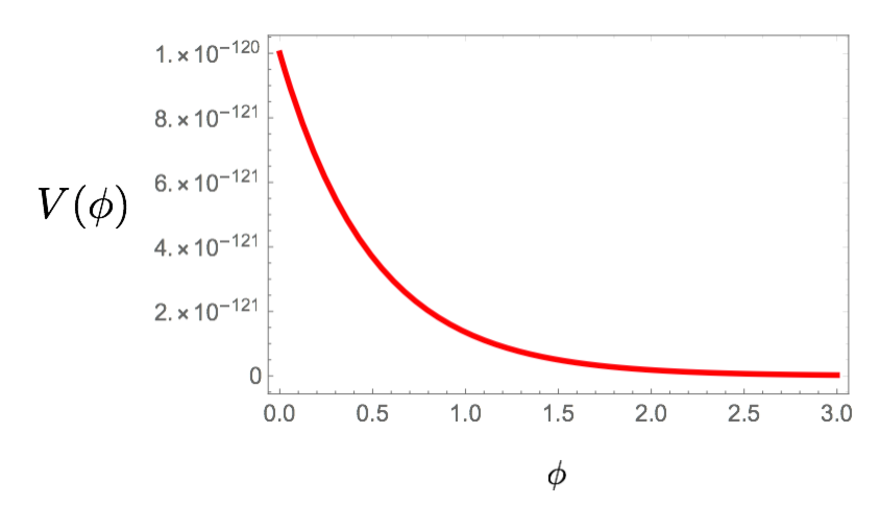
\includegraphics[width = 0.45\textwidth]{Sections/Figures/Runaway1.pdf} \qquad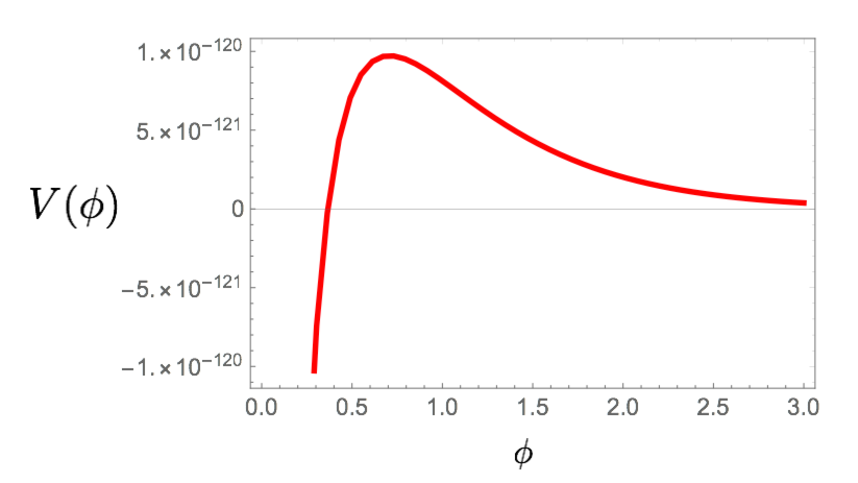
\includegraphics[width = 0.4\textwidth]{Sections/Figures/Runaway2.pdf}
\caption{Typical runaway potentials: the scalar potentials derived from eq. (\ref{E:DSrunaway}) for $p=3$ (left-hand side) and $p=1$ (right-hand side).}
\label{F:runaways}
\end{figure}

In fact, it has been shown using $N=1$ supergravity that all the typical string moduli -- whether bulk or local, whether lifted by perturbative or non-perturbative superpotentials -- have potentials that satisfy either $\epsilon_V > 1$ or $\rho_V < 0$ and so cannot drive an accelerated expansion, see Tab. \ref{quintrunnogos} \cite{Bento:2020fxj}. These results have been extended in \cite{Cicoli:2021fsd} considering no-scale models in type IIB, IIA and heterotic string compactifications. The limitations from string-inspired 4-dimensional $N=1$ supergravity on obtaining slow-roll potentials are reminiscent of similar results from \cite{Hellerman:2001yi} which show that, for a class of supersymmetric theories, it is impossible to relax into an asymptotic zero-energy supersymmetric minimum whilst accelerating (see also \cite{Rudelius:2021azq}). The theories considered are those with a single field with exponential potential $V\sim e^{-c\phi/M_{\rm Pl}}$; indeed, if the potential is to have a zero-energy supersymmetric vacuum and support $w_{\rm DE}={\rm constant}$ quintessence-like evolution, then it must have this form asymptotically, with $|c|< \sqrt{2}$. Assuming that the dynamics is indeed towards a zero-energy supersymmetric minimum at $\phi \rightarrow \infty$, Ref. \cite{Hellerman:2001yi} shows how 4-dimensional $N=1$ supersymmetry implies that having $V>0$ requires $c > \sqrt{6}$ and thus excludes slow-roll.   


\begin{table}[ht]
\begin{center}
\centering
\begin{tabular}{| c | c | c | c | c |}
\hline
{\cellcolor[gray]{0.9}$K$} & {\cellcolor[gray]{0.9}$W$} & {\cellcolor[gray]{0.9}$V>0 \quad \epsilon_V<1$} \\
\hline
\hline
$-p\ln(\Phi+\bar{\Phi})$ & $W_0 + A\,e^{-a\Phi}$ & no-go \\
\hline
$-p\ln(\Phi+\bar{\Phi})$ & $W_0 + A\,\Phi^n$ & no-go \\
\hline
$k_0 + \frac{|\Phi|^{2p}}{k_1}$ & $W_0 + A\,e^{-a\Phi}$  & no-go \\
\hline
$k_0 + \frac{|\Phi|^{2p}}{k_1}$ & $W_0 + A\,\Phi^n$ & no-go except for $p=n$ \\
\hline
$k_0 + \frac{(\Phi+\bar{\Phi})^{2p}}{k_1}$ & $W_0 + A\,e^{-a\Phi}$  & no-go \\
\hline
$k_0 + \frac{(\Phi+\bar{\Phi})^{2p}}{k_1}$ & $W_0 + A\,\Phi^n$ & no-go except for $p=n$ \\
\hline
\end{tabular}
\end{center} 
\caption{Summary of no-go theorems for string inspired supergravity models of single-field runaway quintessence, and parameter points that evade them. The K\"ahler potentials correspond, respectively, to bulk moduli, fibre moduli and blow-up moduli, and the superpotentials correspond to the flat direction $\Phi$ being lifted, respectively, by a leading non-perturbative effect or a leading perturbative one.  No-scale scenarios, having $K=-3\ln(\Phi + \bar{\Phi})$ and $W$ independent of $\Phi$, are included in the case that no-scale-breaking occurs via non-perturbative corrections to $W$.}  
\label{quintrunnogos}
\end{table}  

Note that we have -- as is usual in quintessence and as is entirely unsatisfactory in string theory -- left aside the cosmological constant problem and the fact that supersymmetry in the Standard Model sector must be broken at least at TeV scales which is clearly a challenge for supersymmetric vacua where the supersymmetry breaking scale would naturally be set by the dark energy scale.  At the same time, the difficulties in obtaining runaway directions that sustain accelerated expansion seem to extend to non-supersymmetric setups. The runaway potentials 
associated with NS-NS tadpoles in non-supersymmetric string theories are also too steep for quintessence, taking the form $V=\Lambda\, e^{-\gamma \phi}$ with $\gamma=\frac52, \frac32, \frac32$ in the Einstein frame, for the SO(16)$\times$SO(16) theory, the orientifold $USp(32)$ Sugimoto model, and the type 0B' model, respectively (see \cite{Basile:2020mpt} for an extension of dS no-go theorems to non-supersymmetric string theories).

These no-go theorems against single-field runaway quintessence support the conjecture against dS vacua, which are indeed best motivated at the asymptotic boundary of moduli space \cite{Ooguri:2018wrx}. However, as we will discuss in Sec. \ref{S:multiq}, there may be paths to 
evade these no-go results by considering multifield scenarios.

\subsubsection{Hilltop quintessence}

Alongside runaway moduli, which are ubiquitous in string compactifications, dS maxima are also very easy to find. For example, the Dine-Seiberg runaway potential in eq. (\ref{E:DSrunaway}) for $p=1$ is shown in Fig. \ref{F:runaways} to have a dS hilltop. In \cite{Olguin-Tejo:2018pfq}, the possibility of sourcing quintessence at the hilltop was explored (see \cite{Dutta:2008qn} for a phenomenological analysis of hilltop quintessence). If the modulus starts close to the hilltop, it can remain frozen there by Hubble friction for much of the cosmological history, first sourcing an effective cosmological constant and then turning into a rolling quintessence field with observable consequences. The parameters could be chosen to match the observed dark energy, consistent with the refined dS swampland conjecture (see Secs.~\ref{S:DEswamp} and \ref{Sec:Swamp} below) and with sub-Planckian field displacements. Quantum fluctuations $\Delta \varphi \sim H/(2\pi)$ leave the field within the viable window close to the hilltop until $H \sim 0.01\,M_{\rm Pl}$. Although there is no need for fine-tuning in the Lagrangian parameters, the fine-tuning of initial conditions is difficult to motivate, perhaps resorting to some anthropic danger in starting from a point in field space that leads into a steep runaway.

Of course this is just a scenario, and even if motivation for the initial conditions could be found, work would need to be done to embed it in a fully fledged string construction with moduli stabilisation and control over subleading corrections; in particular it may be a challenge to achieve sufficient sequestering to hide fifth forces, higher order instanton corrections may not be suppressed, and -- as is usual in quintessence scenarios -- the cosmological constant problem and vacuum contributions from the susy-breaking visible sector have not been addressed. Further attention to the hilltop scenario was given in \cite{Cicoli:2021skd}, using the dS maximum for the volume modulus in the KKLT scenario, where it was found that matching with the observed dark energy would require an unacceptably light gravitino and light volume modulus.


\subsubsection{Axions as quintessence}

Axions are arguably the most attractive quintessence candidates \cite{Kaloper:2008qs, Panda:2010uq, Choi:1999xn,Cicoli:2021skd} as ($i$) being pseudo-scalars they evade the most stringent spin-independent fifth force bounds; ($ii$) they enjoy approximate shift symmetries which restrict the allowed couplings and protect the axion mass and potential energy density, which are otherwise UV sensitive quantities; ($iii$) their potential is generated by exponentially suppressed non-perturbative effects which can naturally reproduce the required hierarchy between the dark energy potential and the potential which fixes the volume modulus at leading order (for example via perturbative effects which break supersymmetry spontaneously) guaranteeing $M_{\rm soft}\gtrsim 1$ TeV and $m_{\mathcal{V}}\gtrsim 1$ meV in a way compatible with $m_q \sim 10^{-32}$ eV. 

From the string theory point of view, a rather generic prediction is the existence of a 
large number of axions \cite{Green:1987mn, Banks:1996ea, Banks:2002sd, Svrcek:2006yi, Conlon:2006tq}  -- sometimes called an \emph{axiverse} \cite{Arvanitaki:2009fg} -- arising from the KK reduction of higher-dimensional form fields on the topological cycles of the compactification space. As an internal space can easily have $\mathcal{O}(100)$ distinct cycles, there can be $\mathcal{O}(100)$ axions. Typically, the axion directions will be perturbatively flat due to shift symmetries descending from higher-dimensional gauge symmetries, and which may subsequently be lifted by non-perturbative effects that give masses $\sim \mathcal{O}(e^{-\tau}M_{\rm Pl})$ with $\tau$ the partner saxion that measures the size of the corresponding cycle. 

In principle, the range of axion masses present can cover a wide region all the way down to quintessence-like masses $H_0 \sim 10^{-33}$ eV and beyond, which could include dark energy candidates as well as possible ultra-light axion dark matter with $m \sim 10^{-22}$ eV \cite{Hui:2016ltb, Cicoli:2021gss}. However, note that this would require the presence of many non-perturbative effects in the compactification, all with different origins and of different magnitudes, with the corresponding saxions fixed at higher masses (to avoid cosmological problems). See \cite{Marsh:2015xka} for a review on axion cosmology and \cite{Krippendorf:2018tei} for a discussion on possible macroscopic compact objects from ultralight string axions. For an analysis studying the coupled evolution with dark matter see \cite{Kumar:2013oda}.

One specific realisation of this idea can be found in the LVS scenario \cite{Cicoli:2021skd}. At leading order and considering an appropriate uplifting sector, $\mathcal{V}$ is fixed by $\mathcal{O}(\alpha'^3)$ effects in a Minkowski vacuum where supersymmetry is spontaneously broken. At this level of approximation, the axionic partner of the volume modulus is a flat direction due to its shift symmetry that is perturbatively exact. Hence the mass scale of $\mathcal{V}$ and the supersymmetry breaking scale can be safely decoupled from $H_0$. The volume axion is lifted by tiny non-perturbative corrections that are exponentially suppressed in a power of the exponentially large volume, and so can naturally reproduce the dark energy scale since 
\begin{equation}
\setlength\fboxsep{0.25cm}
\setlength\fboxrule{0.4pt}
\boxed{
V_{\rm DE} \simeq e^{-\sqrt{\frac32} \frac{M_{\rm Pl}}{f}}\,M_{\rm Pl}^4\left[1-\cos\left(\frac{\varphi}{f}\right)\right]\,,
}
\label{Vax}
\end{equation}
where $\varphi$ is the canonically normalised volume axion with decay constant:
\begin{equation}
f = \sqrt{\frac32}\frac{N\,M_{\rm Pl}}{2\pi\mathcal{V}^{2/3}} \,   
\end{equation}
where $N=1$ for a Euclidean D3-brane instanton while $N$ is the rank of the condensing gauge group for gaugino condensation on D7-branes. Reproducing $V_{\rm DE}\sim 10^{-120}\,M_{\rm Pl}^4$ from (\ref{Vax}) requires $M_{\rm Pl}/f\sim 300$, and so moderately large volumes, $\mathcal{V} \sim 10^3 - 10^4$, which are however still large enough to trust the effective field theory. Moreover $M_s\sim 10^{16}$ GeV, $m_{3/2}\sim 10^{14}$ GeV and $m_{\mathcal{V}}\sim 10^{12}$ GeV, together with $m_q \sim 10^{-32}$ eV. 

Let us stress that any axionic field whose saxion partner is stabilised by perturbative effects will have such doubly exponentially suppressed masses. For example, whereas blow-up moduli tend to be stabilised as for their axionic partners non-perturbatively, leading to masses for saxions and axions of the same order, the saxions associated with fibre moduli tend to be stabilised perturbatively, and thus end up being heavier than their axion partners, allowing for an EFT where the saxions can be integrated out to leave an ultra-light axions to drive quintessence (see \cite{Emelin:2018igk} for a discussion on how, otherwise, lifting axion away from its minimum can lead to a steep runaway instability in the saxion direction).  

Unfortunately, as we have already discussed, it is not sufficient to have a light scalar field to drive a period of accelerated expansion; the scalar potential must be sufficiently flat. This is not the case for the potential (\ref{Vax}) since the axion decay constant is sub-Planckian, $f\sim M_{\rm Pl}/300$, while a sufficiently shallow potential would require a super-Planckian field displacement and axion decay constant \cite{Freese:1990rb}. Note that this is not just a consequence of matching the correct dark energy scale, but also a condition to trust the effective field theory. In fact, axion decay constants typically scale as $f \sim M_{\rm Pl}/\tau$ \cite{Svrcek:2006hf, Svrcek:2006yi, Arvanitaki:2009fg, Cicoli:2012sz}. Hence $\tau \gtrsim 1$ implies that axion decay constants are always sub-Planckian. Indeed super-Planckian decay constants are very difficult to obtain within string theory, and recent discussions in the context of the string swampland even suggest that they may be forbidden in quantum gravity via axionic versions of the weak gravity conjecture \cite{Klaewer:2016kiy, Blumenhagen:2017cxt, Palti:2017elp, Cicoli:2018tcq, Cicoli:2021gss}.

However, there are other possibilities for axions to drive an accelerated expansion without a super-Planckian decay constant: 
\begin{itemize}
\item \textbf{Axion hilltop quintessence:} for a single axion field, by fine-tuning the initial conditions sufficiently close to its hilltop, an accelerated expansion can be achieved \cite{Kamionkowski:2014zda, Cicoli:2021skd}. Even if one might think that not much tuning is necessary to achieve less than $1$ e-folding of late-time accelerated expansion, the initial conditions that allow for quintessence are likely to be destroyed by inflation. In fact, during inflation the axion is an ultra-light field which acquires quantum fluctuations of order $\Delta\varphi\sim H_{\rm inf}/(2\pi)$. The initial vicinity to the maximum is determined by the value of the axion decay constant. For example, for $f\sim 0.02\,M_{\rm Pl}$ which is roughly the largest possible value of $f$ compatible with a large volume expansion, this distance in Planck units has to be smaller than $10^{-18}$ \cite{Cicoli:2021skd}, imposing $H_{\rm inf}\lesssim 10^{-18}\,M_{\rm Pl}\sim 1$ GeV. For smaller values of $f$, the tuning gets even worse.

\item \textbf{Axion alignment quintessence:} for two or more light axionic fields, an alignment mechanism \cite{Kim:2004rp, Dimopoulos:2005ac, Shiu:2015xda, Cicoli:2014sva} may generate an effective super-Planckian decay constant out of two or more sub-Planckian decay constants (see \cite{Cicoli:2018kdo} for other possibilities for axion quintessence, which rely on the presence of a dS minimum). The lightest axion could play the role of dark energy while the axion which remains heavy could potentially account for dark matter.
\end{itemize}

\subsubsection{Branes, extra dimensions and string symmetries}
\label{S:DEbranes}

As a key constraint on quintessence candidates is always their interactions with Standard Model matter resulting in fifth forces, a natural place to look for string theory quintessence candidates is from hidden sector D-branes, as they may be coupled to visible sector D-branes with weaker-than-Planckian couplings.  

\paragraph{k-essence from branes}

Refs. \cite{Martin:2008xw, Gumjudpai:2009uy} explored whether the DBI action could give rise to quintessence attractor tracker solutions for the scalar field representing the position of the brane. This starts with a string-inspired, phenomenological action:
\begin{equation}
\setlength\fboxsep{0.25cm}
\setlength\fboxrule{0.4pt}
\boxed{
S_{\rm DBI}= -\int d^4x \; a^3(t) \left(T(\phi)W(\phi)\sqrt{1-\frac{\dot{\phi}^2}{T(\phi)}}-T(\phi)-\tilde{V}(\phi)\right), \label{E:DBIessence}
}
\end{equation}
where $T(\phi)$ is the warped tension of the brane and $W(\phi)$ and $\tilde{V}(\phi)$ are potential terms, the first coming from the nature of the D-brane stack (e.g. supersymmetry breaking effects, non-Abelian sectors, worldvolume fluxes) and the second from possible interactions with the bulk and other brane stacks.  This gives rise to an equation of state:
\begin{equation}
w_\phi = \frac{T(\phi)(\gamma-W(\phi))-\gamma \tilde{V}(\phi)}{\gamma T(\phi)(\gamma W(\phi)-1)+\gamma\tilde{V}(\phi)}
\end{equation}
with $\gamma = \left( 1-\frac{\dot{\phi}^2}{T(\phi)}\right)^{-\frac12}$. The simplest case is of a D3-brane moving in a 5-dimensional AdS space, describing the mid-region of a warped throat, $T(\phi) \propto \phi^4$ and $W(\phi)=1$. Assuming moreover that $\tilde{V}(\phi) \propto T(\phi)$ is justified as it follows from $\gamma=\,$constant, which in turn is an attractor scaling solution. Then $w_\phi=2w+1>1$, with $w$ the equation of state of the background fluid, so that $\phi$ scales faster than the background fluid and can never come to dominate the universe \cite{Martin:2008xw}.  More general forms for the functions characterising the DBI action, which may or may not derive from string theory, allows for viable k-essence models \cite{Gumjudpai:2009uy}, but only for super-Planckian field excursions.  Also, although  small scales for the vacuum energy and quintessence mass can be arranged, their robustness against quantum corrections is not yet addressed, 

\paragraph{Fine-tuning, branes and supersymmetry breaking}

Branes and extra dimensions potentially allow for symmetries which can help address the fine-tuning problems in dark energy in non-trivial ways. For example, supersymmetry may be badly broken in the visible sector branes, say around TeV scale, thus explaining the absence of superpartners for the Standard Model, whilst the large localised vacuum energy may curve the extra dimensions rather than the branes themselves.  Meanwhile, supersymmetry breaking in the bulk could be suppressed with respect to the visible sector branes by the Planck scale, leading to a corresponding suppression in the final vacuum energy. 

This idea was explored in the Supersymmetric Large Extra Dimensions (SLED) scenario \cite{Aghababaie:2003wz, Burgess:2004ib}, where two large extra dimensions explain the hierarchy problem \cite{Arkani-Hamed:1998jmv, Antoniadis:1998ig} and bring the string scale down to around TeV, whilst the KK scale and gravitino mass are suppressed to around meV such that bulk contributions to the vacuum energy go as $M_{\rm KK}^2 m_{3/2}^2 \sim {\rm meV}^4$. An interesting stringy embedding of the SLED scenario with anisotropic moduli stabilisation that leads to $2$ extra dimensions much larger than the other $4$ has been presented in \cite{Cicoli:2011yy}. In SLED, dark energy emerged as a quintessence scenario using the volume modulus associated with the large extra dimensions, which develops a logarithmic slow-roll potential \cite{Albrecht:2001cp, Albrecht:2001xt}.  

A related scenario based on \cite{Cicoli:2011yy} is \cite{Cicoli:2012tz}, which considers large extra dimensions in the context of LVS. Here, the quintessence field is a fibre modulus which has weaker-than-Planckian couplings to a visible sector that is localised on a blow-up modulus having no intersection with the quintessence fibre. As already mentioned, having a quintessence sector which is geometrically separated from the visible sector helps in suppressing dangerous fifth forces and time-variation of coupling constants. The dark energy potential is generated by tiny poly-instanton corrections to the superpotential and the model shares several features with those of a typical SLED model: $2$ exponentially large extra dimensions, a gravitino mass of order the cosmological constant scale and TeV-scale gravity.

For these proposals to really work, it is necessary to control the loops on the branes, where supersymmetry is only non-linearly realised; their contributions to the vacuum energy would need to be absorbed by backreaction onto the extra dimensional curvature, but they may instead lead to high curvature on the brane or instabilities and runaway solutions.  

Progress on these questions may be facilitated by recently developed tools in coupling non-supersymmetric matter to supergravity \cite{Komargodski:2009rz, Bergshoeff:2015tra, Dudas:2015eha, DallAgata:2015zxp, Schillo:2015ssx, Parameswaran:2020ukp}. This has been initiated in \cite{Burgess:2021juk}, where evidence was found that the supergravity form of the action -- and a small splitting in the gravity supermultiplet --  is stable against integrating out heavy, non-supersymmetric particles, thanks to the interplay with auxiliary fields associated with gravity, the goldstino and other supermultiplets in the supersymmetric gravity sector.  Having a gravity sector that is supersymmetric down to low energies, coupled to a visible sector where supersymmetry is non-linearly realised, is also motivated by the fact that gravity would have the weakest couplings to any supersymmetry breaking sector \cite{Arkani-Hamed:2006emk}. Cosmological bounds on the light gravitini and moduli that would arise with enhanced supersymmetry in the gravity sector are discussed in \cite{Kawasaki:2008qe, Feng:2010gw, Coughlan:1983ci, Banks:1993en, deCarlos:1993wie, Conlon:2007gk}.

How supersymmetry may help in the UV stability of dark energy models such as quintessence has been pursued further in the scenario of `yoga dark energy' \cite{Burgess:2021obw}. This proposes that a very supersymmetric gravity sector, combined with an accidental approximate scale invariance  and a `relaxon' scalar field \cite{Graham:2019bfu} with $m \lesssim m_e$ that dynamically reduces the leading non-gravitational vacuum energy, might explain the cosmological constant problem and the observed dark energy.  The supersymmetric gravity sector could be realised by brane supersymmetry breaking \cite{Sugimoto:1999tx, Dudas:2000nv, Antoniadis:1999xk, Kallosh:2014wsa, Kallosh:2016aep, GarciadelMoral:2017vnz, Cribiori:2019hod}, whilst accidental approximate scale invariance is a generic property of low-energy string vacua \cite{Berg:2005ja, Cicoli:2007xp, Cicoli:2021rub} and its interplay with supersymmetry is studied in \cite{Burgess:2020qsc}. The string interpretation of the relaxon remains to be explored in detail, as well as how well the scenario stands up to naturalness and phenomenological conditions.  

Interestingly, the UV completion \cite{Cribiori:2020sct} of brane supersymmetry breaking is not the standard supersymmetry but rather a so-called misaligned supersymmetry \cite{Dienes:1994np, Cribiori:2021txm}. The possibility that string theoretic modular invariance and misaligned symmetry may help with the cosmological constant problem has been discussed in \cite{Dienes:2001se}.  Although no complete realisation of this idea has been found, there exists non-supersymmetric setups that have an exponentially suppressed vacuum energy to two-loops \cite{Kachru:1998hd, Kachru:1998pg, Abel:2015oxa, Abel:2017rch}, thanks to Bose-Fermi cancellations between the massless field degeneracies in a non-supersymmetric visible sector and a non-supersymmetric hidden sector.


\subsubsection{Dark energy and the swampland}
\label{S:DEswamp}

The swampland aims to map out the set of effective field theories that can be ultraviolet completed consistently with quantum gravity (see Sec.~\ref{Sec:Swamp} below). The dS swampland conjecture \cite{Obied:2018sgi, Garg:2018reu, Ooguri:2018wrx} proposes that the scalar potential in any consistent effective field theory must satisfy either $|\nabla V| \gtrsim \frac{c}{M_{\rm Pl}}V$ or $\textrm{min}(\nabla_i \nabla_j V)\lesssim -\frac{c'^2}{M_{\rm Pl}^2} V$ where $c,c'>0$ are $\mathcal{O}(1)$ universal constants, ruling out even metastable dS vacua. Support for the dS conjecture is found in the parametrically asymptotically controlled regime of string theory via the swampland distance conjecture and Bousso's covariant entropy bound \cite{Ooguri:2018wrx} (it is important to note that the candidate string dS vacua discussed in Sec. 3 rely on numerical control rather than parametric control; see also \cite{Dvali:2018jhn, Dvali:2018fqu} for other quantum gravity arguments against long-lived dS and \cite{Rudelius:2019cfh} for some motivation via the problems of eternal inflation). In this regime, the strong dS conjecture \cite{Rudelius:2021azq} states that the strong energy condition should be satisfied at late times, implying $c=\sqrt{2}$, which would also forbid asymptotic accelerated expansion. 

A solution to the dark energy problem seems therefore to lie in a region of moduli space without full parametric control over the effective field theory, i.e.~where one cannot make approximations arbitrarily good. dS vacua or quintessence solutions could however be obtained with numerical control thanks to underlying parameters, like $W_0\ll 1$ in KKLT or $\mathcal{V}^{-1}\sim e^{-1/g_s}\ll 1$ in LVS, which can be made very small, even if not arbitrarily small (since the number of moduli and the D3 tadpole set a lower bound on $W_0$ and $g_s$). Note moreover that quintessence model building features the same challenges as the construction of dS vacua with however additional constraints coming from fifth forces, radiative stability of the quintessence mass, and huge hierarchies in the moduli stabilising scalar potential \cite{Cicoli:2021skd}. Hence, from this perspective, quintessence, instead of looking like a viable alternative to dS, seems to be under even less control than dS vacua. This consideration raises therefore some doubts on the validity of the dS conjecture in regions of the moduli space with numerical, instead of parametric, control due to the observational evidence of a present epoch of accelerated expansion and the current lack of robust dark energy alternatives to dS and quintessence.

Allowing for effective field theories with quintessence-like configurations, the trans-Planckian censorship conjecture \cite{Bedroya:2019snp} proposes that the possibility of sub-Planckian scale fluctuations redshifting until they cross the horizon and classically freeze out is unphysical, and therefore any epoch of super-luminal expansion must have a finite lifetime $\Gamma < H \ln H$. In asymptotic regions of field space, the trans-Planckian censorship conjecture implies the dS swampland conjecture with $c = \sqrt{2/3}$, however, deep in the interior of field space the former is compatible with metastable dS so long as it is sufficiently unstable quantum mechanically.

Ref. \cite{Agrawal:2018own} considered the implications of the swampland dS conjecture and the swampland distance conjecture and concluded that they would be in tension with early universe cosmic inflation: CMB observations bound the single-field inflationary slow-roll parameter $\epsilon < 0.0044$, which in turn bound the order one constant in the dS conjecture $c<0.094$. Moreover, any future detection of a tensor-to-scalar ratio of order $r \sim 0.01$ would indicate an inflaton field excursion of $\Delta \phi \sim 2\,M_{\rm Pl}$. 
%IZ: Adding Shi  1809.05507
In \cite{Han:2018yrk}  the authors coupled the vanilla exponential quintessence potential to the Higgs sector, and found that this coupling helps in addressing the electroweak vacuum instability problem. Moreover, they obtained the bound  $c>0.35$, consistent with current constraints $c\lesssim 0.6$ \cite{Agrawal:2018own,Akrami:2018ylq,Heisenberg:2018yae}.


Whether or not the swampland conjectures turn out to be true, it is interesting to consider to what new ideas they may lead. Ref. \cite{Montero:2022prj} uses the distance/duality conjecture, the smallness of dark energy, and current (albeit rather model dependent) observational constraints on extra dimensions \cite{Workman:2022ynf, Hannestad:2003yd}, to argue that the universe is in an asymptotic region of field space with a single large extra dimension -- named the `dark dimension' -- of size $l \sim \mu m \sim ({\rm meV})^{-1}$ along with a fundamental gravity scale $M \sim 10^{10}$ GeV. Whereas the brane scenarios discussed in Sec. \ref{S:DEbranes} use large extra dimensions to bring fundamental gravity down to the TeV-scale and to lower the supersymmetry breaking scale in the gravity sector, here the large extra dimension is motivated by the expectation that the one-loop vacuum energy goes as $M_{\rm KK}^4\sim ({\rm meV})^4$ for a tower of light states starting at $M_{\rm KK}$. It goes without saying that finding a viable string embedding with moduli stabilisation of the large dark dimension scenario is a difficult task. Moreover, it remains an open question how an accelerated cosmology is obtained in the asymptotic region of field space. 

Nevertheless, if dark energy is sourced by a rolling scalar field, the asymptotically exponentially light tower of states implied by the swampland distance conjecture could play the role of dark matter which continuously becomes lighter as the dark energy field rolls down its potential  \cite{Agrawal:2019dlm}. This so-called `fading dark matter' scenario may help to address the tensions in the late-time measurements of $H_0$ and $\sigma_8$ compared to the values inferred from early-times using the $\Lambda$CDM model. Alternatively, the tower of states may correspond to the massive KK gravitons, universally coupled to the Standard Model and produced as dark matter as the Standard Model sector cools down \cite{Gonzalo:2022jac}. Ref. \cite{Anchordoqui:2022txe} observes that a mesoscopic large extra dimension slows down the rate of Hawking radiation for black holes, thus prolonging the survival of low-mass primordial black holes, which can then compose all of dark matter. The correspondence between a 5-dimensional primordial black hole and 5-dimensional massive KK modes interpretation of dark matter was discussed in \cite{Anchordoqui:2022tgp}. 


\subsubsection{Multi-field quintessence} 
\label{S:multiq}

Multi-field quintessence models can help overcome several of the problems suffered by single-field models, and are also well-motivated by string theory given the large numbers of scalar fields that arise in string compactifications, with non-trivial target-space geometries. Similarly to hybrid inflation, multi-field models provide mechanisms to exit the accelerated expansion. They also provide new avenues to achieve accelerated expansions with steep potentials, via non-geodesic trajectories or gradient flows. And sufficiently shallow potentials may be found in regions of weak couplings and parametric control, where competing terms in the multifield asymptotic limit can allow for geodesic trajectories along gradient flows, which represent shallow valleys in the multi-dimensional moduli space. We will now discuss these various proposals in more detail.

\paragraph{Hybrid quintessence for a graceful exit:}

The conceptual problems presented by an eternal dS, e.g. the absence of a well-defined S-matrix, are shared by quintessence models \cite{Hellerman:2001yi, Fischler:2001yj} unless there is a mechanism to end quintessence at some time in the future. Similarly to hybrid inflation \cite{Linde:1993cn}, this can be achieved in a multi-field hybrid quintessence model. A stringy realisation of this idea is given by quintessence from $2$ D3-branes separated by some large distance, $r$, and at some relative angle, $\theta$ \cite{Halyo:2001fb}. The relative angle breaks supersymmetry and generates a tracker quintessence potential for the $2$ fields: $V(\phi,\theta) = \theta^2 \frac{M_s^8}{M_{\rm Pl}^2 \phi^4}$. To obtain the observed dark energy scale, $\rho \sim 10^{-120}M_{\rm Pl}^4$, with $\theta, \phi \sim M_{\rm Pl}$, requires $M_s \sim$ TeV and hence $2$ large extra dimensions.  In the early universe, domination by radiation or matter ensures that $H>m_\theta$, so that $\theta$ is frozen at a constant VEV $\mathcal{O}(M_{\rm Pl})$.  If $\rho_\phi$ is greater than the energy density of the tracker solution, $\phi$ rolls quickly down its potential until it freezes at some VEV $\mathcal{O}(M_{\rm Pl})$, due to the large redshift of kinetic energy, by which time $\rho_\phi$ is much less than the tracker energy density. At this point both $\theta$ and $\phi$ behave as frozen quintessence with $w\approx -1$, and eventually the quintessence comes to dominate the universe. Later, $H$ falls below $m_\theta$, $\theta$ begins to roll, the accelerated expansion ceases, and the potential eventually vanishes as $\theta$ settles at its minimum, yielding to another era of matter domination. Although this scenario solves the problem of a well-defined S-matrix, it requires super-Planckian field displacements to achieve a shallow enough potential to drive the accelerated expansion as well as a moduli stabilisation scenario that results in two large extra dimensions.

\paragraph{Non-geodesic trajectories in string constructions:}

Just as for inflation, having multiple fields provides new avenues to achieve accelerated expansion with steep potentials via curved non-geodesic trajectories in the multi-dimensional target-space. String compactifications do give rise to non-linear sigma models in their 4-dimensional $N=1$ supergravity descriptions, providing in principle interesting target-space geometries for non-geodesic behaviour.\footnote{However, as shown in \cite{Aragam:2021scu}, non-geodesic trajectories in supergravity seem to require very large field space curvatures.} Moreover, non-geodesic trajectories can be longer than the geodesic distances that determine the masses of towers of states \cite{Landete:2018kqf, Hebecker:2017lxm}. 

Various effective field theory multi-field models have been proposed that are consistent with observational data and the swampland conjectures \cite{Sonner:2006yn, vandeBruck:2009gp,  Brown:2017osf, Russo:2018akp, Achucarro:2018vey, Cicoli:2020cfj, Cicoli:2020noz, Akrami:2020zfz}. Ref. \cite{Brinkmann:2022oxy} considers instead string-inspired multi-field models composed of saxion-axion pairs with the kinetic couplings and scalar potential expected for either closed string universal moduli or non-universal moduli such as blow-up modes. A possible setting for the universal moduli is \cite{Saltman:2004sn, Gallego:2017dvd}; these involve type IIB flux compactifications with all the complex structure moduli and axio-dilaton stabilised, leaving a single K\"ahler modulus with $K=-p\ln(T+\bar{T})$ and $V=V_0/(T+\bar{T})^p$ and $p=3$. Other string settings corresponding to different values of $p$ are outlined in Tab. \ref{T:multiunimodq}. A possible setting to consider candidate blow-up modes is type IIB orientifold flux compactifications with internal Calabi-Yau of the `weak Swiss cheese' form \cite{Cicoli:2018tcq}, assuming just one universal modulus, $\tau_b$, and one blow-up mode, $\tau_s$, with $\tau_s \ll \tau_b$, for which $K=-2\ln{\mathcal{V}} = -3\ln \tau_b + 2 \left(\tau_s/\tau_b\right)^{3/2}$. 

This yields specific polynomial kinetic couplings and scalar potential.  For the string-motivated couplings and potential discussed, and assuming that the dark energy epoch is entered from an epoch of matter domination as in our universe, Ref. \cite{Brinkmann:2022oxy} found that -- although multi-field accelerated cosmologies could easily be found -- none passed through the current observed values for $(\Omega_{\rm DE}, w_{\rm DE})\approx(0.7,-1)$ (starting from these observed values and working backwards, it was found that the observed values could be reached via initial conditions of kinetic domination). It remains an open question whether observationally viable models could be found in other multi-field string setups, with different couplings and potentials and/or more than two fields.  

\begin{table}[htp]
\begin{center}
\begin{tabular}{l c c c c c }\hline
\cellcolor[gray]{0.9} $p$ & \cellcolor[gray]{0.9} $X$ & \cellcolor[gray]{0.9} Theory & \cellcolor[gray]{0.9} Sources &   \cellcolor[gray]{0.9} $\mathcal{M}_{\rm internal}$ & \cellcolor[gray]{0.9} References \\ [5pt]
\hline
$1$ & $S = e^{-\varphi} + {\rm i}\, a$ & Heterotic & --- & $\mathrm{SU}(3)$ str. & \cite{Font:1990nt} 
\\ [5pt]
$2$ & $T_2 = {\rm Vol}(\Sigma_4^{(2)}) + {\rm i} \int_{\Sigma_4^{(2)}} C_{(4)}$ & Type IIB & D3/D7, O3/O7 & K3-fibered $\mathrm{CY}_3$  & \cite{Cicoli:2011it,Cicoli:2016xae,Cicoli:2017axo} 
\\[5pt]
$3$ & $T = {\rm Vol}(\Sigma_4) + {\rm i} \int_{\Sigma_4} C_{(4)}$ & Type IIB & D3/O3 & $\mathrm{CY}_3$  & \cite{Saltman:2004sn} 
\\[5pt]
$7$ & $Z = {\rm Vol}(\Sigma_3) +{\rm i}\int_{\Sigma_3} A_{(3)}$ & M-theory & KK6/KKO6 & $\mathrm{G}_2$ str. & \cite{Blaback:2019zig}
\\[5pt]
\bottomrule
\end{tabular}
\end{center}
\caption{Examples of string constructions having a 4-dimensional saxion-axion system with $K=-p\ln(\Phi+\bar{\Phi})$ and $V=e^K V_0$, which yields an exponential kinetic coupling and exponential runaway potential in the canonically normalised saxion. The two-field models arise after all other moduli present in the given setup are fixed. Table from \cite{Brinkmann:2022oxy}.}
\label{T:multiunimodq}
\end{table}

\paragraph{Gradient flows in string constructions:}

Ref.~\cite{Calderon-Infante:2022nxb} shows that the no-go theorems for single-field runaway quintessence in 4-dimensional $N=1$ supergravity can be evaded by considering saxionic multi-field models. Again focusing on regions of the moduli space at infinite field distance, which give parametric control as the weak coupling parameter in the relevant perturbative expansion goes to zero in that limit, the multi-field trajectories found turn out to be geodesic ones.  Asymptotically, the trajectories are gradient flows, completely determined by the shape of the potential and the field space metric: these flows are parameterised by $\lambda$ with $\dot{\phi}^k(\lambda) = -\mathcal{F}(\lambda)\partial^k V(\lambda)$ where the smooth positive function $\mathcal{F}(\lambda)$ takes care of reparameterisation invariance. The important point is that, with multiple fields, different terms can compete with each other in the potential even in the asymptotic limit. Consider for example the 4-dimensional $N=1$ scalar potentials arising from F-theory compactified on a Calabi-Yau fourfold with $G_4$-flux. Assume also that the K\"ahler modulus, of which the superpotential is independent, allows for a no-scale cancellation leaving a positive-definite scalar potential $V_{\rm NS} = e^K K^{i\bar{\jmath}}D_i W \overline{D_j W}$. Then, the asymptotic limit when approaching an infinite distance singularity in complex structure moduli space, keeping the overall volume $\mathcal{V}$ constant and assuming that partner axions have been stabilised or remain as flat directions, takes the form:
\begin{equation}
V_{\rm NS} = \sum_{\bf{l} \in \mathcal{E}} A_{\bf{l}} \prod_{k=1}^n \left(\phi^k\right)^{l_k},
\end{equation}
for $n$ saxions $\phi^k$, $\mathcal{E} \subset \mathbb{Z}^n$ and $A_{\bf{l}} \in \mathbb{R}$. The powers $l_k$ are constrained and classified by the framework of asymptotic Hodge theory, and overall, coefficients are such that $V\geq 0$ asymptotically and $V\rightarrow 0$ along at least one trajectory towards infinity. Consider for simplicity Calabi-Yau fourfolds with $2$ complex structure moduli only. Now, for flux choices such that the asymptotic potential has a single dominant term, e.g. 
\begin{equation}
V_{\rm NS}=f_4^2\,\frac{1}{\phi^1\phi^2}
\end{equation}
with $\vec{\phi}(\lambda)=(\alpha \lambda^3, \lambda)$, the situation is similar to the single-field case and the potential is too steep to drive an accelerated expansion. However, there are also flux choices that allow more than one term to compete in the asymptotic limit, e.g. 
\begin{equation}
V_{\rm NS} = f_2^2 \,\frac{\phi^2}{\phi^1}+h_0^2\frac{\phi^1}{\left(\phi^2\right)^3},
\end{equation}
with $\vec{\phi}(\lambda)=\left(\frac{\sqrt{5}}{3}\vline\frac{f_2}{h_0}\vline \lambda^2, \lambda\right)$. It can be shown that the dS coefficient for such an asymptotic gradient flow is $\frac{|\nabla V_{\rm NS}|}{V_{\rm NS}} = \sqrt{\frac27}$, which is sufficiently small to allow for an accelerated expansion.  

It is important to note that the potentials just written have ignored the K\"ahler moduli, in particular the universal volume modulus. Unless the volume modulus is stabilised, it will also contribute to the dS coefficient, rendering the potential once again too steep for an accelerated expansion; at the same time, once the volume is stabilised, the no-scale cancellation, assumed in order to ensure a positive-definite scalar potential, needs to be revisited.  

\subsubsection{Coupled dark sector models} 

Another way to overcome difficulties in finding accelerating cosmologies in string theory are scenarios in which the dark energy and dark matter sectors are coupled. Although there are strong constraints on dark energy interacting with the visible sector, from solar-system and table-top tests of gravity, there are no such constraints on dark energy interacting with dark matter. Given the rich hidden sectors offered by string constructions, coupled dark sectors are well-motivated and also come with interesting phenomenological signatures (see \cite{Bolotin:2013jpa, Wang:2016lxa} for a review into phenomenological models of interacting dark energy/dark matter).  

\paragraph{DBI-essence with disformally coupled dark matter:}

One such scenario arises from D-branes, where, as in DBI quintessence, dark energy arises from open strings representing the radial position of a D-brane along a warped throat, and now dark matter arises from open strings representing matter on the same hidden sector brane \cite{Koivisto:2013fta}.  The action for the dark energy scalar takes the form (\ref{E:DBIessence}) with $T(\phi)=h^{-1}(\phi)$, the inverse warp factor, and $W(\phi)=1$. The action for the dark matter, originating at low energies from $N$ particles on the moving D3-brane, e.g. from vector fields which have acquired St\"uckelberg masses $m_i$, takes the form:
\begin{equation}
S_{\rm DM} = -\sum_{i=1}^N\int d^4x\, m_i \, \sqrt{-\bar{g}_{\mu\nu}\dot{x}_i^\mu \dot{x}_i^\nu}\delta^{(4)}(x_i(\tau)-x_i),
\end{equation}
where $\bar{g}_{\mu\nu}=h^{-1/2}g_{\mu\nu}+h^{1/2}\partial_\mu x^m \partial_\nu x^m g_{mn}$ is the pull-back of the 10-dimensional metric onto the brane, $x^M(\xi^\mu)$ are the embedding of the brane worldvolume into the spacetime, and we have chosen the static gauge $\xi^\mu=x^\mu$.  The energy density that follows from $S_{\rm DM}$ is:
\begin{equation}
\rho = \sum_{i=1}^N m_i \delta^{(4)}(x_i(\tau)-x_i)\left(\frac{1}{T_3 h(\phi)}\right)^\frac14\sqrt{\frac{\dot{x}^2}{g}}\left(1-h(\phi),(u^\mu\partial_\mu\phi)^2\right)^{-\frac12}
\end{equation}
with $u^\mu = \frac{\dot{x}_\mu}{\sqrt{-\dot{x}^2}}$, from which one obtains a (so-called `disformal' \cite{Bekenstein:1992pj}) coupling with the dark energy scalar, $\phi$.  This non-trivial coupling leads to a non-conservation of dark matter energy density and a non-standard time-evolution as the universe expands.  

Consider two concrete examples, namely ($i$) an AdS warp factor, $h(\phi) \sim \phi^{-4}$, corresponding to a D-brane in the mid-region of a Klebanov-Strassler throat together with a mass term for the scalar potential, $\tilde{V}(\phi) \sim \phi^2$ and ($ii$) a constant warp factor, $h(\phi)\sim$ constant, corresponding to a D-brane in the bulk or close to the tip of the throat, and an inverse power law potential, $\tilde{V}(\phi) \sim \phi^{-2}$. 

 In both cases, a dynamical systems analysis reveals a late-time accelerating scaling expansion, with the universe becoming asymptotically devoid of all matter whilst maintaining a constant rate of acceleration. The acceleration may ultimately end, however, depending on what happens when the dark D-brane eventually reaches the tip of the throat. Note that the usual slow-roll conditions and Hubble scale mass for the dark energy scalar, $\phi$, is not necessary for this acceleration, thanks to the non-canonical kinetic term in the DBI action. The observed dark energy scale is obtained for $m_\phi \sim 10^{-60} M_{\rm Pl}^2$, which can be achieved for a D-brane close the tip of the warp throat (although the cosmological constant problem, as usual, has not been addressed). The consequent interchanges between dark energy and dark matter suggests that their energy densities should be around the same order, providing a solution to the coincidence problem. As well as phenomenological questions on the implications of coupled dark sectors for structure formation, it also remains necessary to embed the interesting D-brane couplings and potential into a fully fledged string compactifications with stabilised moduli.

\paragraph{Dark matter assisted dark energy}

As well as explaining the coincidence problem, coupling dark energy to dark matter can help to achieve accelerated expansion in ways consistent with quantum gravity expectations; with a graceful exit from the dS epoch, thus allowing S-matrices to be consistently defined \cite{Gomez:2022}. 

Motivated by the prevalence of hidden sectors in string theory, the thermal dark energy scenario \cite{Hardy:2019apu} (cf. thermal inflation \cite{Lyth:1995ka}) proposes the existence of a light hidden sector that is still in internal thermal equilibrium in the present-day universe, thus constituting dark radiation. A light hidden scalar $\phi$ -- which can be a modulus or matter field -- can then be stabilised in a temperature-dependent metastable dS minimum, away from its true AdS or Minkowski minimum, thanks to its interactions with bosons $\chi^i$ and fermions $\psi^a$ in the thermal bath. For example, with interaction terms $\lambda_i \phi^2 \chi^i \chi^i$ and $y_a \phi \psi^a \bar{\psi}^a$, and hidden sector temperature $T_h$ much greater than the masses $m_{\chi^i}, m_{\psi^a}$ in the thermal bath, finite temperature effects contribute to the scalar potential for $\phi$ as:
\begin{equation}
V(\phi, T_h) = V(\phi,0) + b T_h^2 \phi^2\,,
\end{equation}
where the constant $b$ depends on the interaction couplings, $\lambda_i, y_a$.  Consider e.g. $\phi$ with a Higgs-like zero-temperature potential $V(\phi,0) = \lambda(\phi^2-\phi_0^2)^2$, with zero-temperature minimum at $\phi=\phi_0$ giving Minkowski space and $m_\phi=2\sqrt{\lambda}\phi_0$. Then, for sufficiently high hidden sector temperatures $T_h > T_c= \sqrt{\frac{2\lambda}{b}}\phi_0$, finite temperature effects stabilise $\phi$ at $\phi=0$, at a dS minimum with vacuum energy $\rho_{\rm DE}=\lambda \phi_0^4$. Phenomenologically viable regions of parameter space can be found for scalar masses $\lesssim \mu$eV, which are much larger than usual quintessence scales.  The metastable dS survives until hidden sector temperatures fall below $T_c$, around which time there will typically be a first-order phase transition to the true global Minkowski minimum, thus allowing a well-defined S-matrix.

A related scenario is `locked dark energy' \cite{Axenides:2004kb} (cf. locked inflation \cite{Dvali:2003vv}). Starting with the same Higgs-like zero-temperature potential for $\phi$ and hidden sector quartic interaction $\lambda_\chi \phi^2 \chi^2$, one considers a region of parameter space where now $m_\chi \gtrsim H_0$, such that $\chi$ behaves as a dark matter field undergoing coherent oscillations, that is, fuzzy dark matter. Similar to the finite temperature contributions in the thermal dark energy case, the background amplitude in $\chi$ can drive $\phi$ to the maximum of its potential $\phi=0$, this happens when $\chi > \chi_c = \sqrt{\frac{2\lambda}{\lambda_\chi}}\phi_0$. Through the oscillation, $\chi$ spends some time with value $\lesssim \chi_c$; assuming an oscillation frequency $\omega_\chi = m_\chi$ this is given by $\Delta t \sim \frac{\chi_c}{m_\chi \bar{\chi}}$ with $\bar{\chi}$ the amplitude of the oscillations. So long as this time is less than the time scale of $\phi$'s tachyonic instability, $(m_\phi)^{-1}$ with $m_\phi$ the tachyonic mass, $\phi$ stays locked in a metastable dS. As the oscillations in $\chi$ are damped by the expansion of the universe, their amplitude decreases with time; the vacuum energy in $\phi$ comes to dominate the universe and drive an accelerated expansion, until, eventually, the amplitude in $\chi$ falls below the critical value $\chi_c$. Then $\phi$ rolls down to its true Minkowski minimum and the epoch of accelerated expansion ends, providing resolution to the S-matrix problem.  Phenomenological regions of parameter space have $m_\chi \lesssim 10$ MeV (so that it has not yet decayed) and, again, $m_\phi \lesssim \mu$eV.

The thermal and locked dark energy scenarios are string-inspired models, but it remains to embed them in fully fledged string constructions with moduli stabilisation, and so identify their phenomenologically viable parameter spaces.


\subsubsection{Time-dependent compactifications}

As per our discussion in Sec. 3, for any higher dimensional theory that satisfies the strong energy condition (i.e. has a stress energy tensor that, together with Einstein's equation, implies $R_{00} \leq 0$), there cannot be a time-independent compactification that has 4-dimensional accelerated expansion (and in fact this extends to massive IIA, which does not satisfy the strong energy condition) \cite{Gibbons:1984kp, Maldacena:2000mw}.  

However, time-dependent compactifications evade this no-go theorem \cite{Townsend:2003fx} and can give rise to transient periods of acceleration \cite{Townsend:2003fx, Ohta:2003pu, Ohta:2003ie, Ohta:2004wk, Roy:2003nd, Emparan:2003gg, Gutperle:2003kc}, corresponding to S-brane (`space-like' brane) solutions \cite{Gutperle:2002ai, Ohta:2003pu, Emparan:2003gg}. Indeed, any compactification that has a semi-positive definite scalar potential in the low-energy effective field theory can generate an accelerated expansion by starting with initial conditions such that the scalar field rolls up its potential with friction: eventually the field reaches a maximum, $\dot{\phi}=0$ and at this point there is an accelerated expansion if the potential dominates over other fluids present (see \cite{Townsend:2003qv} for a review). E.g. for a flat compactification with fluxes or compactification on a (compact) hyperbolic space, $H/\Gamma$ with $\Gamma$ a freely acting orbifold, the scalar potential takes the form $V(\phi)=\Lambda\, e^{-a\phi}$ with $\phi$ a geometric modulus. Thus, as $\phi$ evolves, the compactification is time-dependent. Despite this time-dependence of the compact space, the 4-dimensional Newton's `constant' is actually constant in the Einstein frame arrived at via a time-dependent Weyl rescaling; note that not all coupling constants, however, will be time-independent in this frame. Although there is no no-go theorem against compactifications with late-time accelerating cosmologies \cite{Russo:2018akp}, all explicit solutions found in 10/11-dimensional supergravities, which are low energy effective field theories of string theory, have either acceleration for some transient period that ends in deceleration or acceleration that tends to zero asymptotically; thus they have no cosmological horizon and no problem in defining an S-matrix (see, however, \cite{Dasgupta:2019gcd}, which argues for dS solutions in type IIB/M-theory with time-dependent compact manifolds and fluxes, in the presence of local and non-local quantum corrections).

Ref. \cite{Marconnet:2022fmx} contains a recent discussion on time-dependent compactifications of type IIA supergravity on Einstein, Einstein-K\"ahler and Calabi-Yau manifolds with fluxes, which suggests that cosmologies with either (semi-)eternal acceleration, or parametric control on the number of e-foldings, is generic; interestingly, all solutions found therein have negative spatial 4-dimensional curvature (an open universe). The stability of these solutions against small perturbations is still to be verified. Ref. \cite{Russo:2022pgo} discusses transient cosmological acceleration in a system with two axio-dilatons including one axion flat direction, which is a consistent truncation of maximal massive supergravity theories arising from string theory; these solutions correspond to flat FRW cosmologies with power-law scale factor, some including a transient dS-like epoch with $w\approx -1$.

Although these time-dependent compactifications with transient accelerated expansion have some regions of parameter space allowing to match the current observed values for energy density and equation of state $(\Omega_{\rm DE},w_{\rm DE})\sim(0.7, -1)$, there are a number of open issues. A suitable choice of frame yields a constant 4-dimensional Newton's constant, but the phenomenological viability of the time-dependence in other couplings needs to be verified \cite{Russo:2018akp,Townsend:2021wrs}. Matching the observed dark energy density requires too large a compact space, thus invalidating a 4-dimensional effective description \cite{Gutperle:2003kc}. A proper understanding of S-branes, with strong string coupling, is needed.  Furthermore, the scenario needs to be embedded into a full-fledged string construction that includes matter and moduli stabilisation. 

\subsubsection{Early dark energy}\label{subs:EDE}

So far we have discussed {\em late-time} cosmological acceleration in the context of string theory models. Recently, it has also been proposed to introduce an {\em early-time} dark energy epoch \cite{Poulin:2018dzj,Poulin:2018cxd}, motivated by the persistent discrepancy between the value of the cosmic expansion rate today, $H_0$, determined from direct measurements of distance and redshift, and  its value inferred from    the standard $\Lambda$CDM model using CMB measurements (for recent reviews on the $H_0$ discrepancies and phenomenological solutions see \cite{DiValentino:2021izs, Schoneberg:2021qvd}).
The Early Dark Energy (EDE) proposal postulates that there was a form of energy density, which contributes $\sim10\%$ of the total energy density of the universe briefly before recombination $z>3000$ and then  decays faster than radiation, so that it leaves the late-time evolution of the universe unchanged. This implies that  the expansion rate $H(t)$ is increased shortly before the formation of the CMB, which raises the estimated value of $H_0$ based on CMB data.
  
A phenomenological EDE model is given by a scalar field, $\varphi$, with potential (see \cite{Hardy:2019apu, Niedermann:2021ijp} for some alternatives)
\begin{equation}
\setlength\fboxsep{0.25cm}
\setlength\fboxrule{0.4pt}
\boxed{
\label{eq:VEDE}
V_{\rm EDE} = V_0\left[ 1- \cos \left(\frac{\varphi}{f}\right) \right]^n \,,
}
\end{equation}
where $V_0\sim {\rm eV}^4$, such that the energy density is comparable to that of the universe prior to recombination. If the initial field value is $\varphi/f\sim \pi$,  the field is initially frozen and behaves like a cosmological constant. Later, the field rolls-down its potential and begins to oscillate about its minimum with an equation of state $\omega_{\rm EDE} = (n-1)/(n+1)$, so that its energy density decays as $a\propto \rho^{-6n/(n+1)}$. Therefore, its energy density decays faster than radiation for $n>2$. The best fit values for $(n, f)$ are $n=3$ and $f\sim 0.2\, M_{\rm Pl}$ \cite{Poulin:2018cxd,McDonough:2021pdg}. 

Although the proposal is relatively simple, and successful in relaxing the Hubble tension \cite{Schoneberg:2021qvd}, it presents challenges, such as reproducing the energy scale $V_0\sim {\rm eV}^4$ and the UV origin of the potential \eqref{eq:VEDE}. For an axionic potential, the periodic terms in \eqref{eq:VEDE} can be seen as the leading terms in an instanton expansion. Therefore, the value $n=3$ would correspond to a delicate balance of the terms in an instanton expansion \cite{Rudelius:2022gyu}. Although most of the work on this proposal has been phenomenological, a proposal to realise the EDE potential \eqref{eq:VEDE} in supergravity and string theory has been put forward in \cite{McDonough:2022pku}, using racetrack-like type of superpotentials with suitable coefficients to ensure the required behaviour. 

A more detailed analysis of EDE from type IIB string theory has been recently performed in \cite{Cicoli:2023qri} which identified $C_2$ axions in LVS models as promising candidates to realize EDE from string theory with full closed string moduli stabilisation in a controlled effective field theory. The best working example of \cite{Cicoli:2023qri} is a typical Swiss-cheese LVS model with an orientifold odd modulus $G=\bar{S} b+{\rm i}\,c$ (where $b$ and $c$ are the axions arising respectively from the reduction of $B_2$ and $C_2$ on the orientifold odd 4-cycle) which mixes with the big modulus $T_b$. The superpotential takes the form
\begin{equation}
W = W_{\rm LVS }+A_1\, e^{-a (T_b+\mathfrak{f} G)}+A_2\, e^{-a(T_b+2 \mathfrak{f} G)}+A_3\, e^{-a (T_b+3 \mathfrak{f} G)}\,,
\label{WC2LVS}
\end{equation}
where $W_{\rm LVS}$ is the standard LVS superpotential and $a=2\pi/M$. The last 3 terms in (\ref{WC2LVS}) are generated by gaugino condensation on D7-branes with non-zero world-volume fluxes $\mathfrak{f}_k=k \mathfrak{f}$ ($k=1,2,3$) that yield the following EDE potential (after fixing ${\rm Im}(T_b)=b=0$):
\begin{equation}
V_{\rm EDE}= V_0\left[\frac52 -\frac{15}{4}  \cos\left(a \mathfrak{f}\, c \right)+ \frac32 \cos\left(2 a \mathfrak{f}\, c \right)
- \frac14 \cos\left(3a\mathfrak{f}\, c \right) \right],
\label{eq:VEDEaux}
\end{equation}
with $A_1 = -15 A/4$, $A_2 = 3A/2$, $A_3=-A/4$. After expressing the $C_2$ axion $c$ in terms of the canonically normalised field $\varphi$ with decay constant $f\sim 0.2 \sqrt{g_s}\,M\,\mathcal{V}^{-1/3}$, eq. (\ref{eq:VEDEaux}) reproduces the required EDE potential (\ref{eq:VEDE}) with $n=3$. Writing the relation between $f$ and the non-perturbative action $S$ as $f S\sim \lambda\,M_{\rm Pl}$, the EDE scale $V_0$ can be written schematically as:
\begin{equation}
V_0 = \Lambda\,e^{-S}\,M_{\rm Pl}^4 \simeq \Lambda\,e^{- \lambda M_{\rm Pl}/f}\,M_{\rm Pl}^4 \simeq \Lambda\,e^{- 5 \lambda}\,M_{\rm Pl}^4\quad \text{for}\quad f \simeq 0.2\,M_{\rm Pl}\,,
\label{KeyRel}
\end{equation}
which can reproduce $V_0 \sim 10^{-108}\,M_{\rm Pl}^4$ without tuning $\Lambda$ only if $\lambda \gg 1$. As summarised in Tab. \ref{tab:closedaxions}, ref. \cite{Cicoli:2021gss} found that $\lambda\sim\mathcal{O}(1)$ for $C_4$ axions with ED3/D7 non-perturbative effects and $C_2$ axions with fluxed ED1/D5 non-perturbative effects, while $\lambda\sim \sqrt{g_s}\,\mathcal{V}^{1/3}\gg 1$ for $C_2$ axions with fluxed ED3/D7 non-perturbative effects. Hence, this singles out this last case as the only one which can realise EDE without excessive fine-tuning. In fact, in this case the EDE scale and decay constant can be matched for $A\sim |W_0|\sim\mathcal{O}(1)$, $g_s\sim\mathcal{O}(0.1)$, $M\sim \mathcal{O}(100)$ (implying that fluxed ED3-instantons with $M=1$ would not give the right $f$ for $\mathcal{V}\gg 1$) and $\mathcal{V}\sim \mathcal{O}(5\times 10^5)$ which correlate with $m_{3/2}\sim\mathcal{O}(10^{13})$ GeV and $m_{\mathcal{V}}\sim \mathcal{O}(10^{10})$ GeV \cite{Cicoli:2023qri}.


\newpage


\startdocument


\section{Alternatives}
\label{sec:Alt}

So far we have followed the main highway of string cosmology, taking as a guideline the most standard and successful approach to the early universe, namely the inflationary universe. But, even this is limited in scope. String theory's standing as the prime candidate for a fundamental theory of Nature implies that
at some point it should be able to address the earliest moments of the Universe and the questions of what happened before inflation. 
Even more interestingly, it may give rise to totally different scenarios of the early universe which manifest an intrinsic stringy structure of matter and 
provide alternatives to the inflationary scenario. 

Over the years, several attempts have been proposed to explore this important possibility. It is essentially impossible to give a full review of 
all these proposals and we content ourselves with providing a short overview of the main ideas put forward in each case, 
referring to other reviews where these ideas are discussed in more detail \cite{Gasperini:2002bn,Lehners:2008vx,Brandenberger:2008nx,Battefeld:2005av,Brandenberger:2016vhg,McFadden:2009fg,Nastase:2019rsn}. 
In particular, we follow closely the summary presented in \cite{Quevedo:2002xw} and update the original presentations there.

Before discussing concrete proposals, we point out general areas where string theory and cosmology ought to intersect:

\begin{enumerate}
\item {\it Big-bang singularity.} Within the current understanding of string theory it is not possible to address the earliest point in the history of the universe. It is widely believed that before reaching the spacetime singularity, even spacetime itself could become an emergent quantity where a fully-fledged non-perturbative formulation of string theory (or quantum gravity) will be needed. For
various approaches to address this question see e.g \cite{Damour:2000wm, Damour:2002et, Cornalba:2003kd, Hubeny:2004cn,Fischler:1998st,  Craps:2006yb, Berkooz:2007nm, KalyanaRama:1997xt, Englert:2007qb, Barbon:2015ria, Engelhardt:2015gta} (we will discuss
some in detail in what follows).


\item{\it Hagedorn phase.} Since the early days of string theory it has been known that there is a critical temperature known as Hagedorn's temperature, $T_H$. 
As the number of string states increases exponentially with energy, the partition function
\be
Z={\rm Tr} e^{-\beta H},
\ee 
with $\beta=1/T$ and $H$ the Hamiltonian, diverges at a finite temperature $T_H=\frac{1}{4\pi\sqrt{\alpha'}}$. This indicates that going back in time from the present the Universe will reach a point in which the stringy nature will dominate and at the temperature $T_H$ a phase transition may occur. The precise nature of this phase is not known but the existence of a critical temperature clearly indicates that the stringy nature of the early universe would manifest itself at finite times.
  
  \item{\it Vacuum transitions.} The work by Coleman and collaborators to address quantum tunelling transitions among de-Sitter, anti-de-Sitter and Minkowski spacetimes could mark the beginning and end of our universe in a multiverse scenario. String theory should be able to provide a proper formulation to address these questions in a full quantum theory of gravity.
  
\item{\it The wave function of the universe.} The attempts to describe a wave function of the universe and the creation of the universe from nothing, as pioneered by Vilenkin, Hartle and Hawking, were developed using a semiclassical approach to gravity. String theory, being a UV complete theory, should be able to provide a proper formulation of these proposals.

\end{enumerate} 

Addressing these questions is important for string theory (and also any other proposal of quantum gravity), and may or may not lead to an inflationary universe. It is important to hold these questions in mind and consider with an open mind possible alternatives to inflation, following where the science leads but also not being contrarian for its own sake.

\subsection{Time-dependent String Backgrounds}

Formulating string theory in time-dependent backgrounds remains an open question. However, we can find with more ease time-dependent backgrounds 
of the low-energy ten-dimensional field theory for the different string theories. In these solutions, the metric, dilaton and antisymmetric tensors may be time-dependent with cosmological implications. A natural question is to search for solutions in which 4-dimensions expand and the other ones are either 
static or expand much more slowly, in order to address the fact that we only observe four large dimensions.

For this, we first consider 
a low energy string effective action including the metric $g_{MN}$, 
the dilaton $\varphi$ and the NS-NS antisymmetric tensor of the bosonic and heterotic strings $B_{MN}$. In an arbitrary number of dimensions $D=d+1$
the bosonic action takes the form (in units where $l_s = 1$):
\be
\setlength\fboxsep{0.25cm}
\setlength\fboxrule{0.4pt}
\boxed{
S\ = \ \int d^{D}x\sqrt{-g}\ e^{-\varphi}\left( R + \partial_M\varphi
\partial^M\varphi -\frac{1}{12} H_{MNP} H^{MNP}+\cdots \right),
}
\ee
where  $H_3=dB_2$. 

Two simple classes of solutions can be described directly, including only the dilaton and metric time dependence with vanishing torsion $H_{MNP}=0$:
\begin{enumerate}
\item {\it Linear Dilaton}. 
In the string frame there is a general solution of $\varphi=A\,t$, with $A$ a constant, and  metric $g_{MN}=\eta_{MN}$ \cite{Myers:1987fv,Antoniadis:1988vi}. Going to the Einstein frame, the solutions allow for a cosmological interpretation with
metric $ds_D^2=-dt^2+t^2 dx_{\small D-1}^2$ which may be given a cosmological interpretation with linearly expanding dimensions.
\item{\it Rolling toroidal radii}. 
A simple solution with vanishing curvature is to assume that all the spatial dimensions are tori with time-dependent radii $R_i(t)$ \cite{Mueller:1989in}. For the critical dimension, in the string frame:
\be
\setlength\fboxsep{0.25cm}
\setlength\fboxrule{0.4pt}
\boxed{
R_i(t)\propto  t^{p_i}\qquad e^{-\varphi(t)}\propto  t^p, \qquad \sum_i p_i^2=1, \qquad \sum_i p_i=p.
\label{muellers}
}
\ee
For different values of the constants $p_i$, this can generate either expanding or static solutions, but without any preference for the physical case $p_i>0, i=1,2,3$ and $p_i=0$ for $i>3$. The solution in Eq. (\ref{muellers}) is recognisable as a generalised Kasner solution, extended to include a rolling dilaton.
\end{enumerate}
Even though these are not realistic cosmological solutions, they were the first steps in the study of time-dependent solutions of string theory. Over the years further solutions have been studied with interesting cosmological interpretations.\footnote{It is important to keep in mind that four dimensional cosmology experienced by observers can be an effective one, as is clearly exhibited in  mirage cosmology
\cite{Kehagias:1999vr}}
 We will discuss some of them later on. In particular, solutions generalising the original chaotic solutions of 4D gravity from Belinsky, Lifshitz and Kalathnikov \cite{Belinsky:1970ew,Belinsky:1982pk}  have been much studied with interesting mathematical structure \cite{Damour:2000wm,Damour:2002et,Belinski:2017fas}. For a recent discussion of general classes of cosmological solutions see \cite{Hohm:2019jgu,Russo:2022pgo}. An interesting concrete study of  cosmological string theory backgrounds in two dimensions for which  three and four point functions can be explicitly computed has recently been done in \cite{Rodriguez:2023kkl}.

\subsection{String/Brane Gas Cosmology}

One of the first approaches to string cosmology  was the Brandenberger-Vafa scenario \cite{Brandenberger:1988aj} (see also \cite{Tseytlin:1991xk}, for reviews and recent discussions see \cite{Battefeld:2005av,Brandenberger:2006vv}). The idea is based on the simplest manifestation of T-duality in toroidal compactifications with radius $R$:
\be
\setlength\fboxsep{0.25cm}
\setlength\fboxrule{0.4pt}
\boxed{
M^2\ = \  \frac{n^2}{4R^2} + m^2 R^2 + N_L + N_R -2\,,
}
\ee
in units of the inverse string tension $\alpha'=1/2$. The integers $n$ and
 $m$ give the quantised momentum in the 
circle and the winding number of the string in the circle, $N_{L,R}$ are the 
left and right oscillator numbers respectively. 
We can easily see that the spectrum is invariant under the simultaneous exchange of $R\leftrightarrow 1/(2R)$
and winding and momentum modes, $n\leftrightarrow m$, with a self-dual radius of $R_c=1/\sqrt{2}$. This is  the simplest manifestation of $T$-duality in string theory.

Brandenberger and Vafa explored the possible implications of this duality in cosmology and made a few interesting remarks:

\begin{itemize}
\item
The concept of distance is different for radii greater and smaller than the self-dual radius $R_c$. For radii greater than $R_c$, distance can be defined in the standard way as the dual of the conjugate momenta. But below the critical radius, the winding models play the role of momenta and it is the conjugate dual of the winding modes that properly define distance,
Supposing this duality to hold in general, it is then possible to avoid distances smaller than the self-dual radius as the physics at those distances is equivalent to the physics at distances greater than the self-dual radius. In this sense, this concept of minimal length offers a way to avoid the big-bang singularity.
\item
Winding modes, and the tension associated to them, suggest that energetics can favour a small value of the corresponding circles. If winding modes annihilate with modes of the opposite winding, the corresponding circle can grow as large as possible and so essentially de-compactify. $p$-dimensional objects generically intersect in at most $2p+1$ dimensions. Therefore, winding strings ($p=1$) can annihilate in three spatial dimensions and allow these dimensions to become large, offering a potential explanation of the fact that we live in $3+1$ dimensions. This proposal is one of the very few concrete proposals to explain one of the most clear experimental properties of our observed universe, namely that it has three large dimensions and that the other ones, if they exist, are somehow hidden to us.\footnote{As mentioned in the brane inflation section, there are other proposals to address the dimensionality of spacetime \cite{Burgess:2001fx,Karch:2005yz, Durrer:2005nz}. For an independent  early proposal see \cite{Gibbons:1986uu}. } Some numerical studies have been made of this proposal, with mixed results (see for instance \cite{Sakellariadou:1995vk,Greene:2009gp,Greene:2012sa}).

\item
Independent of the dimensionality issue, this proposal emphasises that the current approach to cosmology in the FLRW model should be expanded such that the stress-energy tensor contribution to the density and pressure of the universe  should be that of a gas of strings and branes entering into the Einstein's equations used to study early universe cosmology. Extrapolating back in time from the present we reach higher and higher temperatures and at the critical Hagedorn temperature $T_H$ there is an expected  phase transition to a new phase dominated by a gas of  strings and branes \cite{Battefeld:2005av,Brandenberger:2006vv, Alexander:2000xv, Easther:2002qk, Easther:2003dd}. This is 
illustrated in figure \ref{Hagedorn}. Even though the nature of this phase is not known its cosmological implications may be possible to explore. 
\end{itemize}

\begin{figure}[t]
\begin{center}
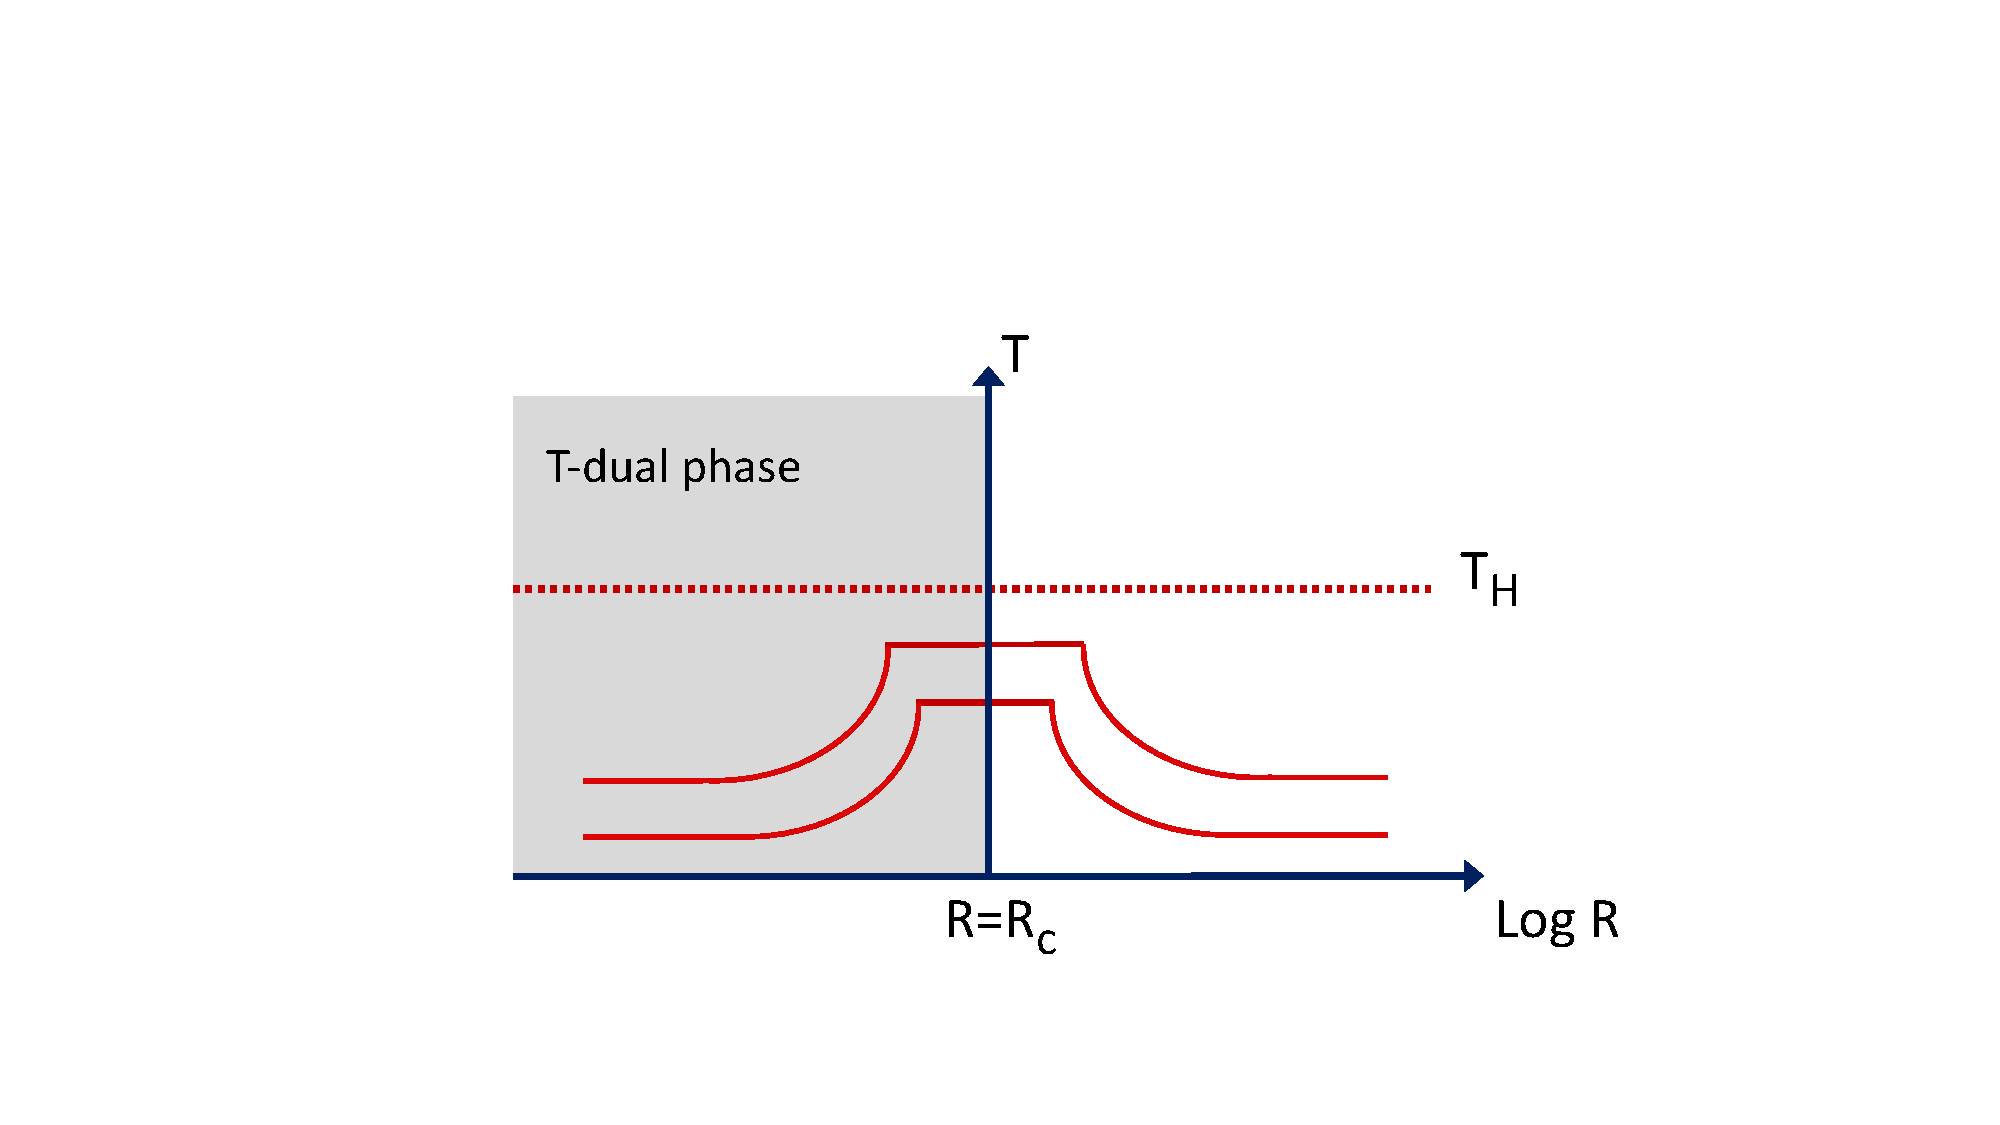
\includegraphics[width=170mm,height=90mm]{Sections/Figures/Hagedorn.pdf} 
 \vskip -25pt
\caption{Temperature $T$ against the radius of the extra dimensions $R$ in string gas cosmology illustrating the Hagedorn temperature as a limiting temperature in string theory and the two dual phases of T-duality separated at the self dual point $R_c$.} \label{Hagedorn} 
\end{center}
\end{figure}

Although these ideas are very attractive, they have been mostly formulated in  simplistic cases for which all of the dimensions are circles. They have not been formulated on realistic set-ups in which chiral matter like in the Standard Model is present. A further issue is that the intuition that strings under tension causes cycles to shrink only holds under the assumption that the dilaton has been stabilised, e.g. by some standard mechanism such as gaugino condensation. This is manifest in 4-dimensional Einstein frame, where the radion is a linear combination of the string frame dilaton and radion.

The lack of understanding of the Hagedorn phase is also a major obstacle at the moment. However, these ideas may eventually be applicable in more realistic frameworks and it is worth to keep them in mind. In particular, after the emergence of the brane-world scenario, generalisation of these ideas may add to the arguments for the critical dimensionality of spacetime. For example, for D4 branes ($p=4$) to avoid annihilating each other they need to live in a universe with dimension greater than $2p+1=9$. This may put a bound on the brane dimensionality to be smaller than four \cite{Burgess:2001fx,Durrer:2005nz}.  A more detailed study for IIB string theory singles out  D3 and D7 branes \cite{Karch:2005yz} which are precisely the branes which host the Standard Model in F-theory and other local D-brane constructions of the Standard Model. For a realisation of inflation making use of the Hagedorn phase see \cite{Abel:2003jh}.

In the regimes where effective field theories are applicable, there also remains the standard challenge of implementing the scenario in realistic set-ups including moduli stabilisation (for a study of a possible realisation in type IIB string theory, see \cite{Frey:2005jk}).

\subsection{Pre Big-Bang Cosmology}

In the 1990s Veneziano and collaborators went beyond the  Brandenberger-Vafa  proposal by considering the possibility of
 $T$ duality in cosmological backgrounds much closer to  the FRW type. For an ansatz  of the type:
$ds^2= -dt^2 + \sum_{i=1}^d a_i^2(t)\ dx_i^2$
it can be seen that $T$ duality is a symmetry of the 
equations of motion acting as:
\be
\setlength\fboxsep{0.25cm}
\setlength\fboxrule{0.4pt}
\boxed{
a_i(t)\rightarrow \frac{1}{a_i(t)},
 \qquad \varphi\rightarrow \varphi - 2 \sum_i\log a_i.
 }
\ee
Since $a_i(t)$ represent the scale factor, as in FRW, this 
has been named {\it scale factor duality} \cite{Veneziano:1991ek}. Thus we can see that expanding and
contracting universes are related by this symmetry.

Gasperini and Veneziano combined this  symmetry with the standard time-reversal symmetry:
$a(t)\leftrightarrow a(-t)$, to allow for a possibility of considering cosmology before  $t=0$, in which the Hubble parameter increases instead of decreases.
Without duality, the symmetry under $t\rightarrow -t$ would send
$H(t)\rightarrow -H(-t)$ but, combining
 this with scale factor duality, it provides four different sign 
combinations for $ H(t)$. 
If the universe at late times is decelerating, $H$ would be a decreasing
 monotonic function of time for `positive' $t$, but a combination of duality
 and the 
$t\rightarrow -t$ transformation can give rise to  $H(-t) = H(t)$ so 
that this
 function can be even, as shown in figure \ref{PreBigBang}. They therefore proposed a scenario in which the universe accelerates from negative times
 towards the big-bang and then decelerates after the big-bang. The 
acceleration would 
indicate a period of inflation before the big-bang without the need of an
 scalar
 potential. This scenario is called {\it Pre Big-Bang Cosmology} \cite{Gasperini:1992em,Gasperini:2002bn,Gasperini:2007vw}, see also \cite{Tseytlin:1991wr}. 

A concrete solution for this system corresponds to the isotropic case
$a_i=a_j\equiv a(t)$ for which:
\be
a(t)= t^{1/\sqrt{d}}\qquad t>0\ , 
\ee
with a constant dilaton. For this solution, $H(t)\sim 1/t$ decreases monotonically 
with time. By applying the transformation $t\rightarrow -t$ and duality we
 can generate the four different branches of solutions:
\be
a(t)=t^{\pm1/\sqrt{d}}\qquad t>0, \qquad a(t)= \left(-t\right)^{\pm1/\sqrt{d}}\qquad t<0, \label{veneziano}
\ee
with 
$\varphi_\pm (\pm t)\ = \ (\pm\sqrt{d} - 1) \log(\pm t)$.

\begin{figure}[t]
\begin{center}
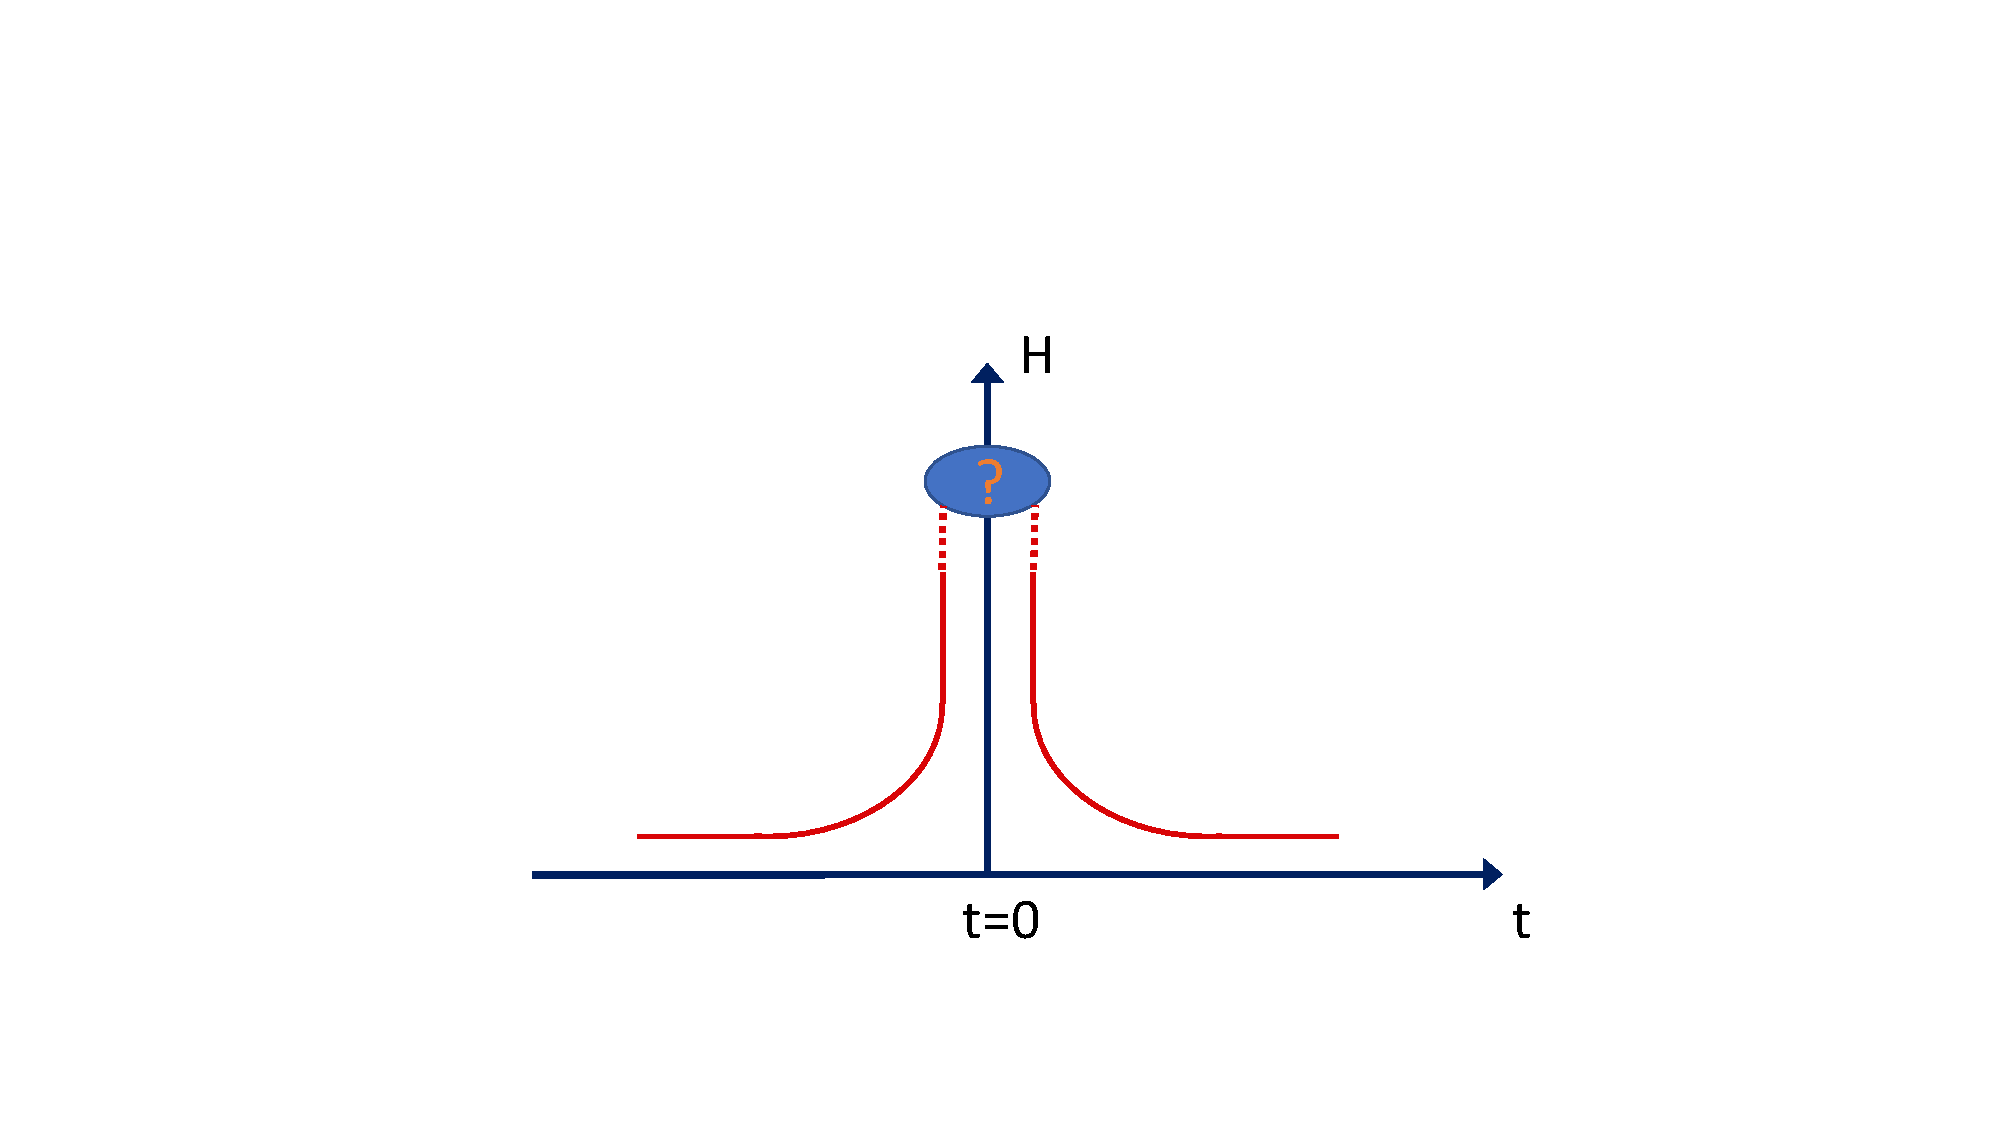
\includegraphics[width=160mm,height=70mm]{Sections/Figures/PreBigBang.pdf} 
\caption{Possible realisation of the pre big-bang scenario with the past and future regions expected to match at the singularity with strong coupling and large curvature.} \label{PreBigBang} 
\end{center}
\end{figure}

In the two branches for which  $H>0$, the universe expands, which provides an 
interesting realisation of the pre big-bang scenario, as illustrated in figure \ref{PreBigBang}.
The solutions are such that there is  a singularity at $t=0$ but also in this
 region the dilaton blows up implying strong string coupling. 
The hope is that non-perturbative string effects provide a smooth 
matching between these two branches. Since the weak 
coupling perturbative string vacuum appears as a natural initial condition 
in the pre big-bang era, the scenario consists of an empty cold
 universe in the infinite past which expands in an accelerated way 
towards a region of higher curvature. Eventually, it approaches the region of 
strong coupling and large curvature, which is assumed will match smoothly
 to the post big-bang branch in which the universe continues expanding but now with
decelerated expansion.

 The spectrum of density perturbations in this scenario has been estimated, and claimed not to contradict the recent 
observations. The scenario also
provides testable differences compared to inflation via the tensor 
perturbations, which could be put to test in future searches for gravitational waves.

While this scenario has very interesting features, it has also been subject to criticism for several reasons. First, as
 the original authors pointed out,
 the main problem to understand is the graceful exit question,
namely how to pass smoothly from the pre to post Big-Bang period. As this requires describing the big-bang singularity, this is a major challenge. 
Close to the Big-Bang the perturbative treatment of 
string theory does not hold since the dilaton and the curvature increase,
 implying strong string coupling. Therefore, there is no concrete way to
 address this issue within the framework where the theory is formulated. 
Another important
 problem is the fact that the moduli are neglected from this analysis and 
there has to be a mechanism that stabilises the extra dimensions. 
Furthermore, the scale factor duality symmetry that motivated the scenario is not
 clearly realised
in  more realistic settings with nontrivial matter content and the fact that the 
dilaton will eventually be fixed by non-perturbative effects may change the 
setting of the scenario. 

On the other hand, this represents an explicit proposal for the early universe with interesting string inputs which  may prove useful in a
more realistic scenario. Furthermore, the study of this scenario has led to interesting potential signatures from gravitational waves and has triggered
much activity in this direction. After the detection of gravitational waves and the future progress in this direction, these preliminary studies of gravitational waves
from a string theory perspective may prove very useful for experimental searches and may be a useful guideline for alternative proposals.

\subsection{Ekpyrotic/Cyclic Scenario}

The ekpyrotic scenario (illustrated in figure \ref{Fig:HW}) was developed in the early 2000s by Khoury, Ovrut, Steinhardt and Turok and has presented itself as an interesting alternative to the inflationary universe, drawing its original inspiration from string theory \cite{Khoury:2001wf,Khoury:2001bz,Steinhardt:2002ih, Lehners:2008vx}.

The proposal was first formulated within a particular string theory scenario, namely the 11-dimensional formalism of Horava and Witten with one of the dimensions compactified in an interval $I$ (understood as a $Z_2$ orbifold of a circle $I=S^1/{\bf Z}_2$). 
The endpoints of the interval correspond to two parallel 10-dimensional spaces or {\it end of the world branes}  
which are the `fixed points' of the orbifold, with each hosting $E_8$ gauge theories, providing a strong coupling version of the heterotic string.
 Further compactification on a six-dimensional Calabi-Yau manifold then leaves two 
4D worlds at the ends of the interval in the 5D bulk. In principle, quasi-realistic
 models can be obtained from this approach, mostly using the topological
 properties of Calabi-Yau manifolds. It turns out that besides the end
 of the (interval) 
world branes, which we may also refer to as boundary  branes,
 there are also five-dimensional branes in these compactifications (M-branes) that are not restricted to
live at the fixed points and can move through the bulk.
 These are called bulk branes in order to differentiate them from the boundary branes. Overall, these
 configurations are reminiscent of models with both D-branes at orbifold singularities and also mobile branes.

\begin{figure}[t]
\begin{center}
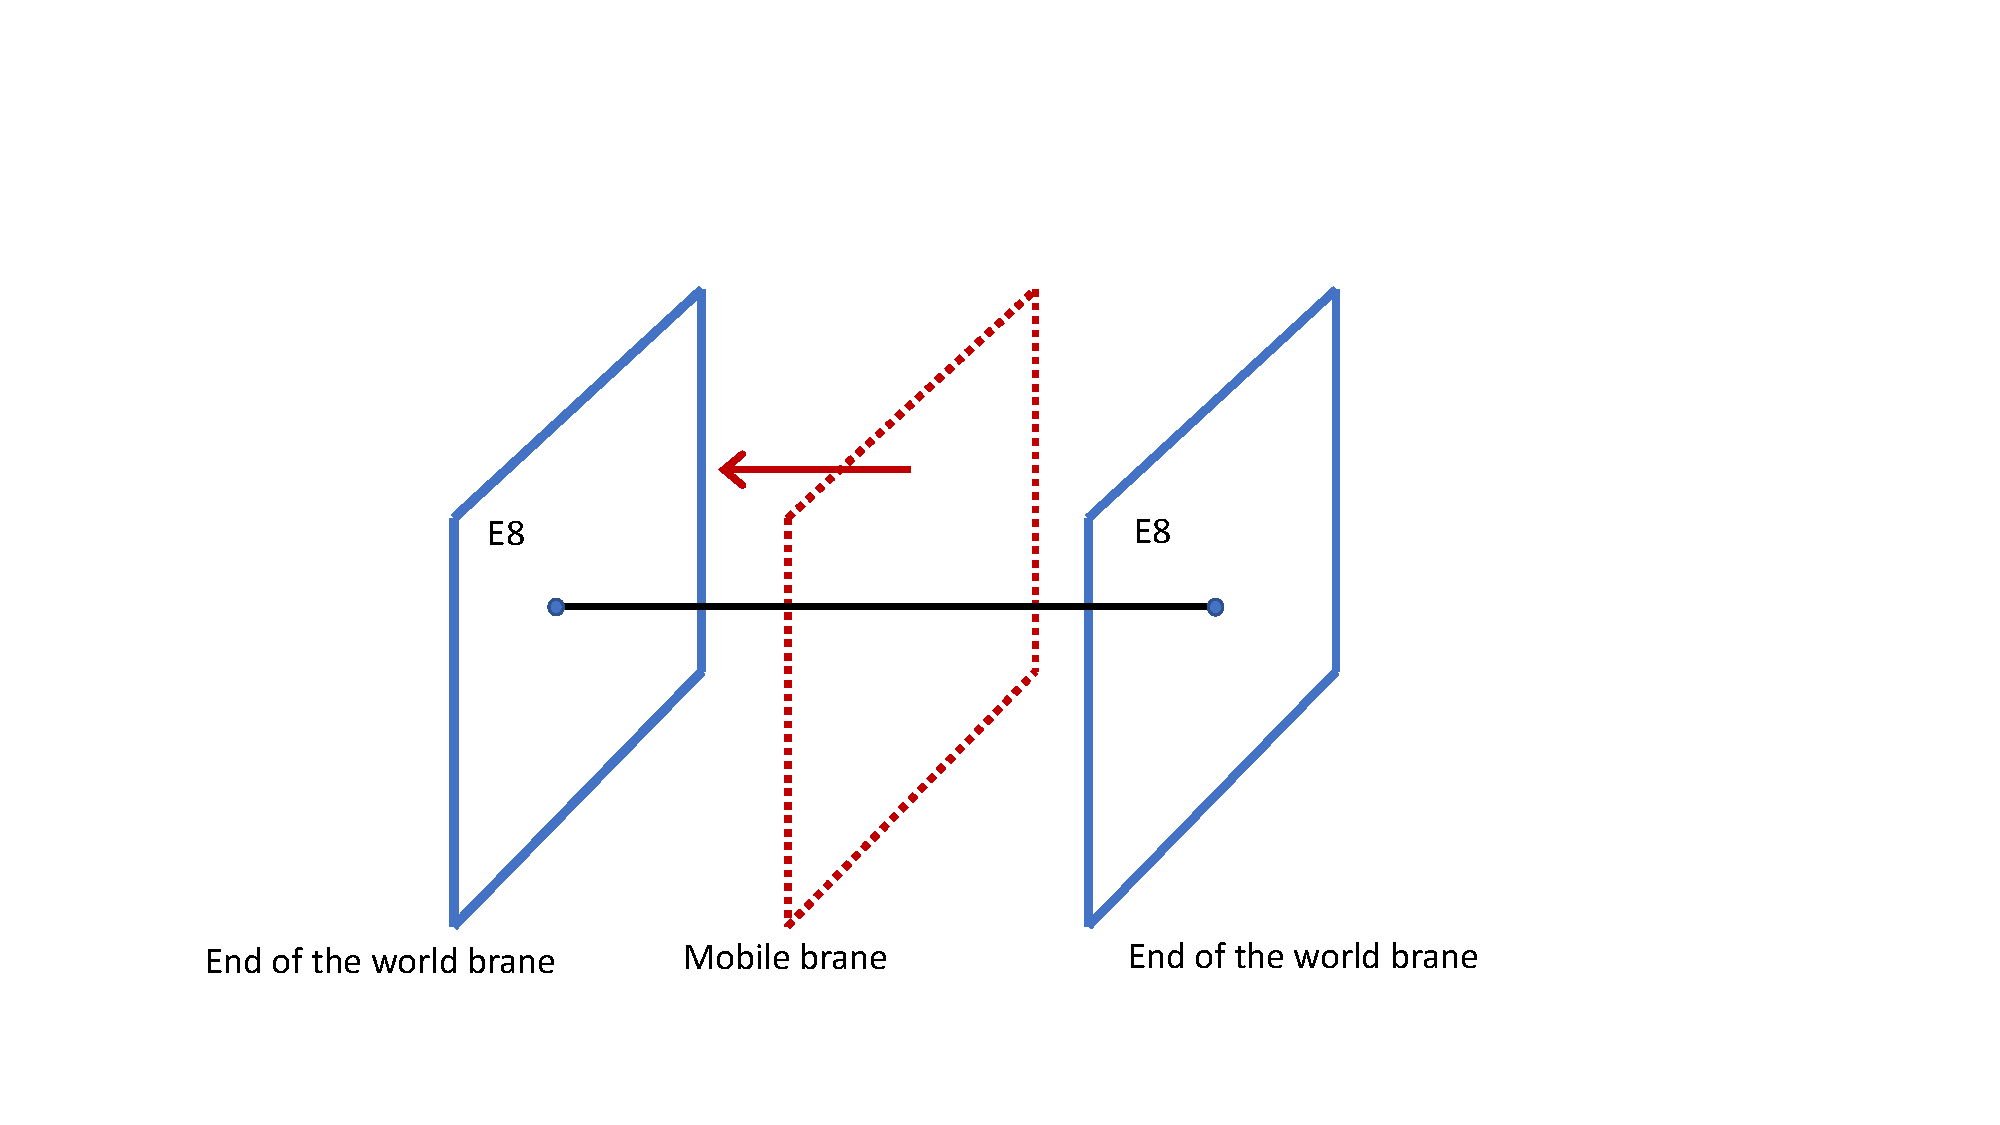
\includegraphics[width=150mm,height=90mm]{Sections/Figures/Horava.pdf} 
\caption{The Horava Witten scenario. 
Two surfaces or end of the world branes, each at the end of 
the interval, provide chiral matter and possibly interesting cosmology as proposed in the ekpyrotic/cyclic scenario. Ripples on the mobile brane may be the source of density perturbations.} \label{Fig:HW} 
\end{center}
\end{figure}

Khoury {\it et al.~} also made an interesting proposal regarding the collision of branes, not to obtain inflation as in the brane inflation discussed in section \ref{sec:infla}, but as an alternative to inflation. The original idea
was to assume that a (hidden) bulk brane going from one boundary of the interval to the other end, would collide with the second (visible) boundary 
brane and produce the Big-Bang. The bulk brane would be almost BPS -- by which it was 
meant that it is essentially parallel to the boundary branes --  and move freely and slowly from one end of the interval to the other.
Small quantum fluctuations  induce some ripples on this brane which, when colliding with the visible end of the world 
brane, would produce the density fluctuations measured in the CMB. There is 
no need of an inflation potential for this. A potential of the type 
$-e^{-\alpha Y}$, with $Y$ is the separation of the branes, was proposed, although not derived, describing  the attraction of the branes. 
The 5D metric is taken with a warp factor that implies that the
motion is
 from smaller to larger curvature across the interval and therefore the scale 
factor depends on the position of the brane in the interval. 

This proposal has received several critics The first involves 
the standard problems solved by inflation. The horizon and flatness
problems require the  branes to be almost exactly parallel before collision,
which may require a fine-tuning of initial conditions. Although relics such as
monopoles will not be present if the collision temperature is low
enough this argument needs to be properly quantified. There is also no general natural
dilution, as in the exponential expansion of inflation, making the solutions of these problems more
difficult in general.  The issue of fine tuning of
 the initial conditions in the ekpyrotic scenario has been widely debated.

However, the most prominent difficulty of this scenario is the following:
in a 4D description, $\dot a<0$ before the collision, while it is expected that $\dot a>0$ after the collision,
 which requires a transition from contraction to expansion, without, in principle, crossing a 
singularity. This is a problem because it violates the null energy condition.

Let us briefly review this argument. Consider gravity coupled to a scalar field: (setting $\kappa_5=1$) 
\be
{\cal L}\ = \ \sqrt{-g}\left( R-\frac{1}{2} 
\partial_\mu\phi\partial^\mu\phi-V(\phi)\right),
\ee
The energy density and pressure are given by:
\be
\rho\ = \ \frac{1}{2}\dot\phi^2 + V, \, \qquad p\ = \ \frac{1}{2}\dot\phi^2 - V .
\ee
Therefore, Einstein's equations imply:
\be
\setlength\fboxsep{0.25cm}
\setlength\fboxrule{0.4pt}
\boxed{
\dot H =  -\frac{1}{2}\left(\rho+p\right) = 
-\frac{1}{2}\dot\phi^2 \leq \ 0.
}
\ee
This implies that $H$ is  monotonically decreasing and 
we cannot go from contraction ($H<0$) to expansion ($H>0$).

This problem motivated a second version of this scenario 
 which does not include the mobile brane but considers the collision of the two end-of-the-world branes. In this case, there is 
a singularity at the moment of collision, since the size of the fifth dimension reduces to zero, 
 which, in principle, could allow a transition from 
contraction to expansion. The singularity happens only in the extra dimension because the scale 
factors of the branes remain finite during the process. After the collision, the two branes separate again and the scale factor increases (see Fig. \ref{F:ekpyvar}).
\begin{figure}[t]
\begin{center}
\vskip -10pt
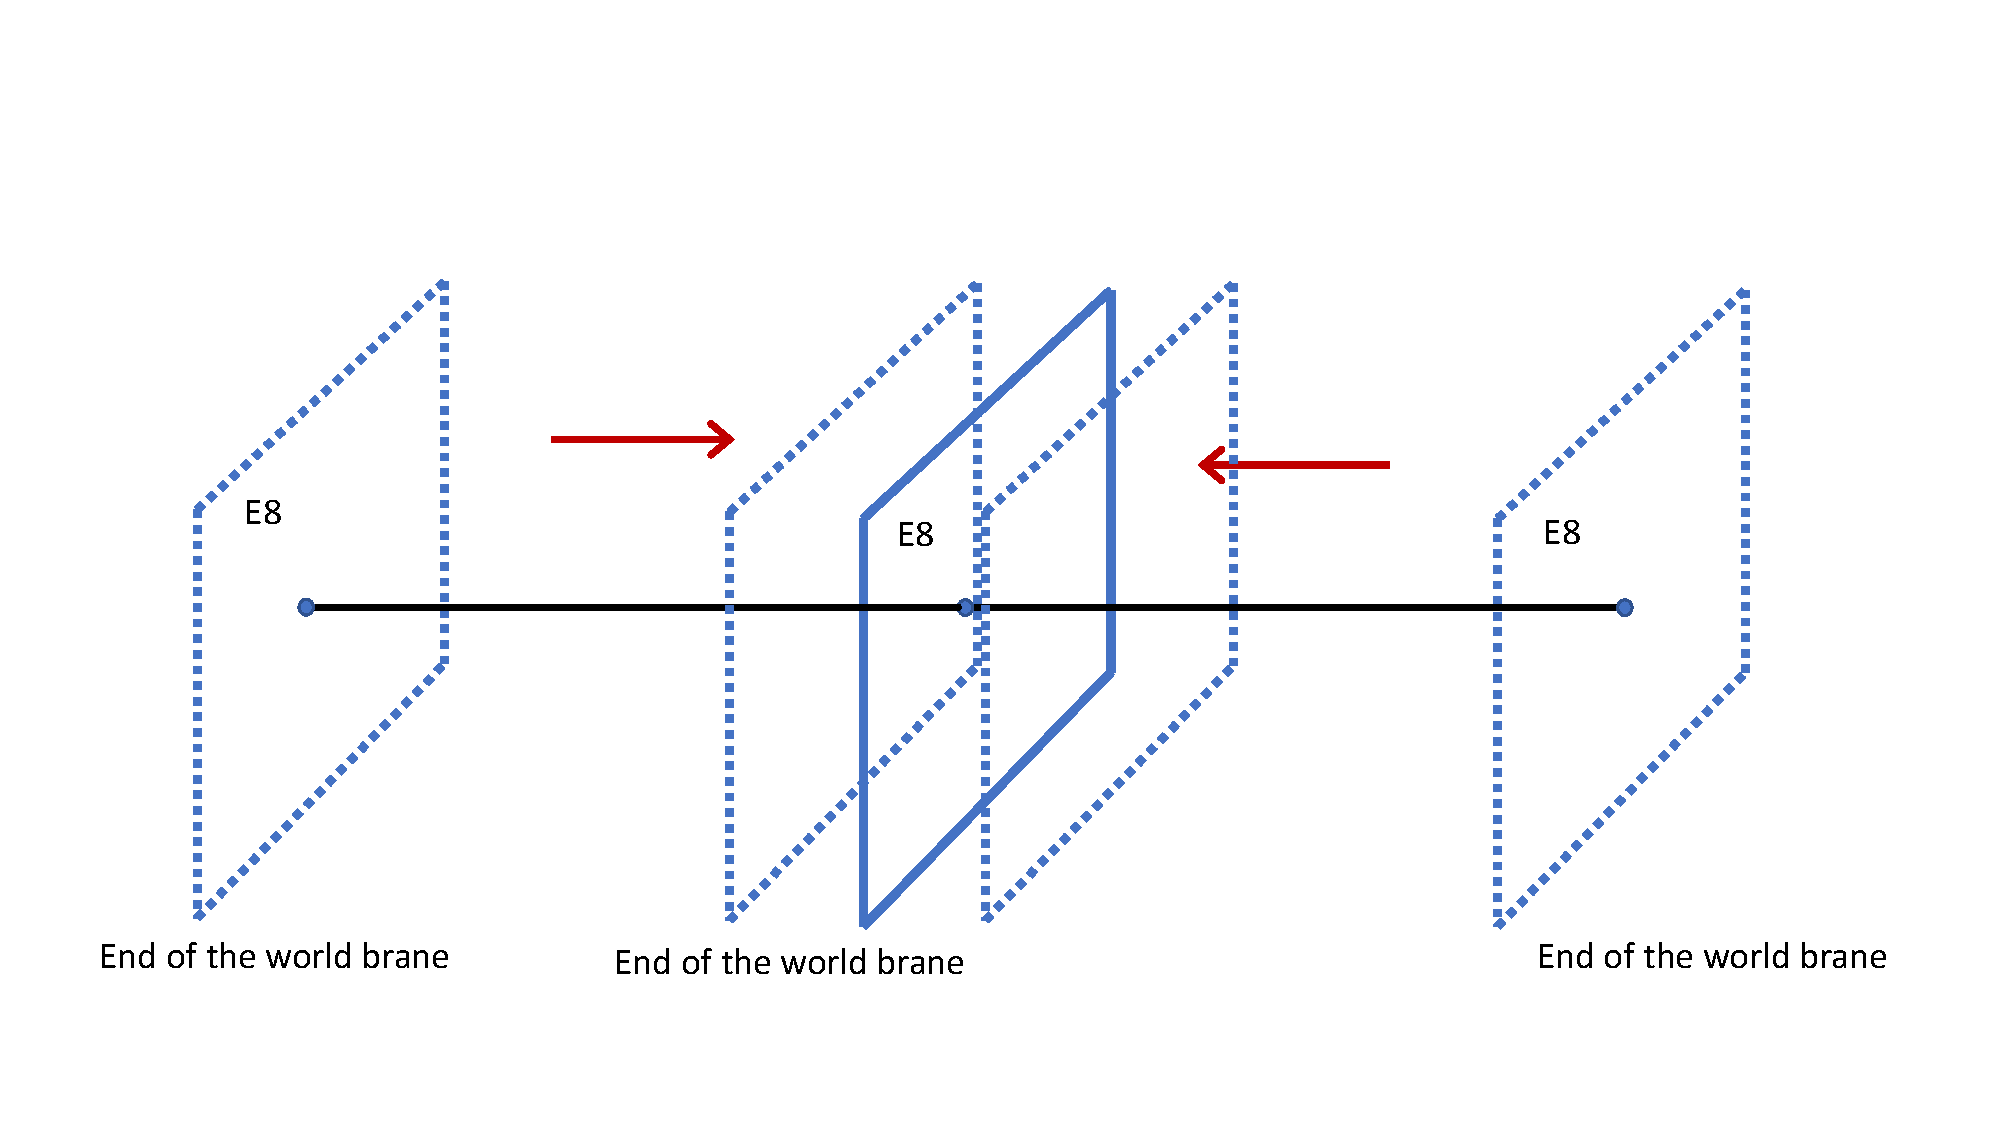
\includegraphics[width=140mm,height=90mm]{Sections/Figures/Cyclic.pdf} 
\caption{A variation of the original ekpyrotic universe scenario in which the end-of-the world branes approach each other, pass through their overlap point and at some point return, so completing the cycle.} \label{F:ekpyvar}
\end{center}
\end{figure}

In terms of a four-dimensional EFT,  this process can be understood in similar terms to the discussion of the
 Pre Big-Bang proposal. Neglecting the scalar potential and identifying  the separation between the branes with 
 the string dilaton (as it happens in the Horava-Witten scenario) we can use equations (\ref{veneziano})
for the case $d=4$. Out of the four possibilities provided by the choices of sign we can choose:
\be
a(t)\ = \ |t|^{1/2}, \qquad \phi\ = \ \phi_0\pm \sqrt{3}\log|t|.
\ee
The  scale factor $a(t)$ goes from contraction
at negative $t$  to expansion at positive $t$. This still leaves the choice of sign for the 
dilaton open. Since the string coupling is proportional to 
$e^{-\phi}$, the negative sign  choice that was taken in the pre big-bang scenario
corresponds to strong string coupling whereas the positive choice, 
chosen in the ekpyrotic scenario, implies weak coupling at $t=0$. Therefore 
Khoury and collaborators conjectured that the transition is smooth at the singular point and  afterwards the branes may start to separate again. 



This leads us to a third version of this scenario that corresponds
 to the {\it cyclic universe} \cite{Steinhardt:2002ih}. In this case, the two branes keep separating and
 passing through each other an infinite number of 
times, as long as the interacting 
potential has a very particular form. For instance, for a potential like that of
 Fig. \ref{Fig:cyclic}, we may describe the universe's history by starting on the right
 hand side corresponding to the current time. The potential is taken to be slightly positive 
and with a slightly negative slope, reflecting the fact that the universe accelerates today as in quintessence.

 Since the slope of the potential is  negative, the scalar field
will start rolling towards smaller values representing the higher dimensional picture of the branes approaching each other.
At some point the field will cross the $V=0$ point and its energy density
 will mostly be kinetic. The potential rapidly becomes negative
 and then the energy density $\rho= V+\frac{1}{2}\dot\phi^2$ touches zero, implying 
that the universe starts contracting. Since the kinetic energy is also 
large, the 
field  passes through the minimum, towards the flat region at infinite
$\phi$ or zero string coupling, where the branes collide
and bounce back with enough energy to re-cross the steep minimum and
go to the right hand side of the 
potential, where it returns to a radiation dominated era,before repeating the
whole cycle again.
\begin{figure}[t]
\begin{center}
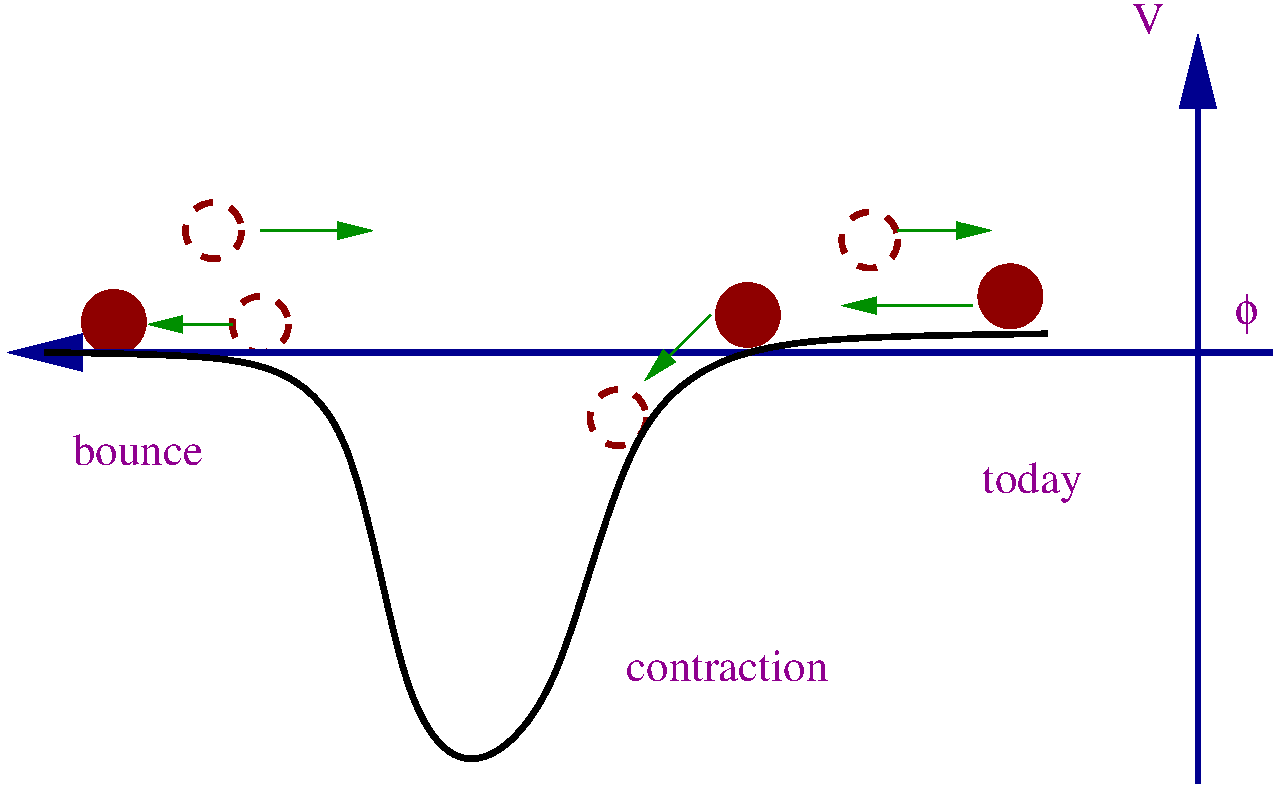
\includegraphics[width=100mm,height=60mm]{Sections/Figures/cyclic2.pdf} 
\caption{An illustration of the potential and
 trajectory of the field in the cyclic universe. Figure taken from  \cite{Quevedo:2002xw}. } \label{Fig:cyclic} 
\end{center}
\end{figure}

The different versions of this scenario claim to resolve the same questions addressed by inflation. 
For instance, the claim is that the horizon problem does not exist if there is a bounce, since there will be
 clear causal contact between different points. In the cyclic version,
the late period of mild inflation plays a similar role as the
original inflationary scenario by dissolving unwanted objects such as 
like magnetic monopoles, and emptying the universe for the next cycle, thereby also solving the
flatness problem.
 Furthermore, the spectrum of perturbations has been claimed to be 
consistent with observations. Although this issue has been debated, 
all parties seem to agree that the methods used so far are not entirely
conclusive one way or another.

There are some  interesting aspects to these proposals, 
especially regarding  the revival of the cyclic universe. A cyclic universe was originally proposed in the 1930's 
but it was immediately realised that the entropy increases on each cycle, requiring the length of
each cycle to increase. Extrapolating back in time, we reach 
an initial singularity rendering the model only semi-eternal,
similar to eternal inflation which also requires a beginning. So it is not really cyclic.

In the current version, the old entropy problem is claimed to be solved as follows. Although it is true that the total entropy 
 increases with each cycle, the entropy of matter is always the same 
at the end of each cycle. This is due to the present accelerated expansion
 which dilutes matter and so renders the universe essentially
 empty, actually one particle per Hubble radius, before restarting the cycle.
This scenario was found in the context of the ekpyrotic scenario,
but it is clearly independent of it and may have other  realisations.

Another interesting point of this scenario is that it connects the early
 universe and 
late universe in a coherent way. The current acceleration is used as a way 
 to prepare the universe to the next cycle.

 
Even though the scenarios were motivated in terms of string theory, the 
kind of scalar potentials that are needed for this scenario to work are relatively contrived and have not been 
derived from the underlying theory.
 This is certainly an important  question to be addressed before these models 
can be considered genuine string/M-theory models. In this sense, these scenarios are 
 presently at a similar stage as D-brane inflation was in 1998 where the scalar 
potential was only guessed, rather than explicitly calculated as in the 
brane/antibrane \cite{Burgess:2001fx, Kachru:2003sx}. 
Finding a potential with the 
proposed properties represents a clear open challenge for these models.
 
From a string theory perspective, there are several other problems with this scenario. 
In particular, the assumption that 
the moduli of the Calabi-Yau manifold are fixed and decoupled is not justified.
 Nonetheless, the main problem to deal with remains the big-bang singularity 
giving rise to the bounce. This is a strong assumption as description of the bounce relies on strong coupling and non-perturbative dynamics.
For further developments regarding the implementation of the ekpyrotic scenario see \cite{Buchbinder:2007ad}. For a comprehensive review of the subject see \cite{Lehners:2008vx}.


\medskip
In summary, what the three scenarios: of pre big-bang cosmology, string/brane gas cosmology and ekpyrotic/cyclic have in common is that they
contemplate a period of contraction, and represent examples of bouncing cosmologies.
For a nice recent review on such bouncing cosmologies, see \cite{Brandenberger:2016vhg}.

\subsection{The Rolling Tachyon}

As we have seen in section \ref{sec:infla} the open string tachyon plays an important role in brane anti-brane inflation. It provides the natural way to end inflation and is the source of production of lower dimensional branes like stringy cosmic strings.

From the formal perspective, there has been concrete progress in understanding from first principles the physics of the open string tachyon. In particular, using string field theory Sen managed to extract substantial information regarding the tachyon potential \cite{Sen:2002nu} (for a review see \cite{Sen:2004nf}). This is actually one of the only cases in which a scalar potential has been derived directly from string theory. It is therefore worth exploring the potential cosmological implications of the tachyon field, independent of brane inflation.
 
String calculations suggest that to all orders in derivative expansion these actions take a Born-Infeld form.
\be
\setlength\fboxsep{0.25cm}
\setlength\fboxrule{0.4pt}
\boxed{
{\cal L}\ = -\ V(T)\ \sqrt{1- g^{\mu\nu} \partial_\mu T \partial_\nu T}\ ,
}
\ee
where $V(T)$ can take different forms depending on the type of string theory, 
namely bosonic or supersymmetric. 

First, Sen studied the rolling of the tachyon to its asymptotic minimum 
$T\rightarrow \infty$ and concluded that, even though the vacuum should correspond to the closed string vacuum and the unstable D-brane system 
(such as brane/antibrane pairs or non BPS D-branes) has decayed, the energy density is still localised. Furthermore, 
he was able to prove that the resulting gas corresponds to a pressure-less gas. This is easy to see from the
effective action above for which the stress energy tensor
for a time-dependent tachyon implies
\be
\rho\ =\ \frac{V(t)}{\sqrt{1-\dot T^2}}\ , \qquad p\ =\ -V(T)\sqrt{1-\dot T^2}
\ .
\ee
 For constant energy density, the pressure behaves as $p=-V^2/\rho$ and at the
 minimum in $T\rightarrow \infty$ we know that $V\rightarrow 0$ and so 
$p\rightarrow 0$. The equation of state is $p= \omega\,\rho$ with $\omega=-(1-\dot T^2)$ and therefore
$-1\leq \omega\leq 0$.

For a time-dependent tachyon field, we should actually consider a time-dependent metric such as the one of  FLRW. 
In \cite{Gibbons:2002md} this was done, obtaining the 
Friedmann's equations for this Lagrangian coupled to 4D gravity:
\begin{subequations}
\begin{empheq}[box=\widefbox]{align}
H^2 & =  \frac{8\pi G}{3} \frac{V(T)}{\sqrt{1-\dot T^2}} - \frac{k}{a^2}\ , 
\nonumber \\
\frac{\ddot a}{a} & =   \frac{8\pi G}{3} \frac{V(T)}{\sqrt{1-\dot T^2}}
\left(1-\frac{3}{2} \dot T^2\right)\ .
\end{empheq}
\end{subequations}
Even without actually solving these equations, it can be easily seen that the
energy density decreases with time, while $T$ increases relaxing towards the
 asymptotic minimum of the potential. In the meantime the universe expands,
first accelerating ($|\dot T|<2/3$) and then decelerating ($|\dot T|>2/3$).
Depending on the value of the spatial curvature
 $k=0,1,-1$, the scale factor $a(t)$ goes to a constant for $k=0$, 
to a Milne universe $a(t)\rightarrow t $ for $k=-1$ or re-collapses, for 
$k=1$.

Another natural question is whether
this tachyonic potential can give rise to
 inflation by itself. However, this is challenging
The main reason is the absence of small parameters in the potential 
that can be tuned to give a sufficiently slow roll. See however \cite{Padmanabhan:2002cp,Frolov:2002rr,Fairbairn:2002yp,Cremades:2005ir}.

As well as open string tachyons, string spectra can also include tachyons in the closed string spectrum.
The situation with closed string tachyons is more complicated and less understood. One way to 
see this is that, while the open string tachyon triggers the disappearance of D-branes after their collision 
by settling to the minimum of the potential, closed string tachyons are intrinsically gravitational and so their condensation 
may represent the disappearance of spacetime itself. Some simplifying configurations have been studied in which this happens for localised regions of spacetime that somehow mimics the open string case but the general case
is not fully understood. This is also related to the fact that string field theory is better understood for open strings than for closed strings. For a detailed discussion
of some phenomenological aspects see e.g  \cite{Adams:2001sv,Choudhury:2002xu, Shiu:2002qe} and for comprehensive review on tachyon dynamics including cosmological implications see \cite{Sen:2004nf}.

\subsection{S-Branes}

 Closely connected to the rolling tachyon is the concept of an {\it S-brane} \cite{Gutperle:2002ai}. An S-brane is a topological defect for which 
all longitudinal dimensions are spacelike, and so it  exists
 only for an instant of time. There are several reasons to introduce these 
objects.  The simplest example  in field theory corresponds to 
a  potential for a real scalar field of the standard double-well form:
\be
V(\phi)\ = \lambda \left(\phi^2 - a^2\right)^2\ , 
\ee
with minima at $\phi_{\pm}=\pm a$. In 4D this has the standard domain wall solution $\phi(x)=a\tanh(\sqrt{2\lambda}ax)$  or 2-brane
topological defect interpolating between the regions where the field is in 
the
$\phi_+$ and $\phi_-$ vacua. 

For S-branes, we have a time-dependent configuration in which we start at the maximum 
of the potential  $\phi(x,t=0)=0$
but with nonzero velocity $\dot\phi(x,t=0)=v>0$. This will make the field  roll towards $\phi_+$, until it oscillates and eventually 
arrives at the minimum. A time reversal situation would have the field starting in $\phi_-$ and going to $\phi=0$. 
We can then have  the field evolving from $\phi_-$ at $t=-\infty$ to $\phi_+$ at $t=\infty$ looking like a kink in time and filling all spatial dimensions. This is an S2 brane. This  process requires some fine tuned exchange of energy in order for the field to climb the barrier.

Using the analogy with D$p$-branes, we expect that the S$p$-branes can
also be found as explicit solutions of Einstein's equations
 coupled to dilaton and antisymmetric tensor fields. 
 
We start with the Lagrangian for the metric, dilaton, antisymmetric tensor $F_{q+2}= 
dA_{q+1}$  (and setting $\kappa_p=1$),
\be
\setlength\fboxsep{0.25cm}
\setlength\fboxrule{0.4pt}
\boxed{
{\cal L} \ = \ \sqrt{-g}\left( R-\frac{1}{2} 
g^{\mu\nu}\partial_\mu\varphi\partial_\nu\varphi-\frac{1}{2(q+2)!}
 F_{q+2}^2\right).
\label{einstein}
}
\ee
The equations of motion have solutions similar to the ones found for black branes. 
In the same way  that $p$-brane solutions
are black hole-like, we expect that S-brane solutions correspond to
time-dependent backgrounds of the theory, and therefore may have a  cosmological interpretation. This is actually the case. 

The simplest example can be obtained for pure gravity. Starting with  the Schwarzschild solution in 4d corresponding to a black hole of mass $M$ we can perform the following analytic continuation:
 \be
 t\rightarrow ir,\qquad  r\rightarrow it, \qquad
 \theta\rightarrow i\theta, \qquad \phi\rightarrow i\phi
 \ee
  together 
with $M\rightarrow iP$. The metric becomes
\be
d\hat s_I^2\ = \ -\left[1-\frac{2P}{t}\right]^{-1}\ dt^2\ + 
\ \left[1-\frac{2P}{t}\right] \ dr^2\ + \ t^2\ \left(\sinh^2\theta\ \ 
d\phi^2\ + \ d\theta^2\right), 
\ee
whose surface of constant $r$ and $t$ is now the 
hyperbolic plane ${\cal H}_2$ rather than the two-sphere, consistent with the time-like nature of the S-brane. 

In addition to the symmetries of the hyperbolic space, the solution has
a spacelike Killing vector $\xi=\partial_r$ but is now time-dependent, 
again, as expected for a S-brane. The apparent singularity at $t=2P$ is
 again a horizon. For $t<2P$ the metric is:
\be
d\hat s_{II}^2\ = \ -\left[1-\frac{2P}{r}\right]\ dt^2\ 
+ \ \left[1-\frac{2P}{r}\right]^{-1} \ dr^2\ + \ r^2\ \left(\sinh^2\theta\ \
d\phi^2\ + \ d\theta^2\right), 
\ee
which is now static with a time-like singularity at $r=0$. The corresponding Penrose diagram is a $\pi/2$ rotation of the Schwarzschild black hole diagram as can be seen in figure (\ref{sbrane}).

\begin{figure}[t]
\begin{center}
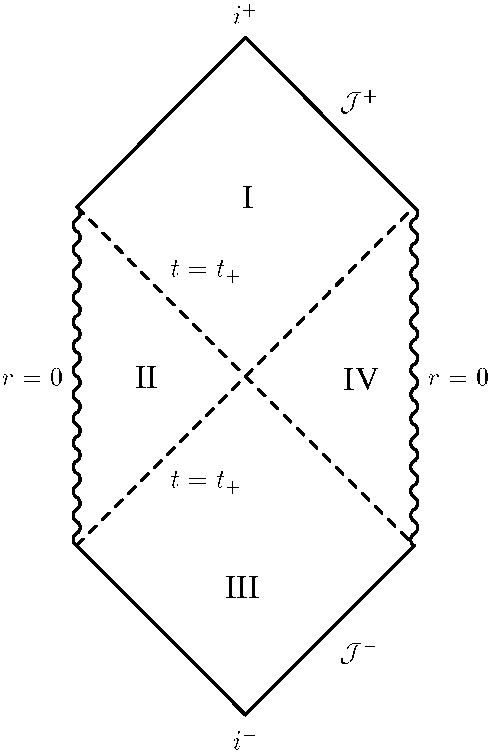
\includegraphics[width=55mm,height=80mm]{Sections/Figures/sbrane.pdf} 
\caption{Penrose diagram for an S-brane. Note that this is a $\pi/2$ rotation of the Schwarzschild black hole Penrose diagram. Regions I and III are cosmological, representing expanding and contracting cosmologies, respectively, separated by smooth horizons which are identified with the S-brane. Regions II and IV are static and have time-like singularities, which can be identified with negative tension end-of-the-world brane-like objects similar to orientifolds. Their corresponding mass and charge can be computed explicitly.} 
\label{sbrane}\end{center}
\end{figure}

More general solutions  of (\ref{einstein}) will have both dilatonic  and  $F_{q+2}$ charges (see for instance \cite{Grojean:2001pv,Burgess:2002vu}). 
The static region provides us with a way to  identify 
this geometry correctly. It turns out that the singularities are the
 physical objects  to which mass, or tension and charge can be
 assigned unambiguously.
It was found that the two singularities correspond to negative tension 
objects, like end-of-the-world branes with opposite charge. 
Furthermore, the similarity with black
hole geometry 
indicates that there will be particle production 
 and we 
 can also compute a generalised Hawking temperature and entropy which could have 
interesting cosmological interpretations. Finally, just as in the case of the Pre Big-Bang, ekpyrotic/cyclic and brane gas scenarios, S-branes naturally have a period of contraction of the universe corresponding to region III of the Penrose diagram, followed by another period of expansion (region I). For further details on the cosmological interpretations of S-branes see for instance \cite{Grojean:2001pv,Burgess:2002vu,Cornalba:2002nv,Cornalba:2002fi,Burgess:2003tz,Kounnas:2011gz,Townsend:2003fx,Ohta:2003pu}.




\subsection{Swampland Conjectures}
\label{Sec:Swamp}

\begin{figure}[t]
\begin{center}
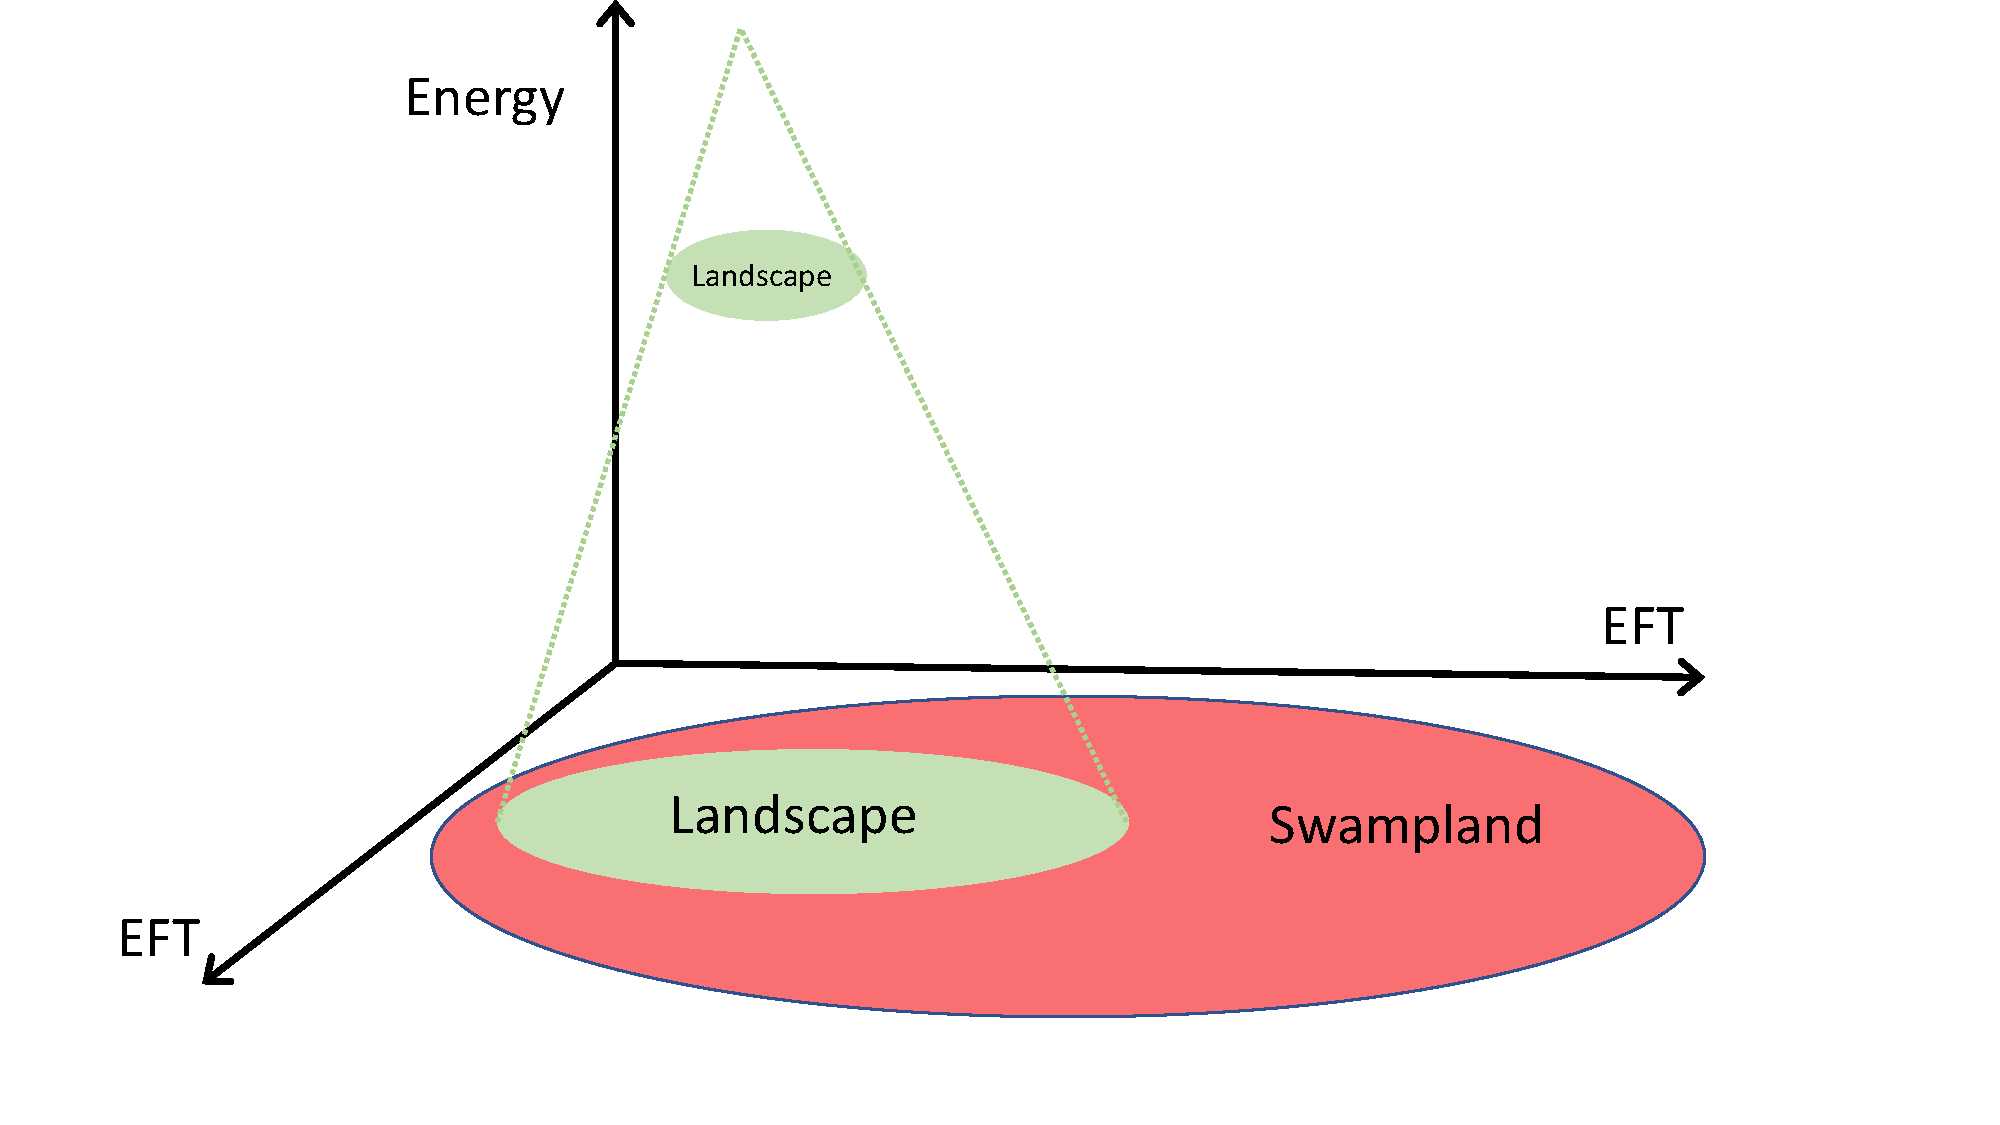
\includegraphics[width=140mm,height=90mm]{Sections/Figures/Swampland.pdf} 
\caption{A cartoon representation of the swampland. At low energies there are many consistent effective field theories, but only a subset of them can be lifted to be UV complete inside a quantum gravity theory. These correspond to the landscape. The rest  are referred to as the swampland.} \label{swampland}
\end{center}
\end{figure}

The vast number of apparent string vacua has very interesting implications. As described in Chapter \ref{sec:DE}, it may be the only self-consistent way to explain the smallness of the dark energy and may provide a totally different approach to asking fundamental questions in physics, separating the `interesting questions' (those that do need an explanation from an underlying theory) from the `uninteresting questions' (those that may be explained by the presence of the multiverse). However, this may also lead to the belief that any theory at all may be derivable from string theory, resulting in a conclusion that it is impossible ever to test string theory, even in principle. This gives the idea of the swampland, illustrated in figure \ref{swampland}.

That said, since the early days of string theory we have known that this is not true: there are some, albeit only a few, general physics properties that can be extracted from string theory. Namely,
\begin{itemize}
\item The need for supersymmetry at the fundamental level (although the scale of its breaking is not known and it may take non-standard forms as in misaligned supersymmetry \cite{Dienes:1994np});
\item
 The existence of extra dimensions, and more concretely only 6 or 7 extra dimensions; 
 \item 
 The existence of moduli fields with specific properties, in particular gravitational-strength couplings, 
 which appear in very specific ways within the low-energy effective field theory; 
 \item The absence of an infinite number of continuous spin representations corresponding to massless particles. These are in principle allowed by the principles of quantum mechanics but have not been observed in nature, despite the lack of alternative explanations from basic principles;
 \item The general absence of global symmetries in the effective field theory.
\end{itemize}

These general results can be complemented with general properties of the landscape, for instance, if the landscape is dominated by Coleman-de Luccia vacuum transitions, a general claim exists that the curvature of the Universe has to be negative, implying an open universe. However, the power of such general results is limited and they still allow for the existence of the enormous landscape resulting in limited predictive power.

In the past few years a new approach towards addressing concrete questions from string theory has been developed and comes under the name of {\it swampland conjectures} \cite{Vafa:2005ui}. The idea is very simple: exploit our cumulative experience of string vacua to extract results that may actually be general. This program aims to state concrete conjectures whose validity may be tested through further exploration of string solutions, either to confirm or rule out the conjecture. The overall goal of the swampland conjectures is:

\begin{quotation}
\emph{Identify which effective field theories are consistent at low energies but cannot be consistent in a UV completion of the theory including gravity.}
\end{quotation}

This is a modern version of what used to be known as {\it vacuum cleaning} in the sense of having a systematic procedure to separate the proper vacua from those that cannot be UV completed. Such conjectures can be made much sharper by going beyond string theory and claiming that the corresponding conjectures will hold for {\it any} theory of quantum gravity, string theory or otherwise. In this sense, string theory is used only to identify the corresponding conjectures, while the swampland approach aims not only to select string vacua, but to identify general properties of any theory of gravity.


More generally, the study of UV constraints on IR physics is a  blooming field that has seen many new conceptual and technical developments recently.
While the swampland programme is one of these developments,  it is worth mentioning a powerful approach, which simply assumes  unitarity, locality, causality, and Lorentz invariance of the, otherwise unknown, UV completion to derive  constraints on the effective field theories, (see \cite{deRham:2022hpx} for a recent overview on these ideas). Combining these approaches may bring the swampland programme to a firmer footing, for example via positivity bounds or bootstrap arguments. 

Over the years, a range of swampland conjectures have been put forward. They range between those that are strongly motivated, but with limited phenomenological or cosmological impact, to conjectures that may have a major impact, but which lack a robust basis and may be considered extremely speculative. There are several excellent reviews on this field in which a detailed discussion of the conjectures has been explained and argued in much detail \cite{Brennan:2017rbf,Palti:2019pca,vanBeest:2021lhn, Grana:2021zvf} to which we refer the reader for further details and the majority of the original references. Here we content ourselves by briefly mentioning those conjectures that could be more relevant for cosmology:

\begin{enumerate}
\item{\it Absence of global symmetries}. A consistent theory of gravity with finite number of states cannot have exact global symmetries. General arguments in this direction have existed since the 1980s: both through arguments that -- contrary to local symmetries -- global symmetries are not protected by black holes after radiation, and also that within string theory, a conformal field theory that leads to a global symmetry also leads to a massless particle in the spectrum that corresponds to the gauge field of that symmetry and therefore the symmetry is not global but local in spacetime \cite{Banks:1988yz}.  More recently, further evidence has accumulated to support its validity. While the general impact of this result is strong, it provides only weak constraints on local symmetries with very weak couplings that to most practical particle physics purposes behave as global symmetries (see for instance \cite{Burgess:2008ri}).

\item {\it Weak gravity conjecture \cite{Arkani-Hamed:2006emk}}. The observational fact that we observe gravity to be the weakest force may not be a property only of our Universe but also of any possible universe described by a consistent theory of gravity. A concrete statement of this conjecture is that in any consistent theory of gravity, there should exist a particle of charge $Q$ and mass $M$ such that $Q^2>GM^2$ (for which the Coulomb force is stronger than the Newtonian force) although more precise and generalised formulations have been proposed \cite{Harlow:2022gzl}. This is the prime example of a  swampland conjecture  that has been argued and tested in sufficiently many ways that there exists a broad consensus that it is actually a correct statement. This has played a useful role in cosmology, especially when extended to forces mediated by scalar fields and  antisymmetric tensors, and in particular when they are dual to axion-like-particles. The weak gravity conjecture may also then be used to constrain the axion decay constant that plays a role in some models of inflation.

\item{\it Cobordism conjecture \cite{McNamara:2019rup}.} Two manifolds are called cobordant if their union is the boundary of another manifold of one extra dimension. This defines an equivalence relation. The corresponding equivalent classes may define a global (topological) charge. We may generalise the absence of global charges conjecture to this topological case and conjecture that  in  a consistent theory of gravity, all cobordism classes have to be trivial. If the corresponding manifolds are, for instance, the 6-dimensional compact spaces, the corresponding 4-dimensional EFTs would be separated by a domain wall (see figure (\ref{cobordism})). If the cobordism class is trivial then it must admit  an end-of-the-world configuration as in the Horava-Witten or bubble of nothing cases (see figure (\ref{cobordism2})). If this conjecture holds, it may have very important implications for cosmology due to the presence of the boundary-ending spacetime. For recent developments in this direction see for instance \cite{Angius:2022aeq,Angius:2022mgh}.

\begin{figure}[t]
\begin{center}
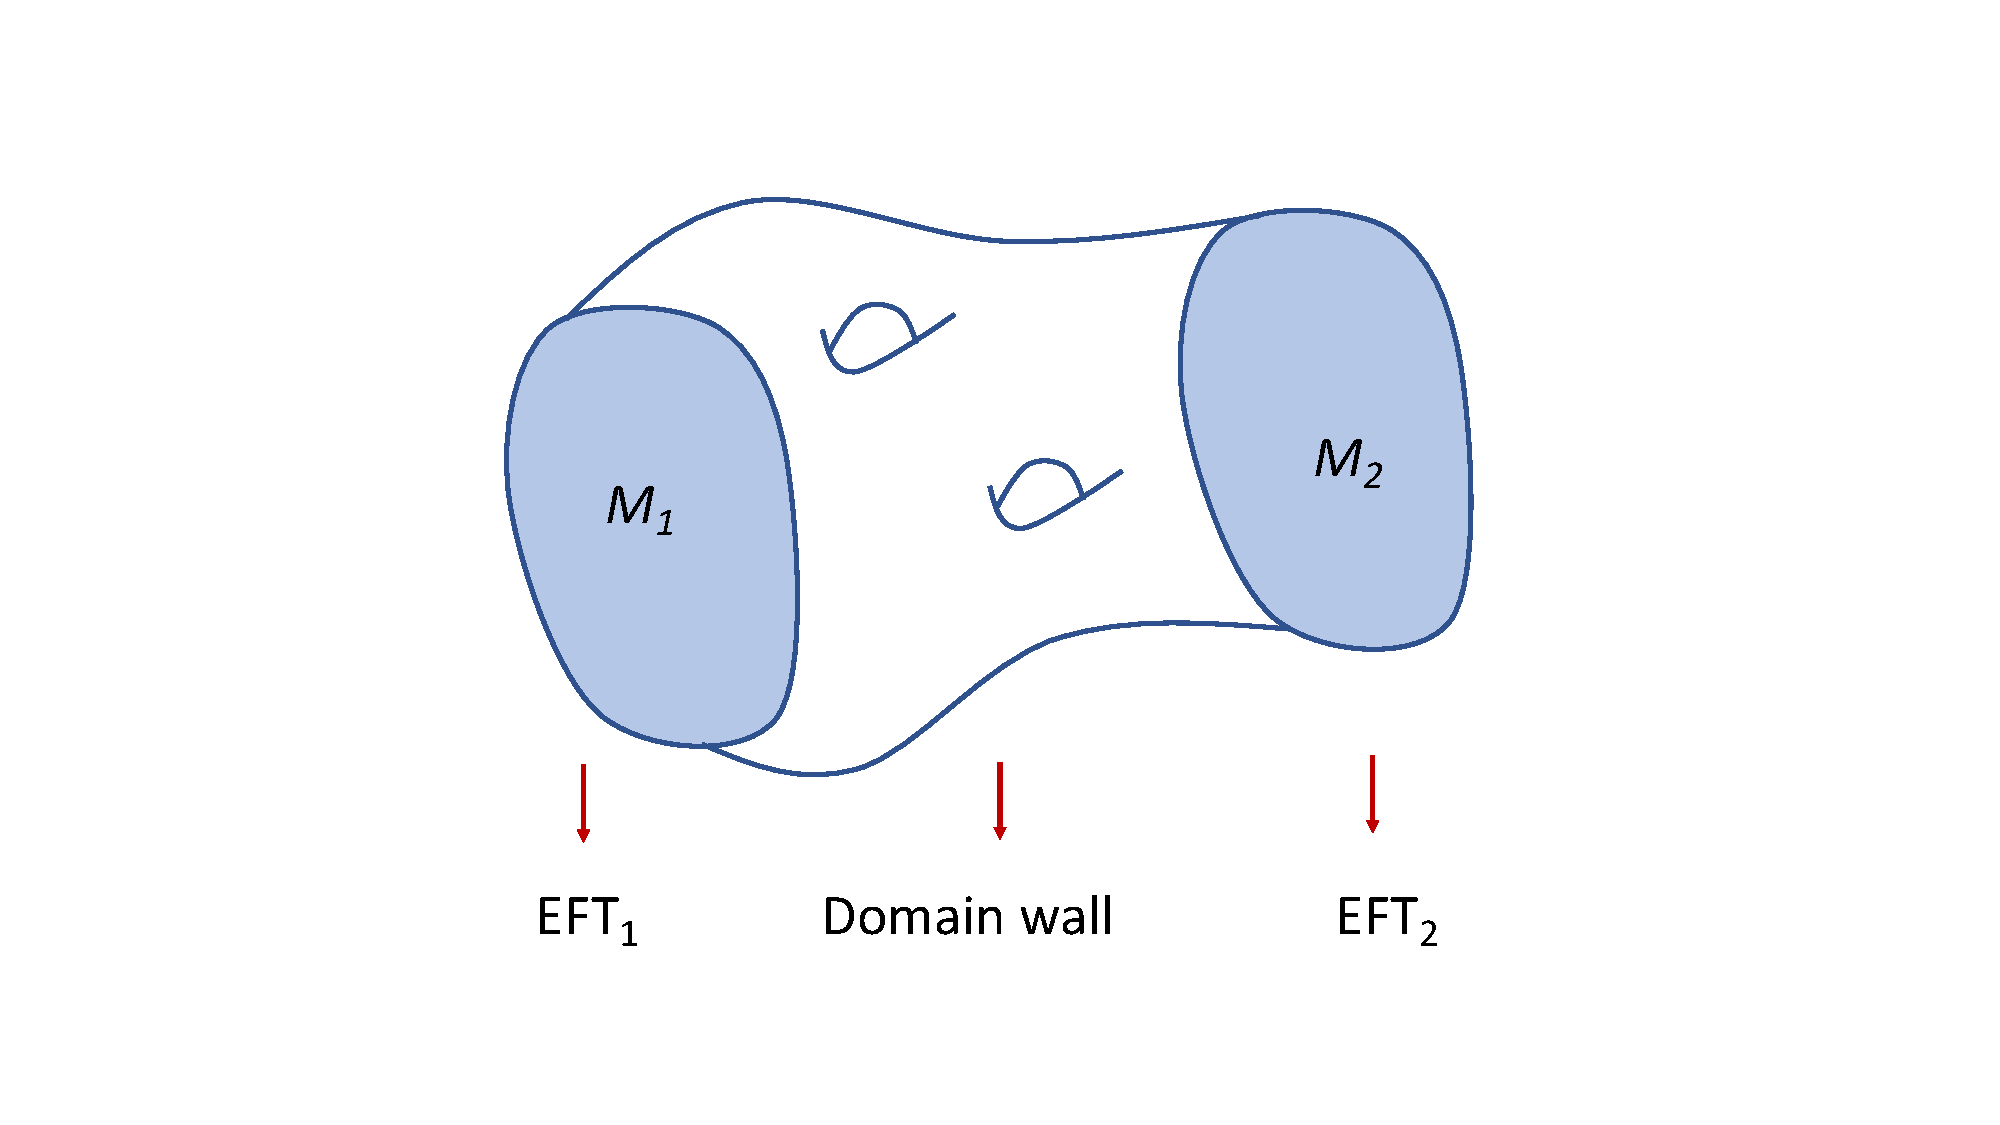
\includegraphics[width=140mm,height=90mm]{Sections/Figures/Cobordism.pdf} 
\vskip -15pt
\caption{A representation of cobordism among two manifolds for which their union is the boundary of another manifold of one extra dimension.} \label{cobordism}
\end{center}
\end{figure}



\item{\it Distance conjecture \cite{Ooguri:2006in}.} 
Consider an effective field theory coupled to gravity with a moduli space, ${\mathcal M}$, parameterised by {\em massless} scalar fields, $\phi_i$, and a metric $\gamma_{ij} (\phi_k)$ which determines the scalar's kinetic terms. 
In standard effective field theories, the consistency and trustworthiness of the dynamics of a scalar field potential $V(\phi)$ is determined by requiring that it does not excite modes with masses above the cutoff, $m \gtrsim \Lambda$.
 As long as this is satisfied, the range of possible values for $\phi$ is not bound by $\Lambda$. The swampland distance conjecture states that this no longer holds if the EFT is consistently uplifted to the UV. 

The swampland distance conjecture states that,  as some modulus approaches a point at infinite {\em geodesic distance} in moduli space, there is an infinite tower of states, which become exponentially massless with the geodesic distance $\Delta\phi$: $m\sim e^{-\Delta\phi}$. These states cannot be neglected from the EFT in this limit. The prime example of such behaviour is when $\phi$ represents the size of an extra dimension and the corresponding tower of states are either the Kaluza-Klein or the winding modes.

As well as infinite limits, the revised distance conjecture also states that for finite displacements, starting from a value $\phi_0$, at a point $\phi_0+\Delta \phi$ infinite towers of modes with mass of order $e^{-\Delta\phi}$ become lighter and lighter with the distance in field space $\Delta\phi$ and so can no longer be neglected from the EFT. Although the conjecture applies to massless scalar fields moving along geodesic trajectories, it could in principle have implications for the field range in single field inflationary models and/or the amount of non-geodesicity in multifield models. However, further work in this direction is needed to establish these possible constraints (see e.g. \cite{Kinney:2018nny, Kinney:2018kew, Palti:2019pca,vanBeest:2021lhn,Grana:2021zvf}).\footnote{ For example, in  \cite{Buratti:2018xjt} it has been shown  that  backgrounds with spacetime varying scalars can  lead to trans-Planckian motion without encountering exponentially falling towers of states. }
 

\begin{figure}[t]
\begin{center}
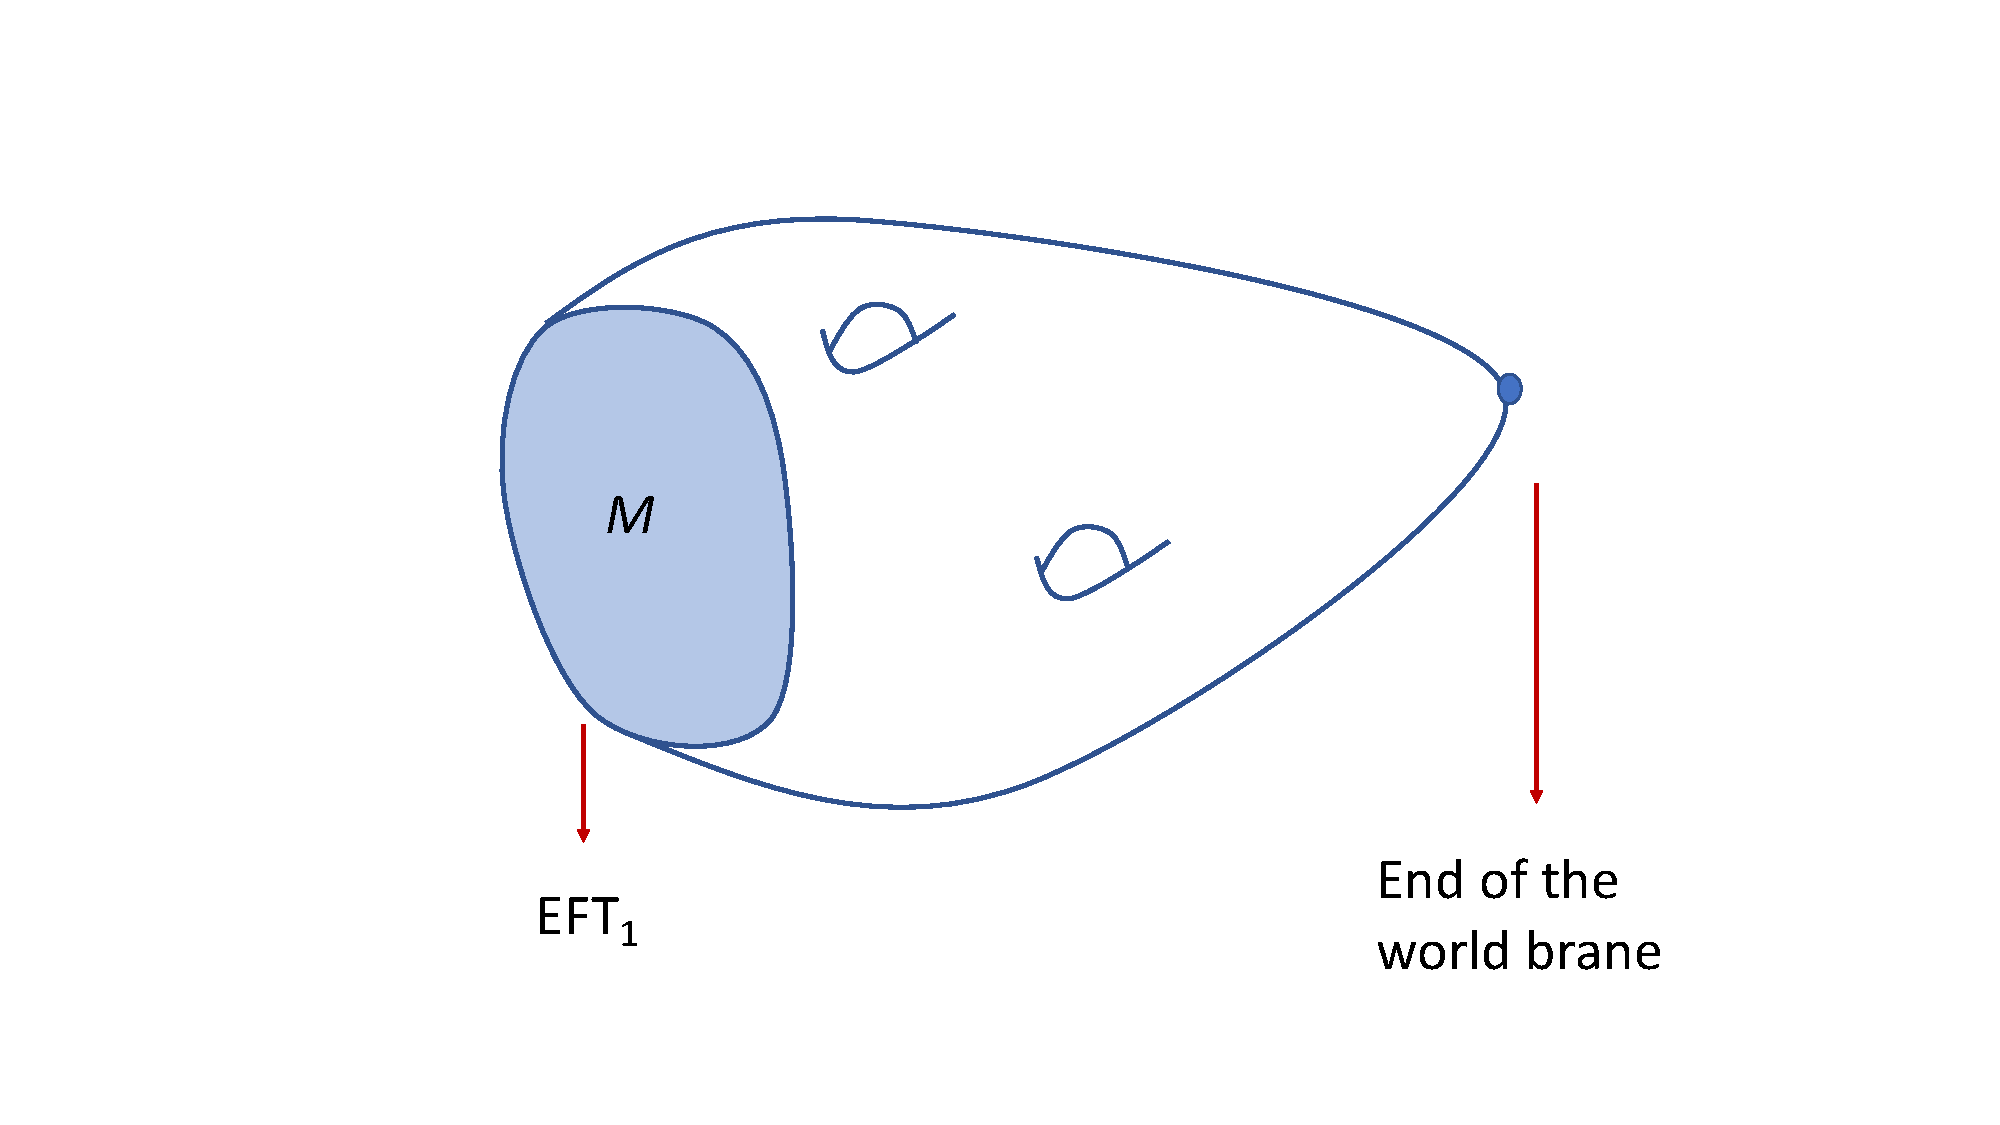
\includegraphics[width=140mm,height=90mm]{Sections/Figures/Cobordism2.pdf} 
\vskip -15pt
\caption{Trivial cobordism with only one manifold in the boundary. The cobordism conjecture states that in this case there should be an end-of-the world configuration.} \label{cobordism2}
\end{center}
\end{figure}


\item{\it Conjectures on  AdS vacua (non-supersymmetric $\&$ supersymmetric):}  Swampland conjectures for non-supersymmetric AdS constructions were proposed in
\cite{Ooguri:2016pdq}. These conjectures are at two levels. The first is motivated by an extension of the weak gravity conjecture; the extension requires that
the equality between electric and gravitational forces is saturated  if and only if the underlying theory is supersymmetric and the states
 under consideration are BPS with respect to the supersymmetry. A consequence of this is that non-supersymmetric AdS solutions supported
 by flux\footnote{A d dimensional AdS solution is said to be supported by flux if a d-form flux field strength   space-fills the AdS space.}  are unstable as they can decay by a brane nucleation process which leads to flux depletion (in a process similar
 to that of \cite{Maldacena:1998uz}). The stronger form of the conjecture removes the requirement that the AdS solution is supported by
 flux and states that  there are no non-supersymmetric AdS solutions in a consistent quantum theory with low energy description in terms of Einstein gravity coupled to a finite number of matter fields. If correct, there will be important  implication not only for moduli stabilisation
 (the AdS vacuum in the LVS scenario is non-supersymmetric) but also for applications of the AdS/CFT correspondence to condensed matter physics, quantum information and hadron physics since the holographic models used in this context have no supersymmetry.  At present, the stronger form of the conjecture does not have much support (see \cite{Baykara:2022cwj} for good evidence in favour of non-supersymmetric AdS vacua in $O(16) \times O(16)$
 heterotic strings). The conjecture can be reformulated in the language of conformal field theories. Conformal field theories dual to Einstein gravity with a finite number of matter fields must satisfy the following (energy) gap condition: they  can have  only a small number of primary fields whose operator products generate all primary fields up to a  energy scale that can be  made parametrically large in the large N limit. The conjecture implies that this condition cannot be met in non-supersymmetric conformal field theories. For attempts to construct such non-supersymmetric conformal field theories meeting this condition see e.g. \cite{Giombi:2017mxl, Gurucharan:2014cva}. 
 
For the relationship of these conjectures of other swampland conjectures, see e.g. \cite{Bernardo:2021vfw}. More recently, it has be put forward that  some  supersymmetric AdS  vacua such as the KKLT AdS solution and pure supergravity AdS lie in the swampland \cite{Lust:2022lfc, Montero:2022ghl}.




\item{\it de Sitter conjecture \cite{Obied:2018sgi}.} It is well known that in string theory both AdS and Minkowski spaces are naturally obtained (mostly because they preserve supersymmetry), while de Sitter space is far more difficult to obtain: a fact which is very important for describing the current acceleration of the Universe through the $\Lambda CDM$ model in terms of the string landscape and early universe inflation. 

The concrete scenarios, such as KKLT and LVS presented in previous sections, provide realisations of de Sitter space from string theory. However, their validity relies on the EFT analysis of perturbative and non-perturbative corrections. As we discussed, the Dine-Seiberg problem that implies the runaway behaviour of the scalar potential for both the volume of the extra dimensions and the dilaton, suggests that in the regime where both perturbative expansions, $g_s$ and $\alpha'$, are under {\it full control}, we should be in the asymptotic runaway region, and so de Sitter vacua at any finite value of the volume or at any non-zero string coupling are in a regime where the approximations cannot be fully trustable. This has led to a bold conjecture stating that there are not actually any de Sitter vacua in a consistent theory of gravity and that the de Sitter vacua found in the literature are only artifacts of the fact that the approximations used are not under full control.\footnote{See also \cite{Cribiori:2020use} for an argument against trustable 4-dimensional dS solutions in $\mathcal{N}=2$ supergravity based on the magnetic weak gravity conjecture.} The original claim was:
\be
\setlength\fboxsep{0.25cm}
\setlength\fboxrule{0.4pt}
\boxed{
|\nabla V|\geq c \frac{V}{\Mp}\,,\qquad 0\leq c \sim {\mathcal{O}}(1)
}
\ee
This condition is clearly satisfied in the Dine-Seiberg runaway regime in which the approximations are under full control. However, the conjecture does not add further information in the weak coupling regions where vacua like KKLT and LVS are claimed to lie. Furthermore, the original conjecture was clearly violated by the Higgs potential (since at the maximum $|\nabla V|=0, V\geq 0$) \cite{Cicoli:2018kdo,Denef:2018etk} (see also \cite{Murayama:2018lie,Choi:2018rze,Hamaguchi:2018vtv}) and a refined version was proposed adding an extra condition on the Hessian of $V$ \cite{Garg:2018reu,Ooguri:2018wrx, Murayama:2018lie}. This conjecture is clearly speculative and less motivated than other swampland conjectures; however, it has motivated further work exploring in more detail  the validity and existence of de Sitter vacua in string theory, which is welcome given the importance of the claim and the challenge.

\item{\it Trans-Planckian censorship conjecture \cite{Bedroya:2019snp,Bedroya:2019tba}.}  It is well known that in inflationary models, microscopic modes redshift due to the expansion of the universe and may become macroscopic and observable at present. If these modes are below the Planck length, it seems to indicate a transfer of modes from the UV to the IR with the UV modes in a regime beyond the validity of the corresponding EFT. The Trans-Planckian censorship conjecture states that in a consistent theory of gravity this UV to IR transfer should not happen, though it does not explain why this should be the case. This puts, for instance, an upper bound on the number of e-folds of inflation. Even though this conjecture has interesting implications for early universe cosmology, the relevance of the constraints on the (time-dependent)  EFT has been questioned in e.g.~\cite{Kaloper:2018zgi,Dvali:2020cgt,Burgess:2020nec,Komissarov:2022gax, Lacombe:2023qfx}.


\end{enumerate}
In summary, the swampland approach brings an interesting perspective to be considered in general discussions of string cosmology. Confirming, discarding or refining these conjectures may lead to relevant progress in the field of string cosmology and, more generally, in principle, to progress in any cosmological implications of consistent theories of quantum gravity. For this much work will be needed.

\subsection{Bubbles of Nothing and the Wave Function of the Universe}

One of the deepest questions a theory of gravity should eventually address is why there is something rather than nothing. This appears a rather philosophical question, as how to define nothingness in a physical theory is unclear. Clearly it is not simply the vacuum state, as we know in 
quantum mechanics the vacuum is not empty. But over the years cosmologists have proposed concrete definitions of nothing (for example, the absence of space, time and matter). The first explicit example was Witten's bubble of nothing (BON) \cite{Witten:1981gj} illustrated in figure \ref{bon}. When considering simple compactifications of five-dimensional Kaluza-Klein theories, he found a transition from the flat five dimensional metric corresponding to a circular fifth dimension of radius $R$: $ds_5^2= ds_4^2+R^2 d\phi^2$, mediated by an instanton with Euclidean metric:
\be
ds^2=\frac{dr^2}{1-R^2/r^2}+r^2\left(d\theta^2+\cos^2\theta d\Omega_2^2 \right)+ \left(1-R^2/r^2\right) R^2 d\phi^2.
\ee
Similar to the Euclidean Schwarzschild metric, this is non-singular even at $r=R$. But this is a minimum value of the coordinate $r$. For large $r$ the metric is asymptotically flat. So this instanton mediates a transition from a flat spacetime with a circle of radius $R$ to a spacetime with maximum value of $r$ where the fifth dimension collapses which we may identify as a {\it bubble of nothing}. The interesting point is that after nucleation the further evolution of the bubble is through expansion at the speed of light, as can be seen by the Wick rotation $\theta\to it$. Since
$\cos\theta \to \cosh t$ the bubble radius increases exponentially with time eating up the full spacetime. In the 5d case, 
this transition depended on the non-existence of supersymmetry and was considered without taking into account moduli stabilisation of the extra dimension. Generalisations to 6d with moduli fixed by fluxes have been found with the similar dramatic outcome \cite{Blanco-Pillado:2010xww,Brown:2011gt}. Furthermore, it was recently argued that these bubbles of nothing are ubiquitous in string compactifications \cite{GarciaEtxebarria:2020xsr} and may represent eventual sources of instabilities (although being non-perturbative, the decay rate may be much suppressed).
\begin{figure}[t]
\begin{center}
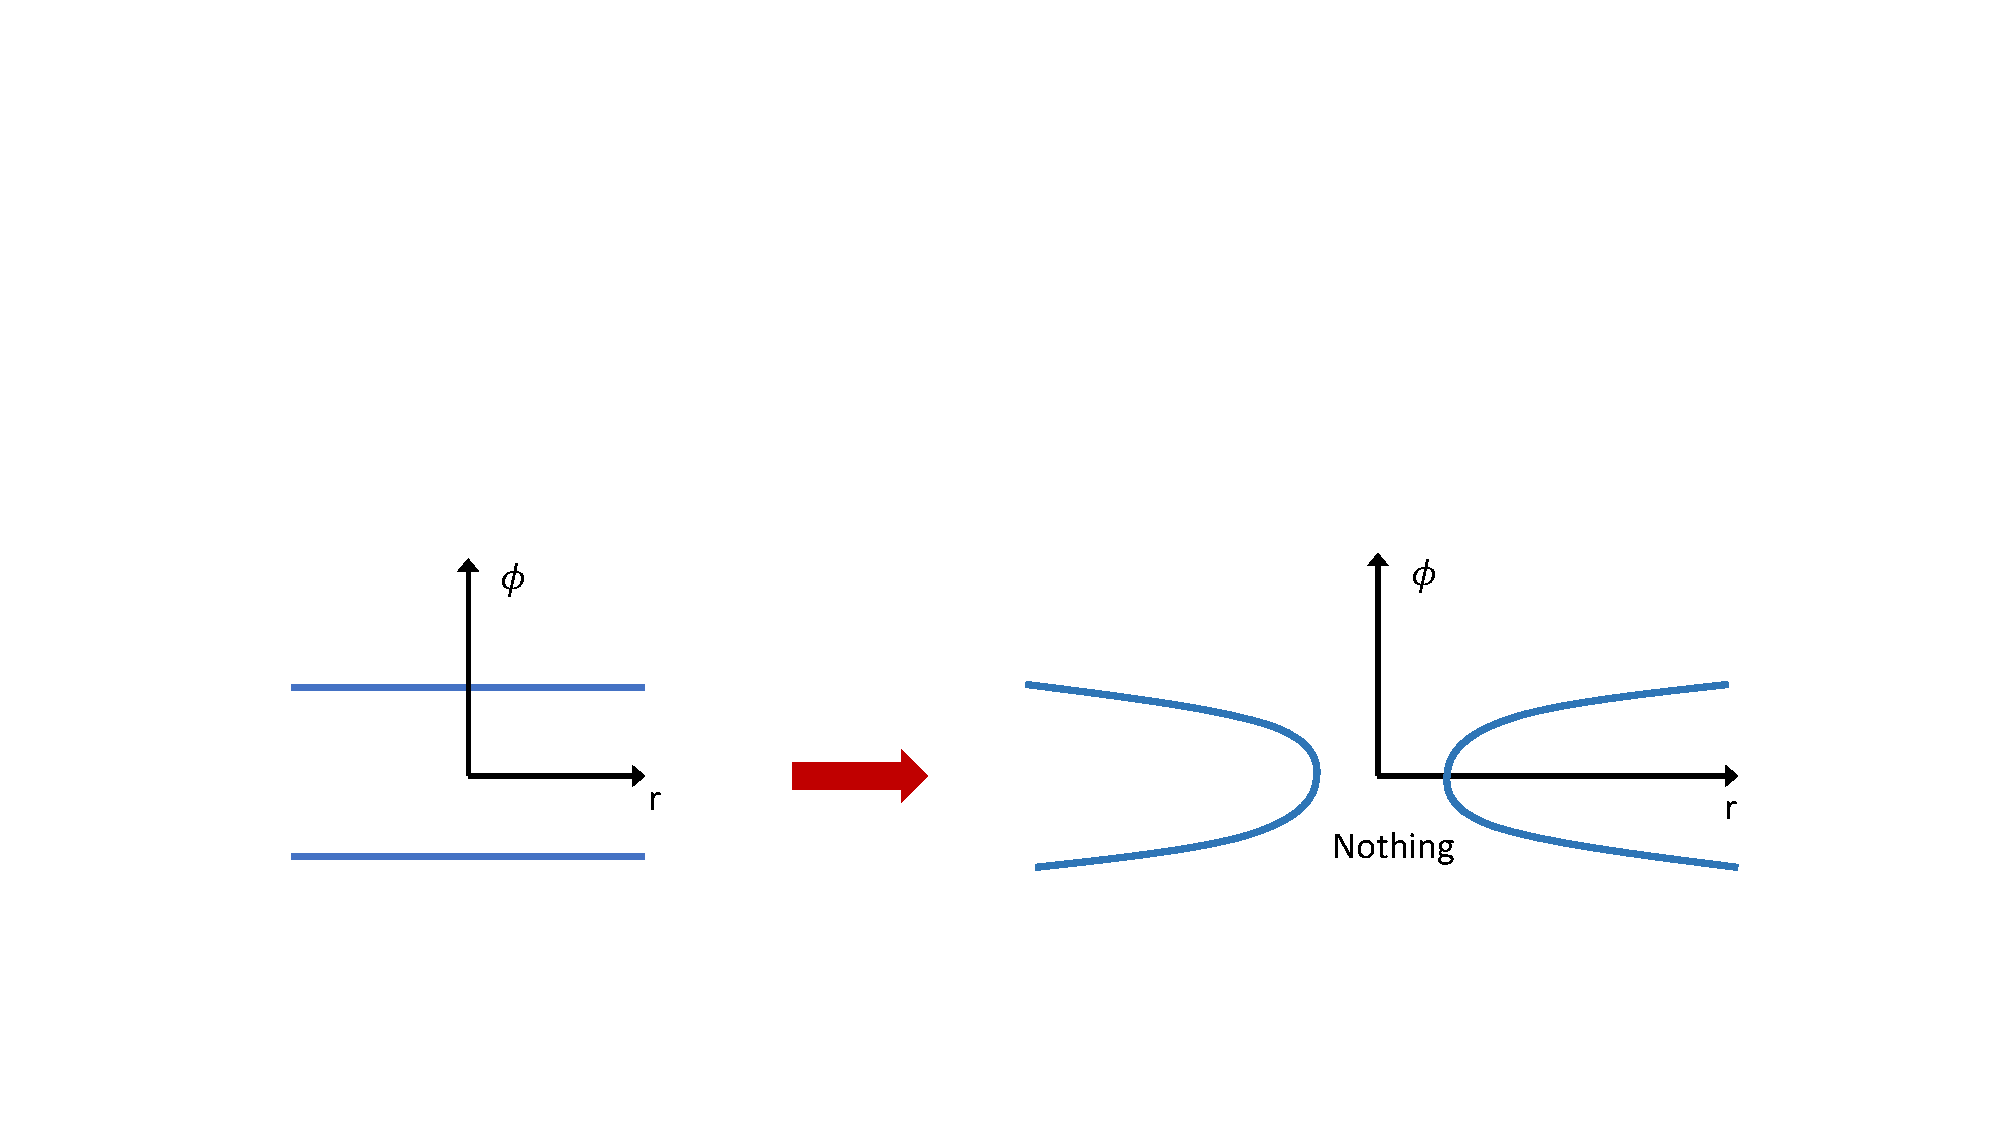
\includegraphics[width=170mm,height=50mm]{Sections/Figures/BON.pdf} 
\caption{An illustration of the Bubble of Nothing scenario: a transition resulting to an expanding absence of space-time. On the left we have the flat 4d in the horizontal  and the extra dimension in the vertical with the two horizontal lines identified in a circle compactification. On the right the transition to the bubble of nothing. For large $r$ it is as in the left but for smaller values of $r$ at some point the extra dimension collapses and a bubble of nothing appears (a cross section is shown) and expands in time.} \label{bon}
\end{center}
\end{figure}

The second appearance of nothing was in the {\it creation out of nothing} scenario of Vilenkin \cite{Vilenkin:1982de,Vilenkin:1983xq,Vilenkin:1984wp} and the subsequent {\it wave function of the universe} of Hartle and Hawking \cite{Hartle:1983ai}. See also\cite{Linde:1983mx,Rubakov:1999qk,Hartle:2022jkt}. This  defines, within the domain of semiclassical gravity, a concrete proposal to describe the beginning of the universe from a state with no spacetime. So, in a sense it is the opposite of the bubble of nothing picture. 

From simple mini-superspace arguments the transition from nothing to a de Sitter space with cosmological constant given by $H^2>0$ is found to be of order 
\be
{\mathcal P}=|\Psi|^2\propto\, e^\frac{\eta\, \pi}{2G_4H^2},
\ee
with $\eta=+1$ for Hartle-Hawking boundary conditions (the no boundary proposal in which the nucleated universe is a superposition of expanding and contracting ones) and $\eta=-1$ for the Vilenkin or tunneling transition (for which the boundary conditions are such that they only give an expanding universe). Note that, up to normalisation factors, the Hartle-Hawking wave function favours smaller values of the cosmological constant, making it hard to justify inflation, whereas the Vilenkin normalisation prefers larger values of $H^2$. All these discussions are only within a simplified picture of mini-superspace and semiclassical gravity and, in principle, need to be further studied, especially once a proper quantum gravity theory is at hand. This has been a challenge for string theory and, despite several attempts, the study of such transitions is still in its infancy.

Note that this approach is similar in spirit to the vacuum transitions initiated by Coleman and de Luccia (CDL) which have been inherited in the discussions of the landscape. However, contrary to CDL transitions, here there is no bubble nucleated but instead a full spacetime. This can be done for de Sitter since it has finite volume but for AdS and Minkowski it may require introducing a cut-off in order to quantify the corresponding probability. Furthermore, contrary to the CDL case in which naturally the transition gives rise to an open universe, here, the de Sitter slicing that gives finite volume corresponds to a closed universe \cite{Hartle:2013oda,Cespedes:2020xpn}. This is important since there have been claims that the main general prediction of the string landscape is that it predicts open universes \cite{Freivogel:2005vv,Kleban:2012ph} and if eventually, in the maybe long future, open universes would be ruled out it could  be a strong argument against the landscape. But if closed universes can be created from nothing, settling the curvature of the universe may only differentiate between the two mechanisms. Clearly further studies in these directions are needed.\footnote{An important direction is
bubble stability, see e.g \cite{Johnson:2019tgc} for a recent analysis.} For string theoretical discussions of the wave function of the universe see for instance \cite{Ooguri:2005vr,Brustein:2005yn}.

\subsection{Holography and Cosmology}

The main theoretical development in string theory over the past 25 years has been holography. A gravitational theory in $d$ dimensions is equivalent to a non-gravitational theory in $(d-1)$-dimensions. One old motivation for this equivalence is the well known fact that the black hole entropy, being an extensive quantity, is proportional to the area of its horizon rather than to the internal volume of the black hole. 
The AdS/CFT correspondence now represents the best concrete definition of quantum gravity in anti-de Sitter space (AdS) since, at least in principle, the non-gravitational conformal field theory (CFT) on the boundary of AdS is understood, and any quantum aspects of the gravitational theory can be referred to concrete questions on the CFT side.

Although technically AdS/CFT remains a conjecture,
the evidence for the correspondence is by now overwhelming. In particular, this correspondence has provided a framework which 
allows the black hole loss of information puzzle stated by Hawking almost 50 years ago to be addressed. Holography 
 indicates that, as the CFT side is a standard quantum system, information cannot be lost. Therefore, if the equivalence is correct, 
information also cannot be lost within the gravitational system. Furthermore, using holographic arguments it has also recently been possible to calculate explicitly the entanglement entropy of black holes showing the Page curve behaviour that would be 
expected if the information is not lost\footnote{For studies of implication of entanglement (in particular Bell inequalities) in the cosmological context see \cite{Maldacena:2015bha, Choudhury:2016cso}.}.

It is therefore very appealing to try to extract cosmological implications of holography. Even though our universe is not of the AdS type, several approaches have been proposed, aiming to extend the success of AdS/CFT to cosmological questions. The general topic of holography is so vast 
that we will touch on it even more briefly than for previous subjects and refer the reader to the literature for more details. For recent reviews see for instance \cite{Anninos:2012qw, Flauger:2022hie}.

\begin{enumerate}
\item {\it AdS/CFT  and density perturbations in inflation.} 

One possibility to use AdS/CFT for inflation is to consider a simple potential with two minima with opposite signs of the cosmological constant. 
One minimum corresponds to a stable AdS vacuum and the other to a nearby metastable dS vacuum. The bulk geometry 
near the AdS vacuum is described by boundary CFT and so this can be used to extract information about bubbles of the dS phase from the CFT spectrum \cite{Freivogel:2005qh} (see however \cite{DeAlwis:2019rxg}) and, through analytic continuation, connect the correlators from AdS/CFT to a potential dS/CFT .

In a different direction, assuming that inflationary cosmology has a CFT dual there have been explicit efforts to quantify this 
relation by computing density perturbations using a QFT dual. In particular, known inflationary results regarding
 density perturbations are reproduced in the weak gravity regime. Exploring the domain of strongly coupled gravity by working with 
 the weakly coupled QFT offers an alternative phenomenology to inflation in which an almost scale invariant spectrum of 
 perturbations is also obtained. See e.g. \cite{Freivogel:2005qh, McFadden:2009fg, Bzowski:2012ih, Kundu:2014gxa} for concrete calculations in this
  interesting direction.

\item {\it dS/CFT and dS/dS proposals.} 

A dS/CFT correspondence
 was proposed in \cite{Strominger:2001pn}, following parallels with the
well established AdS/CFT correspondence,
 motivated by the close connection between dS and AdS spaces.
The argument is that a boundary at infinity of, say,  dS$_4$ corresponds to a Euclidean $R_3$
space for which the symmetry group of de Sitter space, $SO(4,1)$ acts as the conformal group
of the Euclidean $R_3$, suggesting that a conformal field theory on this boundary is dual to the full 4D gravity theory in de Sitter space.

 One of the interesting outcomes of
 this conjecture is that the renormalisation group parameter can be identified with
time, in much the same way it was identified with the extra spatial 
coordinate in the AdS/CFT case \cite{Strominger:2001gp}. One simple way to see this possibility is 
by writing the dS$_4$ metric in FRW coordinates ($k=0$) as
\be
ds^2\ = \ -dt^2\ + \ e^{Ht}\ d\vec{x}^{\,\,2},
\ee
with $\vec{x}$ the spatial coordinates 
 and $H$ the Hubble parameter. 
 
 The interesting observation is that this
 metric is invariant under
$t\rightarrow t+\lambda$, $\vec{x}\rightarrow e^{-\lambda H}\vec{x}$ which 
generates time evolution in the 4D bulk and scale transformations on the
 Euclidean boundary.
Late times (large values of $\lambda$) correspond to small distances (UV
 regime) whereas earlier 
times correspond to low energies and the IR regime.
Generic expressions for the scale factor $a(t)$ will not have this symmetry,
but if we assume that
$H(t)$ goes to a constant both in the infinite past and infinite future we can 
follow the time evolution
between two fixed points under the renormalisation group, which could
 eventually be identified
with early universe inflation and also current acceleration. 

The monotonic evolution in time fits well  with the 
expected c-theorem of field theories, holding in 2D, and the extension to the a-theorem in 4d.
The RG flow then corresponds to the direction from future to past. 

As a side note, the S-branes mentioned previously were
 an attempt to bring this correspondence closer to the AdS/CFT one, with the
 S-branes playing the role of the D-branes in the
boundary (the Euclidean $R_3$ in the example above).

A final independent and interesting alternative is the dS/dS correspondence in which a dS space is proposed to be dual to another dS space in one dimension less \cite{Alishahiha:2004md,Dong:2010pm}. This is partly based on the simple observation that the de Sitter dS$_d$ metric in $d$ dimensions can be seen as a warped compactification to dS$_{d-1}$:
\be
ds_d^2=d\omega^2+\sin^2\left(\frac{\omega}{R_{dS}}\right) ds_{d-1}^2.
\ee
Similarly to AdS/CFT, this implies an emergent spatial dimension and warped throats (two in this case since the warp factor vanishes at $\omega=0,\pi R_{dS}$), but contrary to AdS/CFT the dual is no longer a field theory without gravity but now a lower dimensional de Sitter space with a massless graviton.

Even though de Sitter space realisations in string theory are of interest, these potential dS/CFT or dS/dS dualities are not yet under firm grounds, unlike the AdS/CFT case, and much work needs to be done to turn these proposals into something useful for cosmology.

Further proposals for holography and cosmology have been put forward. See for instance \cite{Banks:2003ta}.

\item {\it Islands and cosmology}

A more recent development relates to the progress regarding the information loss paradox in black holes. The main new ingredient here is the concept of quantum extremal surfaces (QES) \cite{Ryu:2006bv,Hubeny:2007xt,Faulkner:2013ana,Engelhardt:2014gca} to generalise the expression for the von Neumann entropy. This prescription gives rise to a time evolution of the entropy such that it increases monotonically up to a maximum point where it starts decreasing, giving rise to what is called a Page curve as required for a unitary evolution  to address the information loss paradox. The key component of this calculation is an entanglement  {\it island} which is a region behind the black hole horizon that hosts the corresponding  degrees of freedom that avoid information loss \cite{Penington:2019npb,Almheiri:2019psf}.

The details of these results are beyond the scope of this review (for a review with all the relevant references see for instance \cite{Almheiri:2020cfm}). However, a notable point is that these results were achieved without the need for a full UV completion of semiclassical gravity. This gives more credibility to semiclassical approaches to quantum cosmology, such as the wave function of the Universe and vacuum transitions discussed above. Furthermore, concepts like quantum extremal surfaces and islands may also play an important role for cosmology. This has been recently explored in 
%
\cite{VanRaamsdonk:2020tlr,Hartman:2020khs,Chen:2020tes,VanRaamsdonk:2021qgv,Geng:2021wcq,Pasquarella:2022ibb, Bousso:2022gth} but it is fair to say that this direction is still in an infancy and there is much to be explored. 

\item{\it Emergence of spacetime}

One point that may be worth pointing out is the recent ideas regarding the emergence of time.  From the original AdS/CFT correspondence, it is clear that not only gravity but also at least one spatial dimension is emergent from the boundary CFT theory (in one less dimension and no gravity). More recent studies of the closed connection between gravitational theories and quantum entanglement have led to the proposals of getting spacetime from entanglement. The proposal of ER=EPR (Einstein-Rosen wormhole equivalent to the Einstein-Podolsky-Rosen entanglement) is a variation of this. Contrary to the emergence of spatial dimensions, the emergence of time has been more challenging to implement. But recent work has been done in this direction. See for instance \cite{Leutheusser:2021frk, Witten:2021unn, Chandrasekaran:2022eqq, Chandrasekaran:2022cip, Leutheusser:2022bgi,Cotler:2023xku}. These subjects fall beyond the scope of the present review and we refer the reader to the papers mentioned and references therein.





\end{enumerate}

Other approaches to string cosmology have been proposed with different levels of development. We would like to note the cosmology of matrix models, which, even though it has not been much explored, matrix models \cite{Banks:1996vh,Ishibashi:1996xs} are one of the few proposals (together with AdS/CFT)  for a non-perturbative formulation of string theory and may deserve further study. We refer to the recent review \cite{Brahma:2022ikl} for the progress and challenges of this approach. 

\enddocument

 \newpage





\input{Sections/OutlookV2}


\appendix



\addcontentsline{toc}{section}{References}
%may need this
%\bibliographystyle{utphys}
\bibliography{refsIZV2}


\end{document}

\endinput



\underbrace{\nu_e + n}_{\rm before} 
\underbrace{6x - 4x}_{2x}



% corchetes con ejemplos:
\begin{displaymath}
y = \left\{ \begin{array}{ll}
a & \textrm{if $d>c$}\\
b+x & \textrm{in the morning}\\
l & \textrm{all day long}
\end{array} \right.
\end{displaymath}


%Colored box:
%colback= background colour 
% manual colorbox:https://osl.ugr.es/CTAN/macros/latex/contrib/tcolorbox/tcolorbox.pdf
\begin{tcolorbox}[colback=white, title=My heading line]
\begin{enumerate}
    \item Cambiar notacion
    \end{enumerate}
\end{tcolorbox}

\overset{\chi}{\longrightarrow}

%SUBEQUATIONS:
\begin{subequations}
 \begin{align}
     S_{\rm EH} &= \frac{1}{2\kappa^2}\,\int\,\d^4 x\,\sqrt{-g}\,R, \\
     S_{\phi} &= -\int\,\d^4 x\,\sqrt{-g}\left[\frac{b}{2} (\partial\phi)^2+ M^4 C^2(\phi)\,\sqrt{1+\frac{D(\phi)}{C(\phi)}\,\left(\partial \phi\right)^2} + V(\phi)\right], \label{eq:Sphi}\\
     S_m &= - \int\,\d^4 x\,\sqrt{-\tilde{g}}\,{\mathcal L}_M (\tilde{g}_{\mu\nu}),
 \end{align}
\end{subequations}

%SPLIT EQUATION
\begin{equation}
\begin{split}
a&= b \\
c &= d \\
&= f \,,
\end{split}
\end{equation}

% BOXED SUBEQS:
\begin{subequations}
\begin{empheq}[box=\widefbox]{align}
 &a \,, \\
&b\,.
\end{empheq}
\end{subequations}

\stackrel{ ... }{=}

\be\label{eq:mcCB}
\setlength\fboxsep{0.25cm}
\setlength\fboxrule{0.4pt}
\boxed{
m_C\sim 2E_A}\,,
\ee

%%
